\documentclass[10pt,a4paper]{article}
\usepackage[utf8]{inputenc}
\usepackage{amsmath}
\usepackage{amsfonts}
\usepackage{amssymb}
\usepackage{graphicx}
\usepackage{epstopdf}
\usepackage{inputenc}
\usepackage[a4paper, total={150mm,250mm}]{geometry}
\usepackage{graphicx}
\usepackage{hyperref}
\usepackage[dvipsnames, table]{xcolor}
\usepackage{subcaption}
\usepackage{fancybox, graphicx}
\usepackage{tikz}
\usepackage{array}
\usepackage{ulem}
\usepackage{enumitem}
\usetikzlibrary{shadows}
\usepackage{listings}
\usepackage{bm}
\usepackage{lmodern,textcomp}
\usepackage{listings}
%\usepackage[english]{babel}


\makeatletter
\renewcommand\@biblabel[1]{\textbullet}
\makeatother
\newcommand{\question}[5]{
{#1}
\begin{enumerate}[label=\textbf{\alph*)}]
	\item {#2}
	\item {#3}
	\item {#4}
	\item {#5}
\end{enumerate}
}


\newcommand{\nline}{\\~\\}
\usepackage{tikz}
\hypersetup{
    colorlinks=true, %set true if you want colored links
	linkcolor=black,
    linktoc=all,     %set to all if you want both sections and subsections linked 
    urlcolor=blue
}
\title{{\Huge\textbf{USDE - Notes}
\\ \LARGE Unstructured Streaming and Data Engineering
\vspace{0.5em}
\\ \large \textbf{Professors}: Emanuele Della Valle - Marco Brambilla  \linebreak
\\ \small \textbf{Author}: Simone Staffa \linebreak

\vspace{5em}
\begin{figure}[h!]
 \hfill 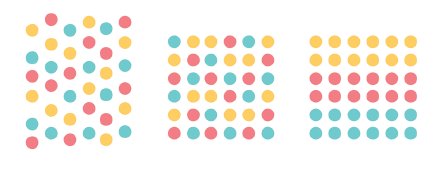
\includegraphics[width=300pt]{images/cover.png}\hspace*{\fill}
  \label{fig:polimi}
\end{figure}
}
\vspace{1em}
\small{
Released with Beerware License, Rev. 42 (https://spdx.org/licenses/Beerware.html) \linebreak
“As long as you retain this notice you can do whatever you want with this stuff. If we meet some day, and you think this stuff is worth it, you can buy me a beer in return”}
}
\begin{document}
\maketitle
\clearpage
\tableofcontents
\clearpage
\section{Introduction (Course motivation)}
\subsection{Data-driven Decision Making for Data-driven Organizations}
In many organizations decisions are made by "questionable" methodologies such as
\begin{itemize}
	\item \textbf{Hi}ghest \textbf{P}aid \textbf{P}erson \textbf{O}pinion (HiPPO): when Galileo tried to say that the earth cycles around the sun, the pope (the HiPPO) stated that heliocentrism was impossible.
	\item \textbf{Flipism}: all decisions are made by flipping a coin (randomly)
\end{itemize}
This could have been the right approach in the '70s... but in the Digital Era one can dream of data-driven organization, taking decisions using data.
\center{\textit{"\textbf{Decisions} no longer have to be made in the dark or based on gut instinct; they can be \textbf{based on evidence, experiments and more accurate forecasts}", McKinsey}}
\\ \vspace{0.5em}\raggedright
Data-driven organizations
\begin{itemize}
	\item \textbf{perform better}: the data shows where they can streamline their processes
	\item \textbf{are operationally more predictable}: data insights fuel current and future decision making
	\item \textbf{are more profitable}: constant improvements and better predictions help to outsmart the competition and improve innovation.
\end{itemize}
\subsection{Solving problems with Big Data, Data Science and ... Data Engineering}
\begin{figure}[h!]
 \hfill 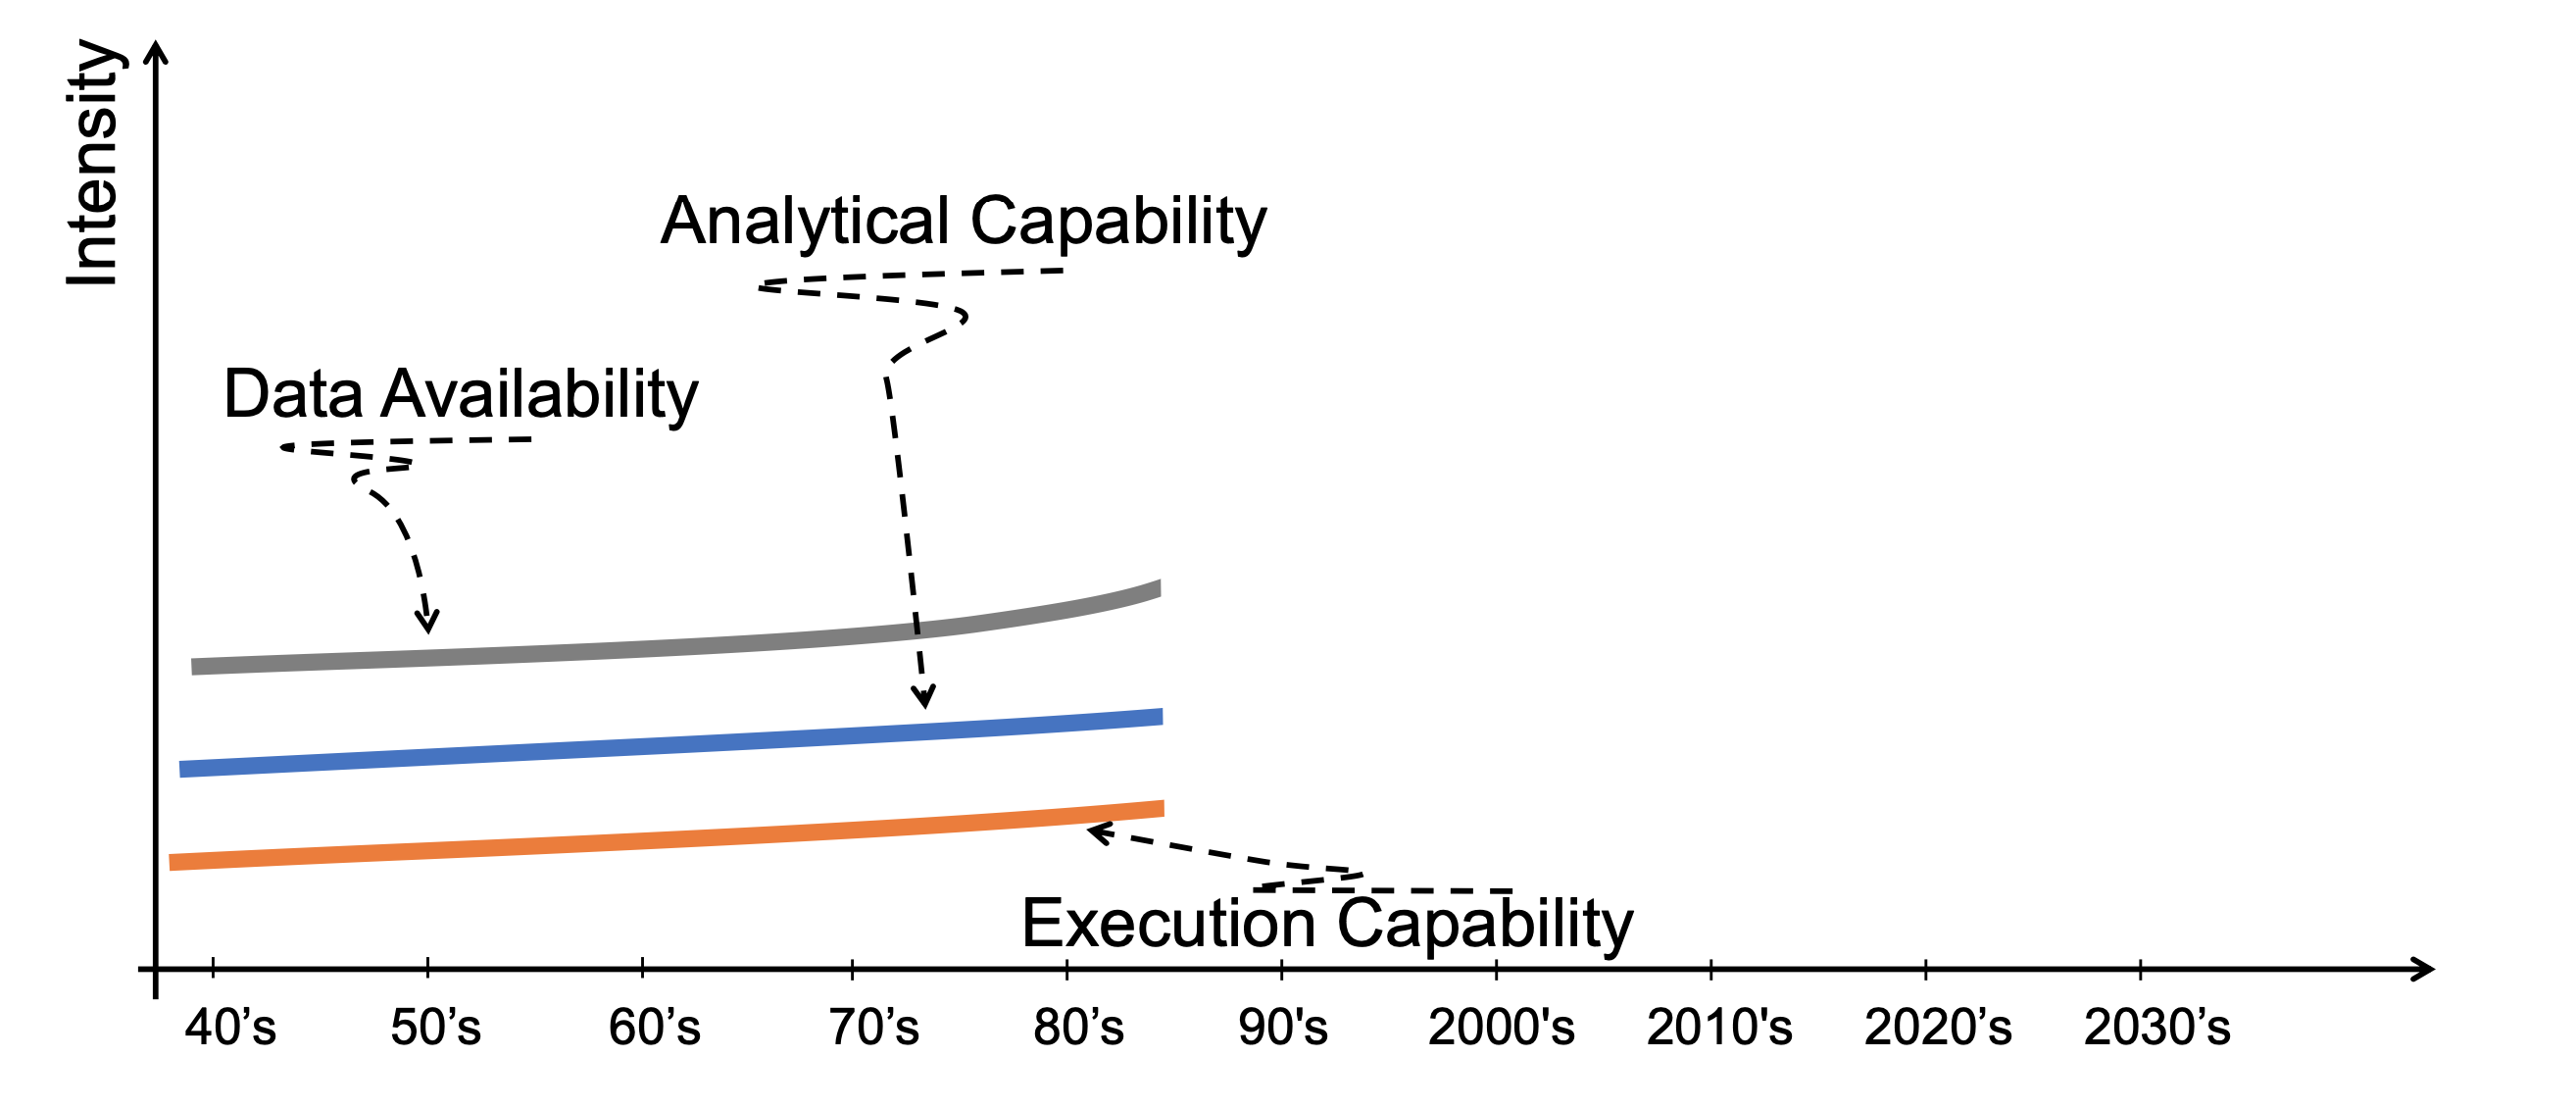
\includegraphics[width=300pt]{images/data-analysis.png}\hspace*{\fill}
  \label{fig:data-analysis}
  \caption{Up until '90s the data available was growing together with our analytical and execution capabilities.}
\end{figure}
\begin{figure}[h!]
 \hfill 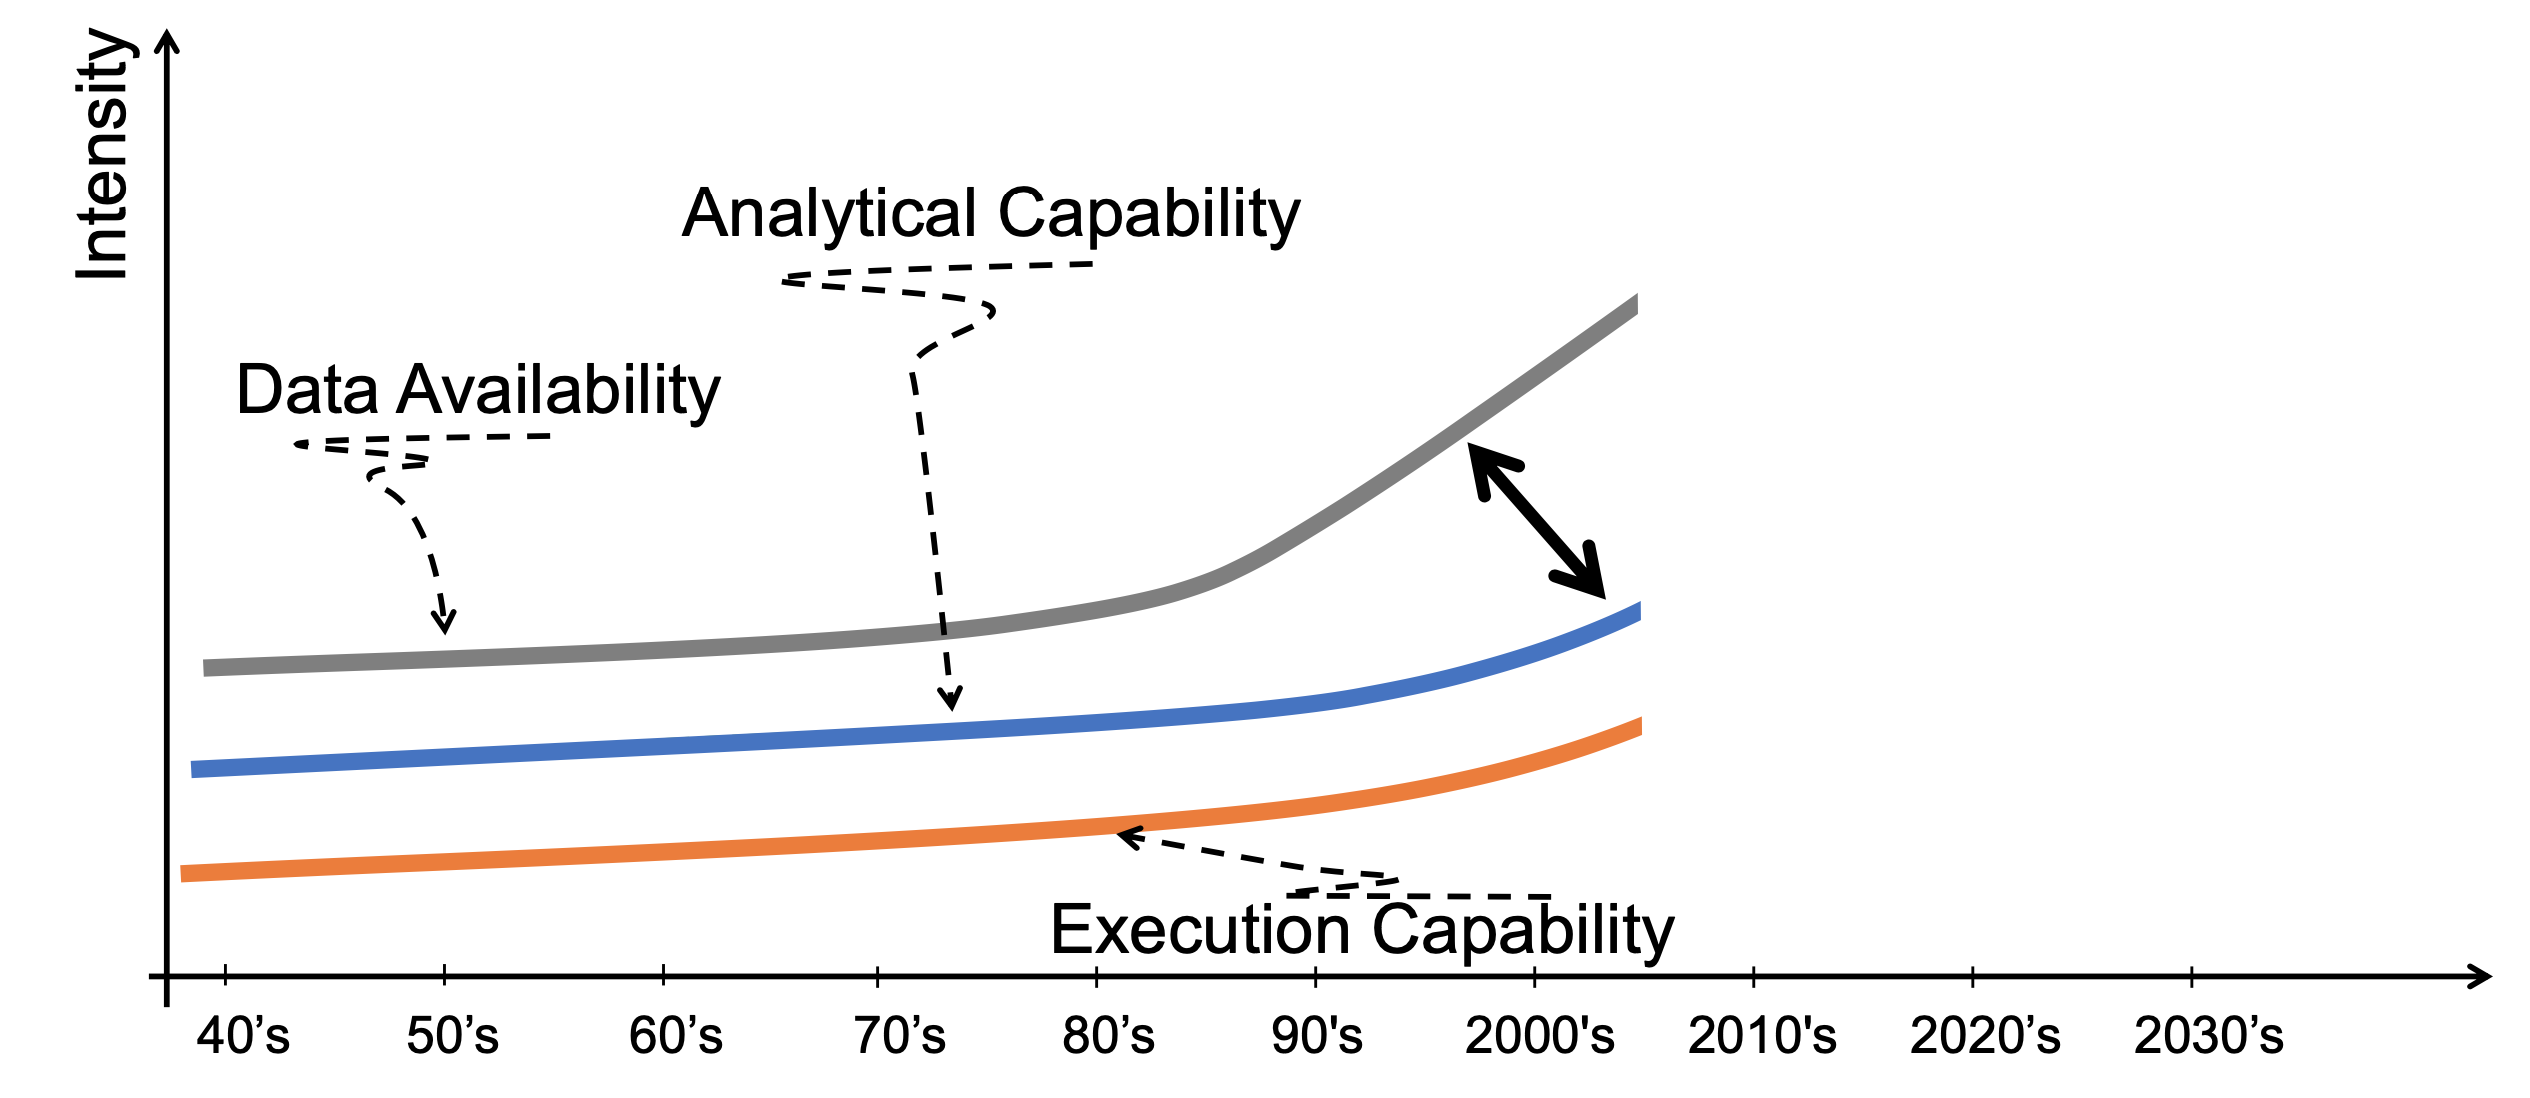
\includegraphics[width=300pt]{images/big-data.png}\hspace*{\fill}
  \label{fig:big-data}
  \caption{With the new millenium we have the appearence of Big Data. Data availability is growing fast and the digital revolution gap is growing.}
\end{figure}
\subsubsection{What's Big Data?}
Big data is a term that describes the large volume of data – both structured and unstructured – that inundates a business on a day-to-day basis. \\
IBM data scientists break big data into four dimensions: 
\begin{itemize}
	\item \textbf{Volume} (data at scale): volume is increasing, we have more and more data. Curiosity: in Italy is rare to find companies work with more than 20 Terabytes of data (only big customers)
	\item \textbf{Variety} (data in many form): structured, unstructured (or semi-structured e.g., graph), text, multimedia
	\item \textbf{Velocity} (data in motion): analysis of streaming data to enable decision within fractions of a second (real time decision and data analysis while data are coming). This is not a property of data but is specifically related to the kind of analysis we want to achieve.
	\item \textbf{Veracity} (data uncertainty): managing the reliability and predictability of inherently imprecise data type. This is not a property of data, it regards the quality of data. For 1 purpose the data are good, for another purpose the same data may not be good (or useful).
\end{itemize}
\begin{figure}[h!]
 \hfill 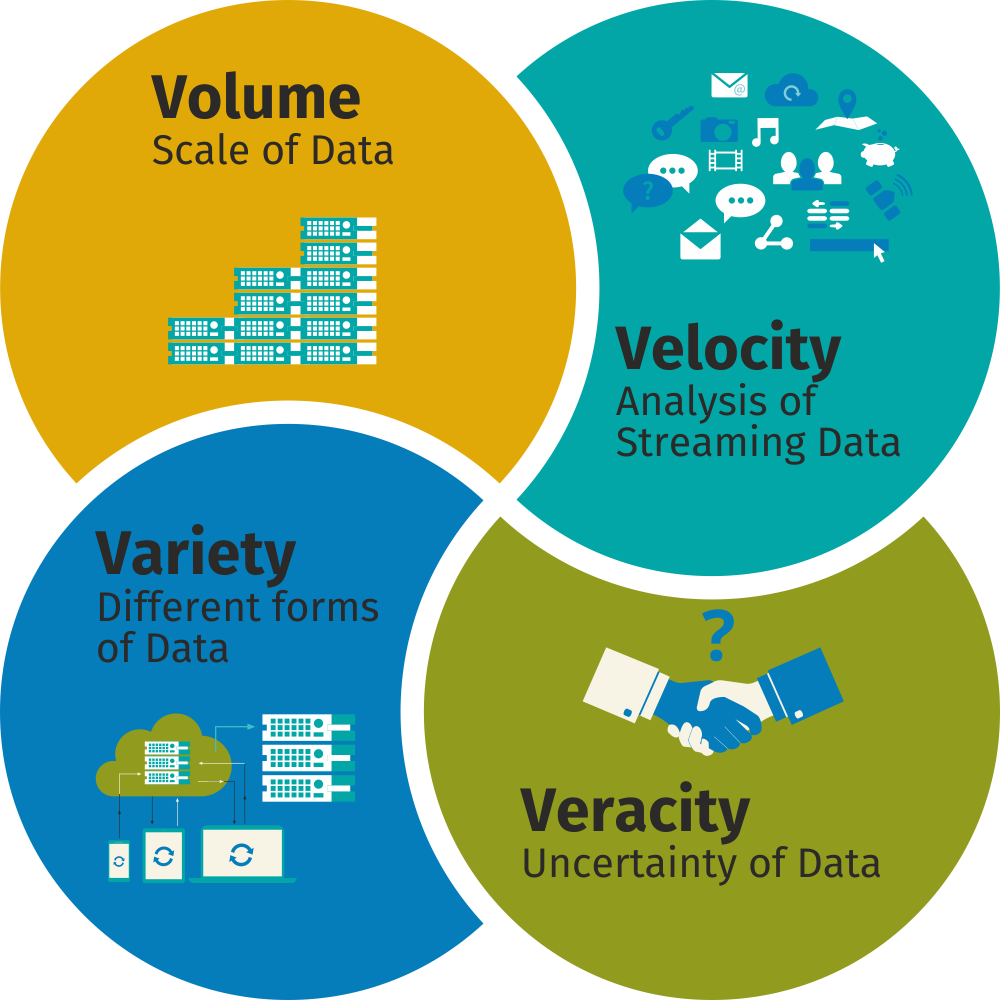
\includegraphics[width=200pt]{images/4v.png}\hspace*{\fill}
  \label{fig:4v}
  \caption{With the new millenium we have the appearence of Big Data. Data availability is growing fast and the digital revolution gap is growing.}
\end{figure}
Big Data techs are like "crude oil" that we have to:
\begin{itemize}
	\item Extract
	\item Transport in mega-tankers
	\item Ship through pipelines
	\item Store in massive silos
\end{itemize}
\begin{figure}[h!]
 \hfill 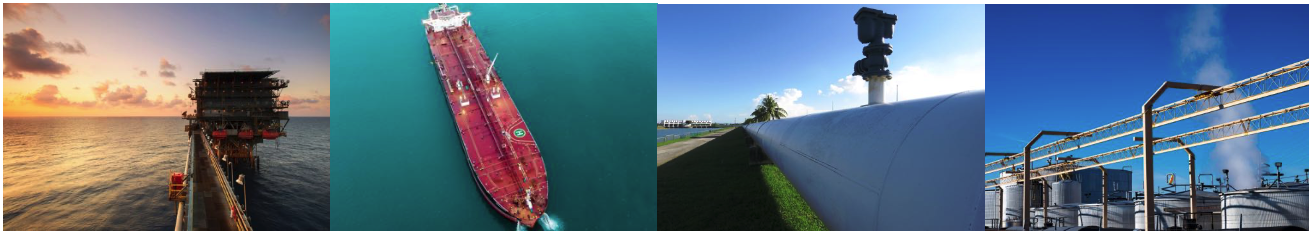
\includegraphics[width=300pt]{images/crude-oil.png}\hspace*{\fill}
  \label{fig:crude-oil}
\end{figure}
\subsubsection{What's Data Science}
The Science (and Art) of:
\begin{itemize}
	\item \textbf{Discovering} what we don’t know from data
	\item Obtaining \textbf{predictive, actionable insight} from data
	\item \textbf{Creating Data Products} that have business impact now
	\item \textbf{Communicating} relevant business stories from data
	\item \textbf{Building confidence} in decisions that drive business value
\end{itemize}
\textbf{Data scientists} are a new breed of analytical data expert who have the technical skills to solve complex problems – and the curiosity to explore what problems need to be solved. They’re part mathematician, part computer scientist and part trend-spotter. And, because they straddle both the business and IT worlds, they’re highly sought-after and well-paid.
\begin{figure}[h!]
 \hfill 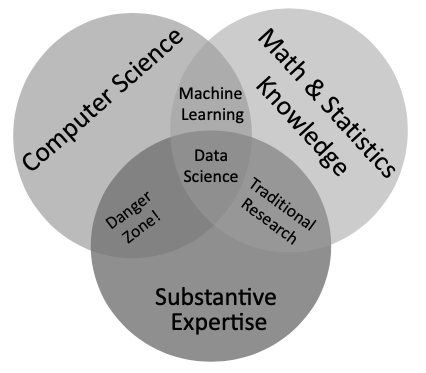
\includegraphics[width=200pt]{images/data-scientist.png}\hspace*{\fill}
  \label{fig:data-scientists}
\end{figure} \\
We distinguish \textbf{two cultures} of Statistical Modeling:
\begin{itemize}
	\item Data modeling (traditional research)
	\item Algorithmic modeling (more like machine learning)
\end{itemize}
\begin{figure}[h!]
 \hfill 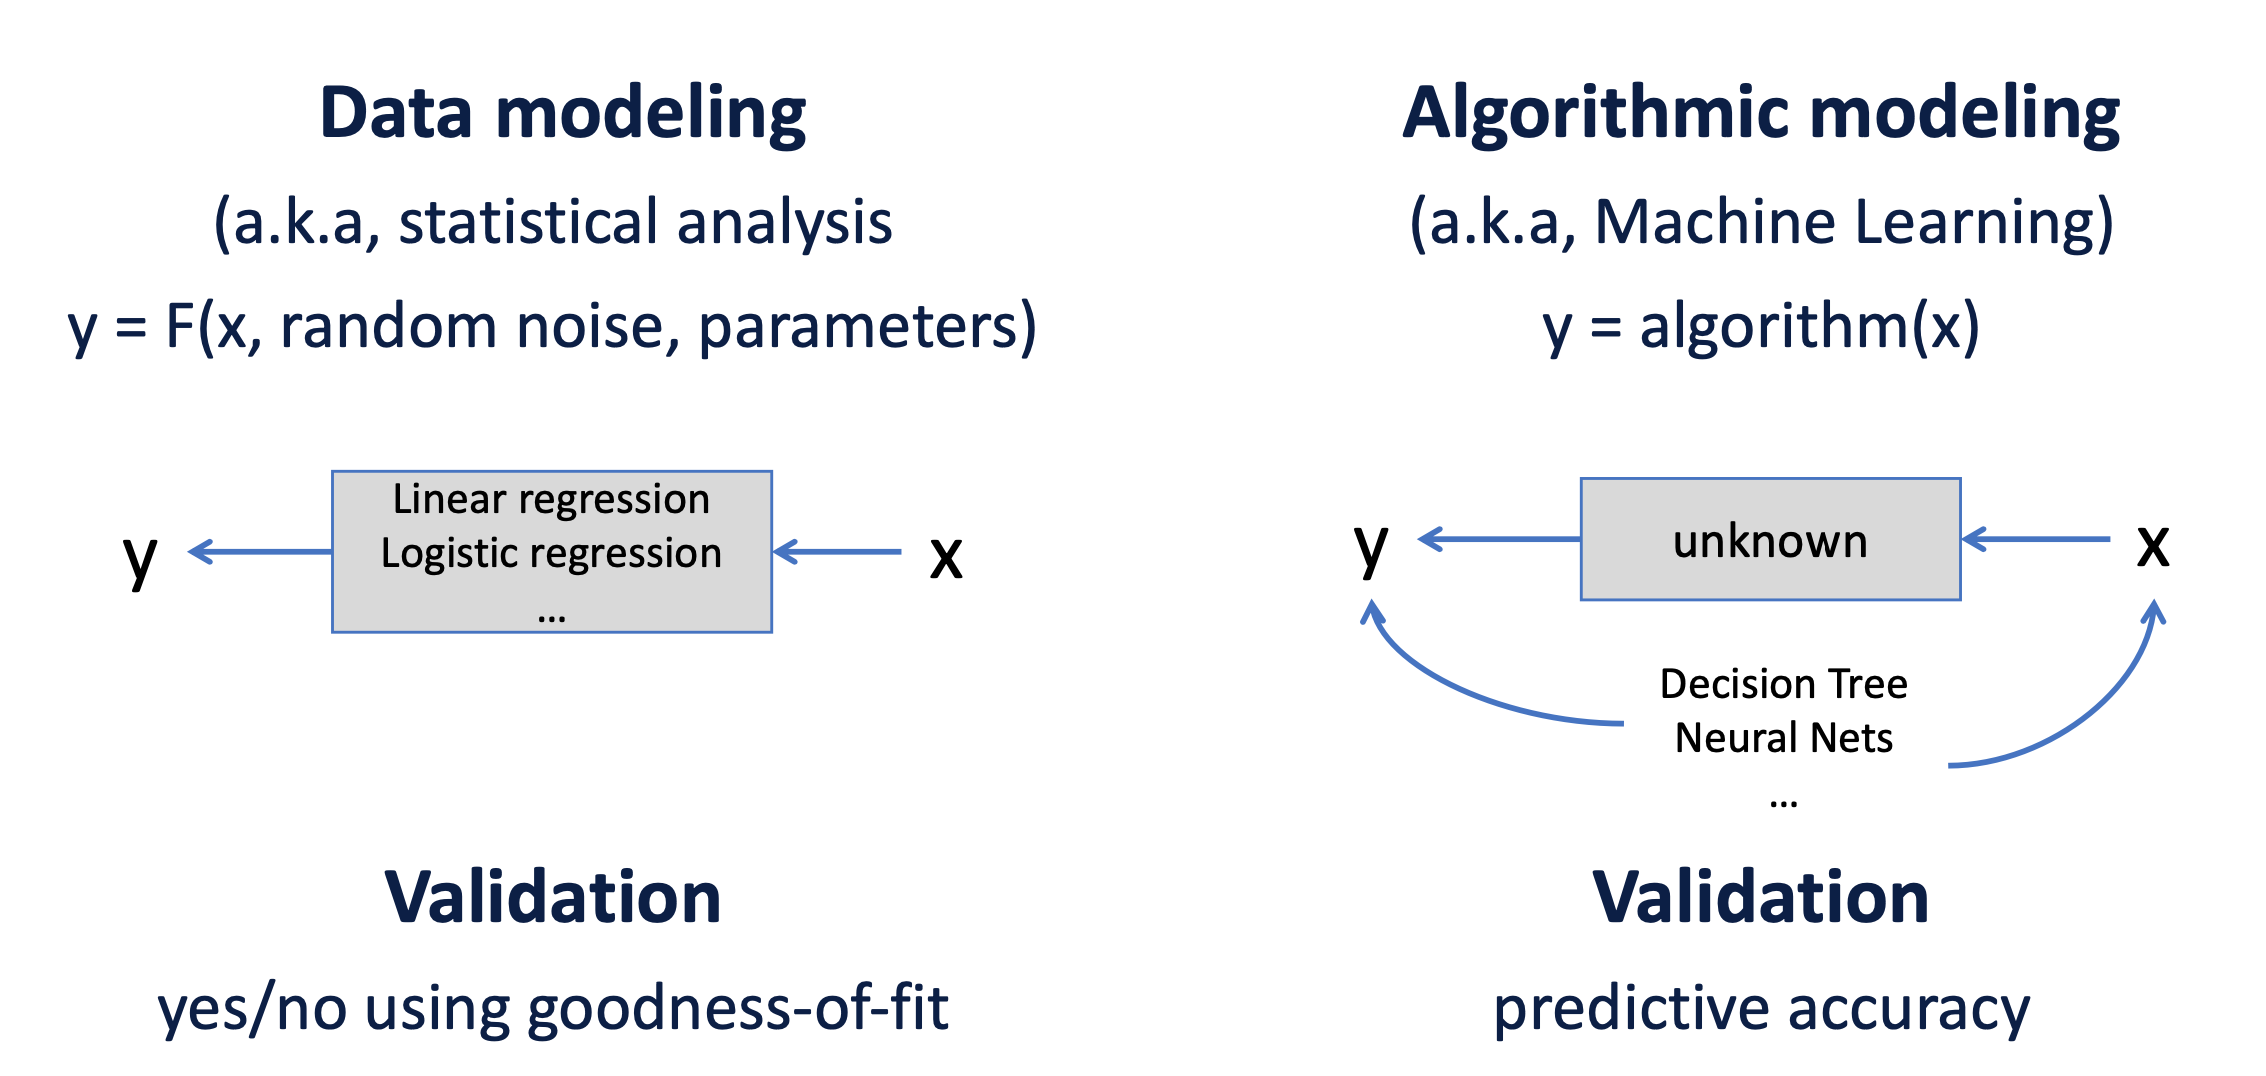
\includegraphics[width=250pt]{images/statistical-modeling.png}\hspace*{\fill}
  \label{fig:statistical-modeling}
\end{figure}
The algorithmic modeling culture starts with data and has two main goals:
\begin{itemize}
	\item Descriptions: describe how nature associates responses to inputs
	\item Predictions: predict response for future input variables
\end{itemize}
\pagebreak
\subsubsection{What's Data Engineering}
Following with the crude oil example, data engineers build "the refinery". 
\center{\textit{"A scientist can discover a new star, but he cannot make one. He would have to ask an engineer to do it for him."} - Gordon Lindsay Glegg} 
\\ \vspace{0.5em} \raggedright
A data engineer is a specialist that \textbf{maintain data and models available and usable} by others (i.e., Data Scientists and Business Analysts). According to Google: "A professional data engineer enables data-driven decision making by collecting, transforming, and publishing data. He should also be able to leverage, deploy, and continuously train pre-existing machine learning models." \\ \vspace{0.5em}
Data engineering purposes a paradigmatic shift, solving problems in new ways.
\begin{figure}[h!]
 \hfill 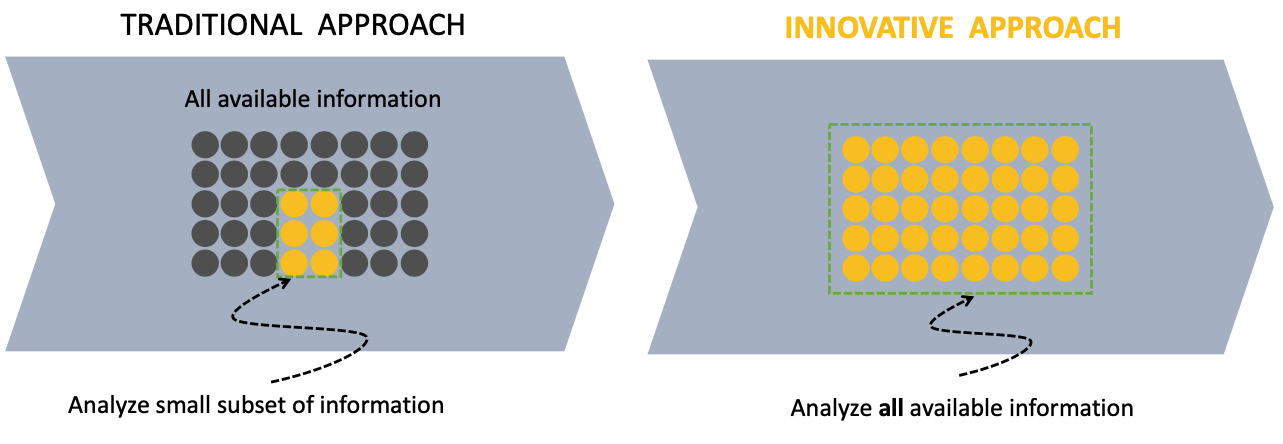
\includegraphics[width=250pt]{images/new-1.png}\hspace*{\fill}
  \label{fig:new1}
\end{figure}
\begin{figure}[h!]
 \hfill 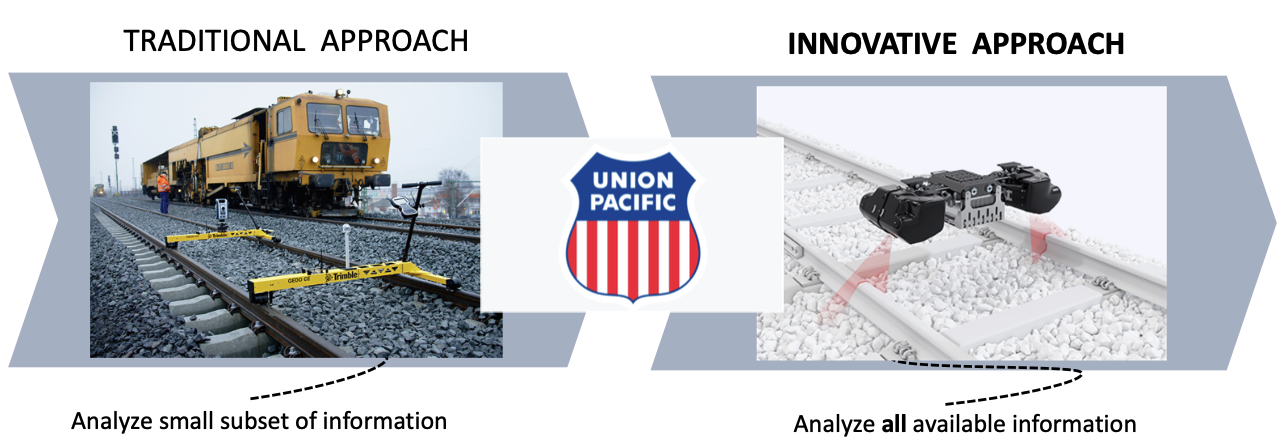
\includegraphics[width=250pt]{images/new-11.png}\hspace*{\fill}
  \label{fig:new11}
  \caption{Instead of looking for the perfect exact data, measure everything and \textbf{leverage more of the data being captured.} With a large enough dataset at some point we reach the same result (Central Limit Theorem).}
  \end{figure}
\begin{figure}[h!]
 \hfill 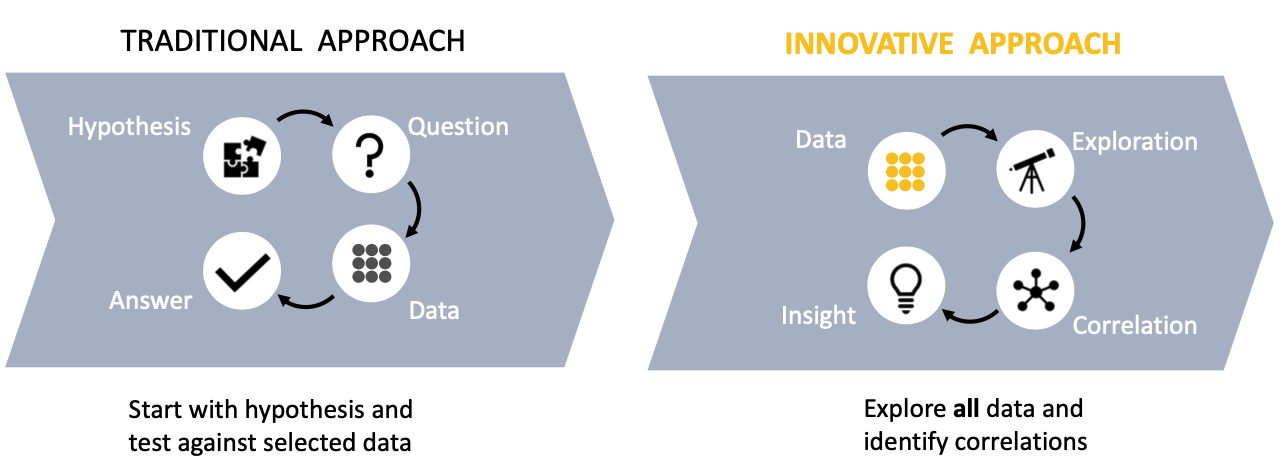
\includegraphics[width=250pt]{images/new-2.png}\hspace*{\fill}
  \label{fig:new2}
  \caption{\textbf{Data-driven exploration looking for correlation.} For instance, your butcher sells both pure meat and semi-prepared dishes because he knows that if you see the variety of products that he prepares and sells, you will probably notice something that you like!}
\end{figure}
 \\
  \pagebreak
\begin{figure}[h!]
 \hfill 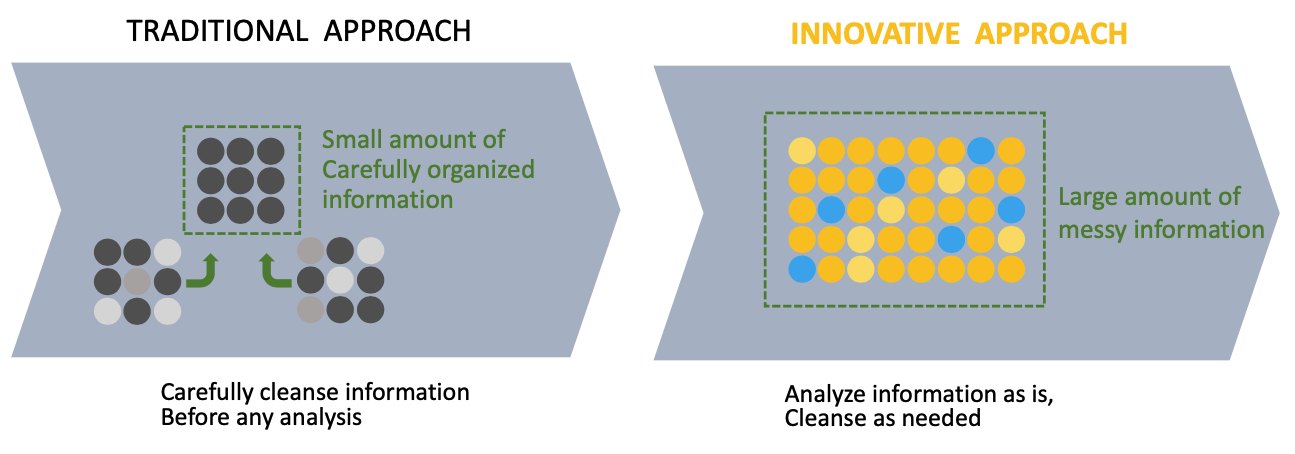
\includegraphics[width=250pt]{images/new-3.png}\hspace*{\fill}
  \label{fig:new3}
\end{figure}
\begin{figure}[h!]
 \hfill 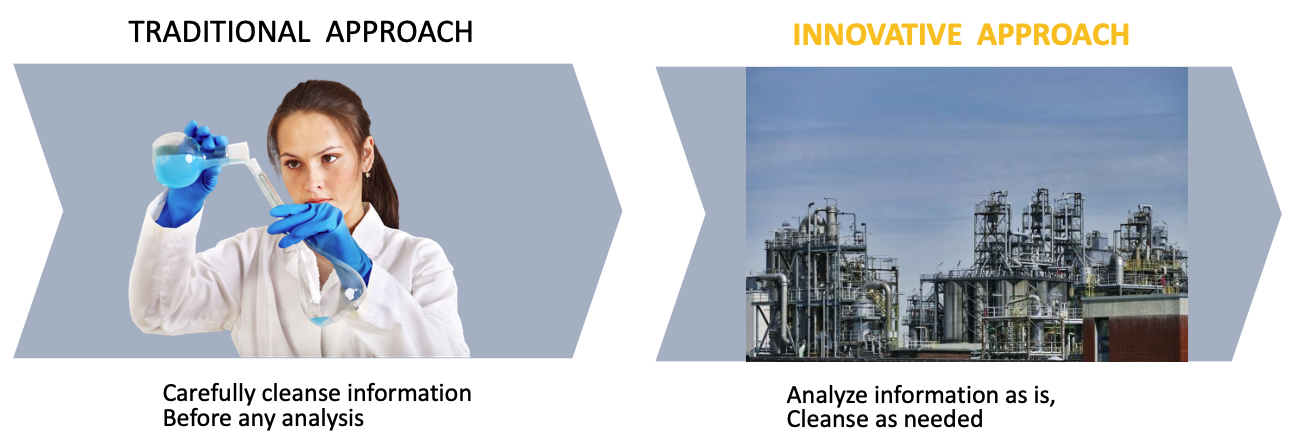
\includegraphics[width=250pt]{images/new-33.png}\hspace*{\fill}
  \label{fig:new33}
  \caption{\textbf{Reduce effort required to leverage data.} If you can do it by hand it is not said that you can do it automatically. Is hard to do things at scale.}
  \end{figure}
  \begin{figure}[h!]
 \hfill 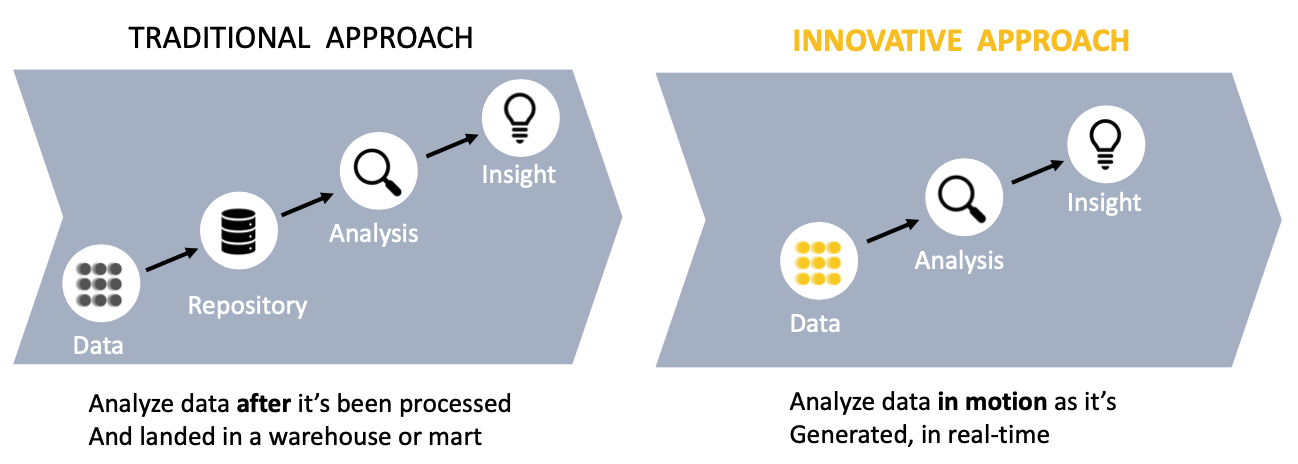
\includegraphics[width=250pt]{images/new-4.png}\hspace*{\fill}
  \label{fig:new4}
\end{figure}
\begin{figure}[h!]
 \hfill 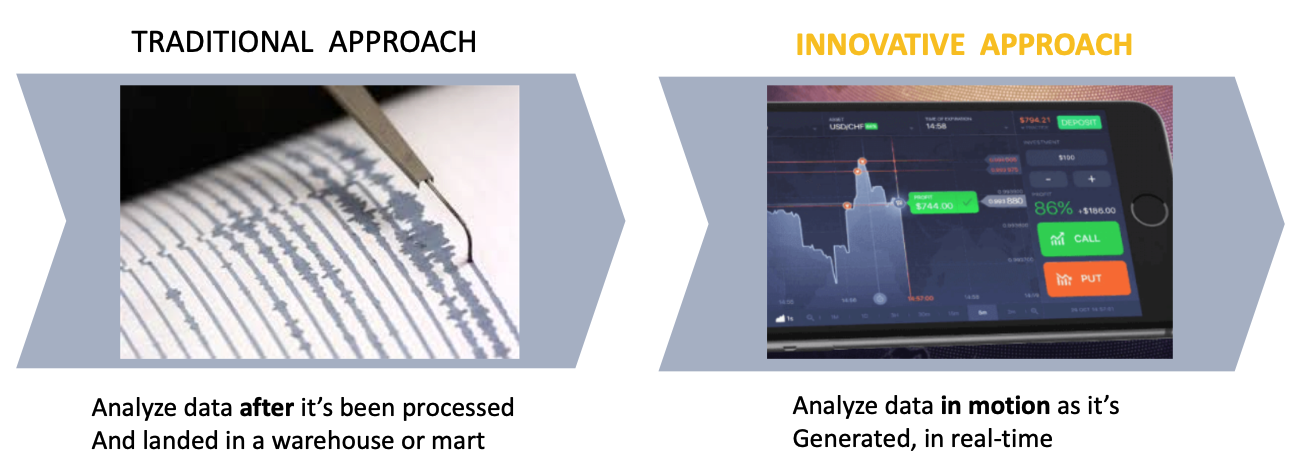
\includegraphics[width=250pt]{images/new-44.png}\hspace*{\fill}
  \label{fig:new44}
  \caption{\textbf{Leverage data as it is captured.}}
  \end{figure}
  The gap is closing thanks to Big Data, Data Science and ... Engineering.
  \begin{figure}[h!]
 \hfill 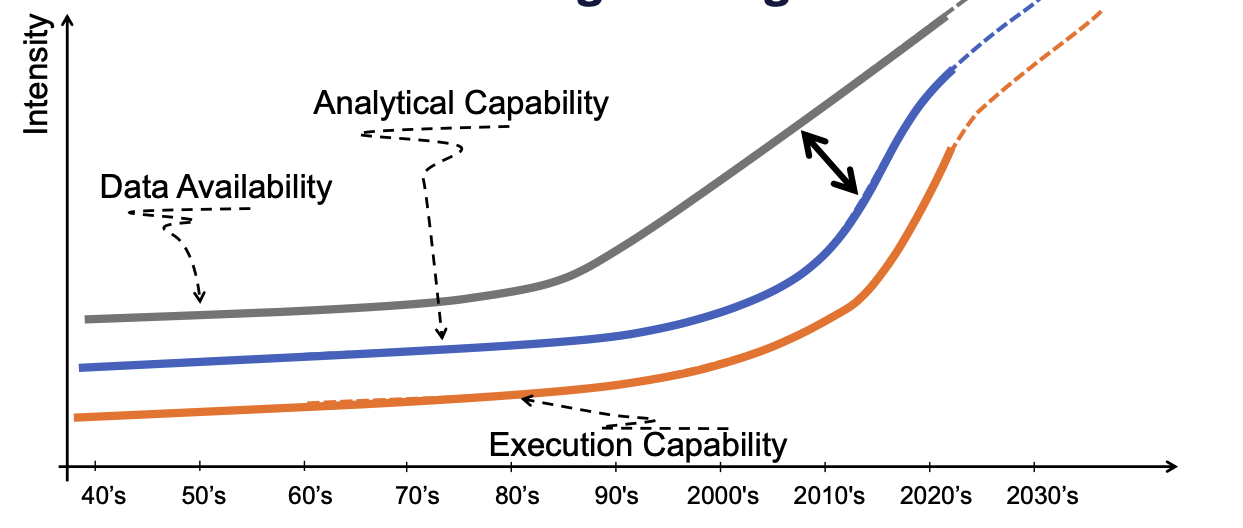
\includegraphics[width=250pt]{images/data-engineering-era.png}\hspace*{\fill}
  \label{fig:data-eng-era}
\end{figure}
\pagebreak
\section{No SQL Intro}
\subsection{Big Data Platforms: Architectures, Features and System}
\subsubsection{Big Data vs Traditional Data}
 \begin{figure}[h!]
 \hfill 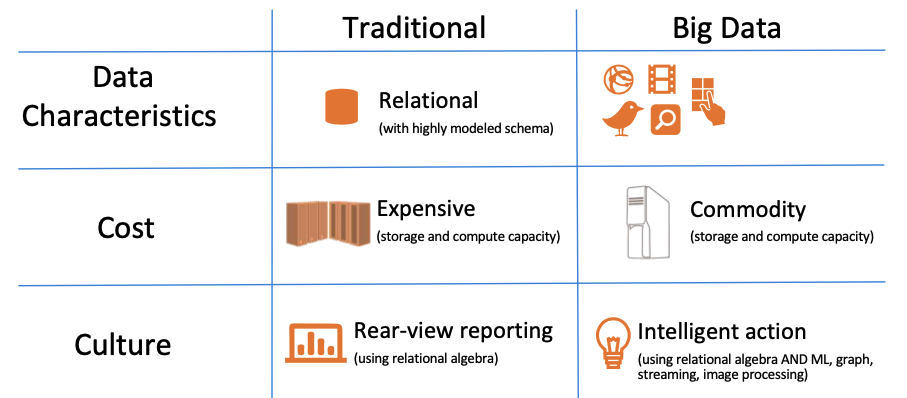
\includegraphics[width=300pt]{images/big-vs-traditional.png}\hspace*{\fill}
  \label{fig:big-vs-traditional}
  \caption{Big Data vs. Traditional Data}
\end{figure}
The first step towards Big Data and flexibility is to adopt a schema-less data storage. Indeed, we don't want to waste time designing complex and fixed schema.
\begin{itemize}
	\item Aggregate-based: key-value, big-table, column-based, document-based
	\item Relationship-based: graph dbs are better than relational!
\end{itemize}
Even in this context we see a paradigmatic shift introduced by Big Data. From \textbf{schema on write} to \textbf{schema-on-read}.
\begin{figure}[h!]
\centering
\begin{minipage}{.5\textwidth}
  \centering
  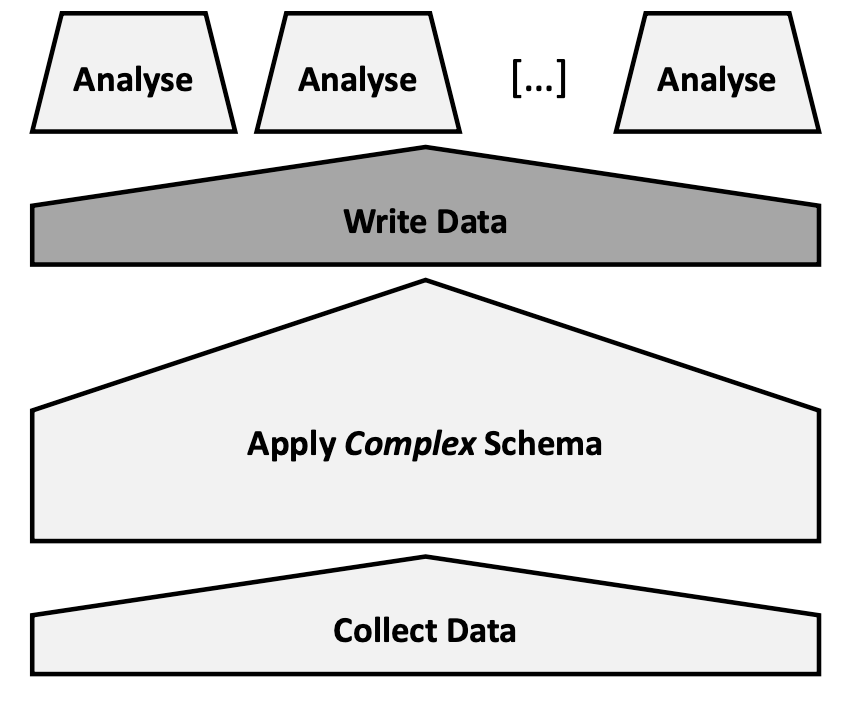
\includegraphics[width=.8\linewidth]{images/schema-on-write}
  \captionof{figure}{\textbf{Schema-on-write}: the rigid and traditional strategy (relational data) in which a complex schema is applied after a long lasting discussing. Here we collect the data from different sources, ensuring that it is compatible with our schema and then we make analysis on that.}
  \label{fig:sow}
\end{minipage}%
\begin{minipage}{.5\textwidth}
  \centering
  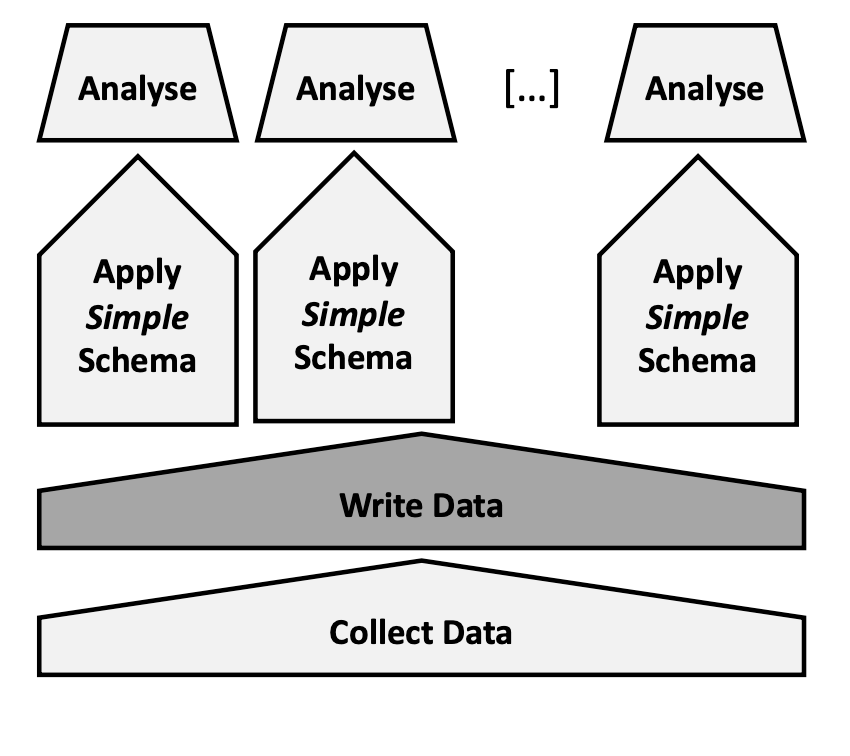
\includegraphics[width=.8\linewidth]{images/schema-on-read}
  \captionof{figure}{\textbf{Schema-on-read}: schema-less approach (document-based data) in which we collect and load data first and ask questions/queries later. All data are kept and the minimal schema for an analysis is applied only when needed. New analysis can then be introduced in any point in time.}
  \label{fig:sor}
\end{minipage}
\end{figure}
\pagebreak
\subsubsection{The Concept of Data Lake}
A Data Lake is a repository in which we store all the possible data that we need in our business. These raw data can be structured or unstructured, without any specific organization and they are there ready to be analyzed when needed. Indeed, there is a specific process that characterized the flow of Big Data into the Data Lake and the various transformation that are applied before analysis and visualization.
\begin{figure}[h!]
\centering
\begin{minipage}{.5\textwidth}
  \centering
  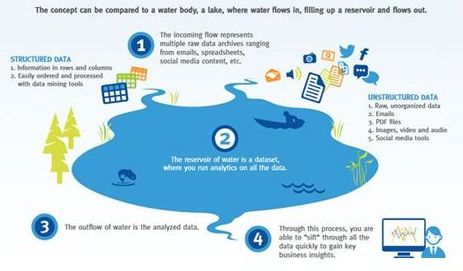
\includegraphics[width=.9\linewidth]{images/data-lake}
  \captionof{figure}{Data lake}
  \label{fig:data-lake}
\end{minipage}%
\begin{minipage}{.5\textwidth}
  \centering
  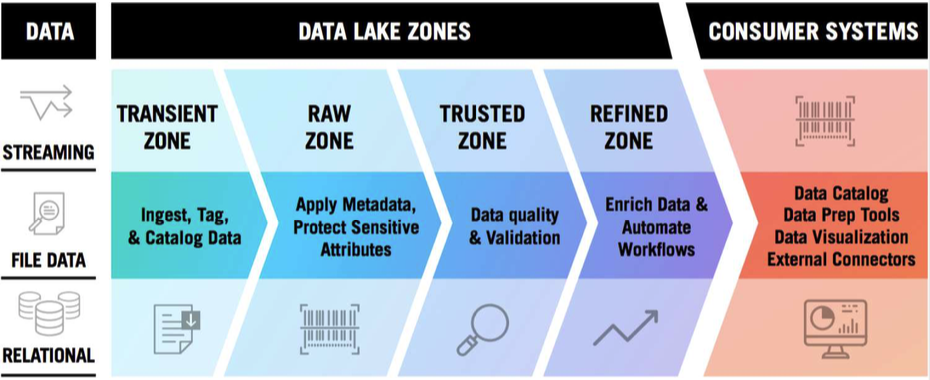
\includegraphics[width=.9\linewidth]{images/data-lake-process}
  \captionof{figure}{Data Lake in process}
  \label{fig:data-lake-process}
\end{minipage}
\end{figure}  \\
\textbf{Data Ingestion} is the process of importing, transferring and loading data for storage and later use. It involves loading data from a variety of sources. It can involve altering and modification of individual files to fit into a format that optimizes the storage. For instance, in Big Data small files are concatenated to form files of 100s of MBs and large files are broken down in files of 100s of MBs. \\
\textbf{Data Wrangling}: the process of cleansing "raw" data and transforming raw it into data that can be analysed to generate valid actionable insight. It includes understanding, cleansing, augmenting and shaping data. The results is data in the best format (e.g., columnar) for the analysis to perform.
\begin{figure}[h!]
 \hfill 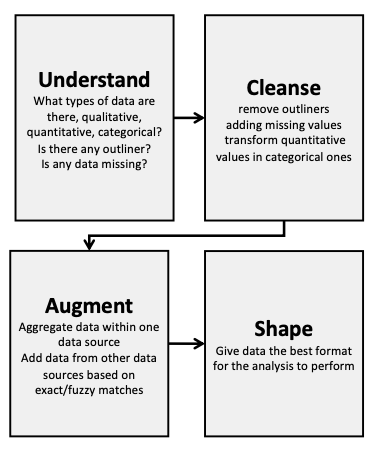
\includegraphics[width=200pt]{images/data-wrangling.png}\hspace*{\fill}
  \label{fig:data-wrangling}
  \caption{Data Wrangling}
\end{figure}
\pagebreak
\subsubsection{Scalability}
Adding data to a system may degrade its performances.
\begin{itemize}
	\item \textbf{"Traditional" SQL system scale vertically}: when the machine, where the SQL system runs, no longer performs as required, the solution is to \textbf{buy a better machine} (with more RAM, more cores and more disk).
	\item \textbf{Big Data solutions scale horizontally}: when the machines, where the big data solution runs, no longer performs as required, the solution is \textbf{to add another machine.}
\end{itemize}
\begin{figure}[h!]
\centering
\begin{minipage}{.5\textwidth}
  \centering
   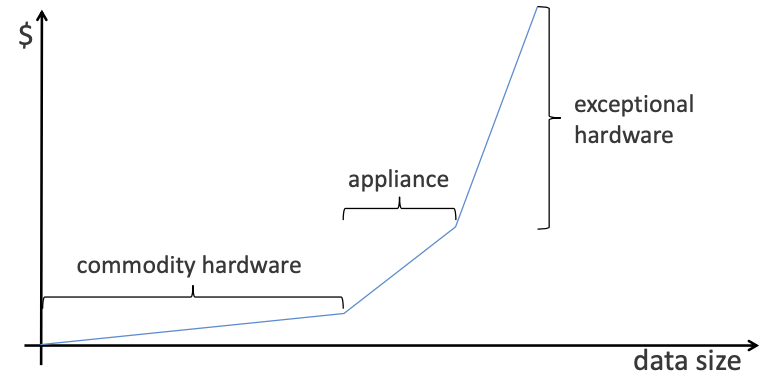
\includegraphics[width=.9\linewidth]{images/vertical-scalability}
  \captionof{figure}{Vertical Scalability}
  \label{fig:vertical}
\end{minipage}%
\begin{minipage}{.5\textwidth}
  \centering
  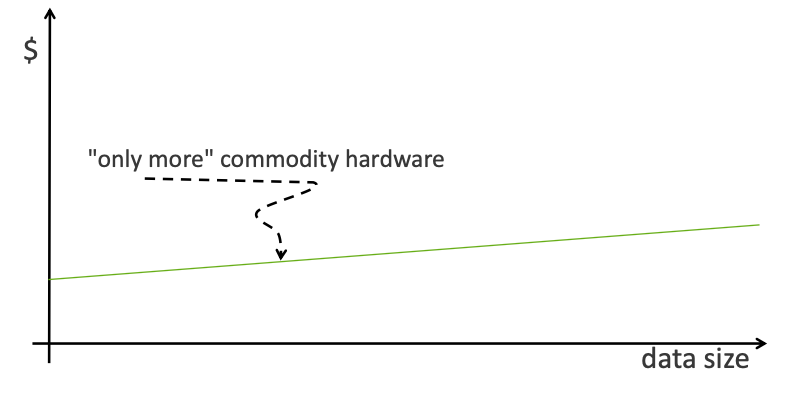
\includegraphics[width=.9\linewidth]{images/horizontal-scalability}
  \captionof{figure}{Horizontal Scalability}
  \label{fig:horizontal}
\end{minipage}
\end{figure} 
\begin{figure}[h!]
 \hfill 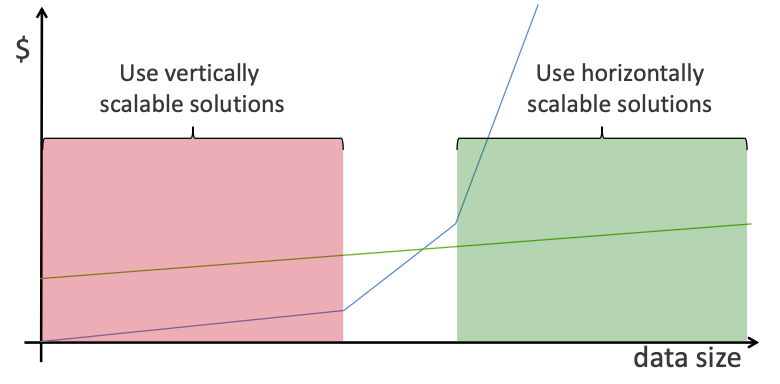
\includegraphics[width=200pt]{images/vertical-vs-horizontal.png}\hspace*{\fill}
  \label{fig:vertical-vs-horizontal}
  \caption{Vertical (Exponential) vs Horizontal (Linear) growth}
\end{figure}

\begin{figure}[h!]
\centering
\begin{minipage}{.5\textwidth}
  \centering
   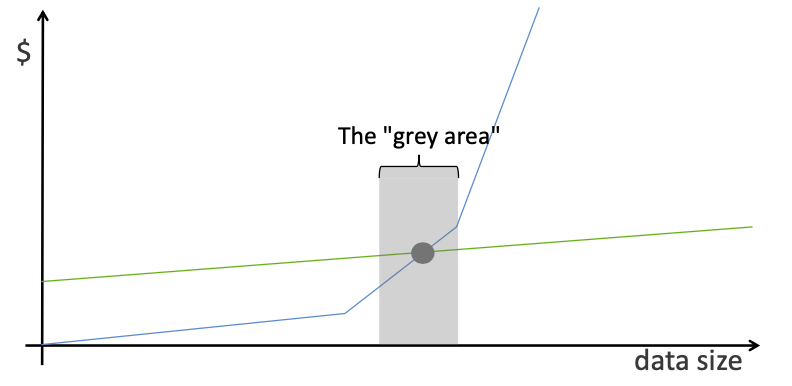
\includegraphics[width=.9\linewidth]{images/grey-area}
  \captionof{figure}{The space within vertical (blue) and horizontal (red) scalable solution. On the left we see an high price gap between the blue and the red line for which the preferred solution is the vertical scalability. On the right is the contrary: the price is growing faster on the blue line while the horizontal scalable solution price is growing linearly.}
  \label{fig:grey-area}
\end{minipage}%
\begin{minipage}{.5\textwidth}
  \centering
  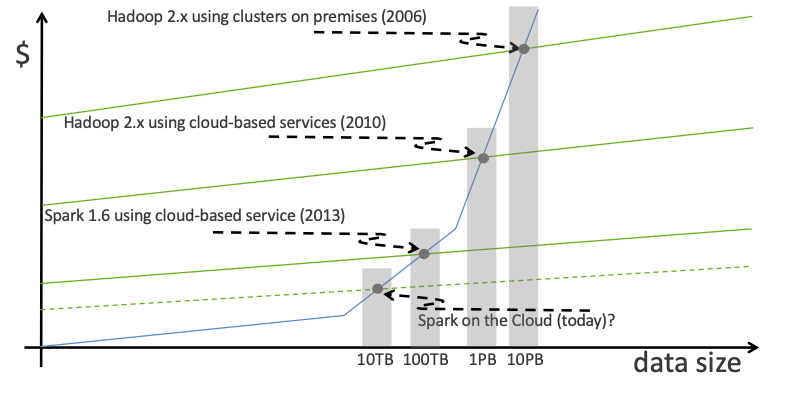
\includegraphics[width=.9\linewidth]{images/grey-area-in-time}
  \captionof{figure}{The grey area moves in time. As a result, we can see that horizontal scalability now makes sense when we have to deal with 10TB of data.}
  \label{fig:grey-area-in-time}
\end{minipage}
\end{figure} 
\pagebreak
\subsection{ACID vs. BASE and SQL vs. NoSQL}
\subsubsection{Transactional Properties}
\uline{Definition of Transaction}: An elementary unit of work performed by an application. Each transaction is encapsulated within two commands: \textbf{begin transaction} (bot) and \textbf{end transaction} (eot).
\\ Within a transaction of the commands below is executed \textit{exactly once}:
\textcolor{red}{commit work} (commit) and \textcolor{red}{rollback work} (abort). \\
A \textcolor{red}{Transactional System} (OLTP) is a system capable of providing the definition and execution of transactions on behalf of multiple, concurrent applications.
\begin{figure}[h!]
 \hfill 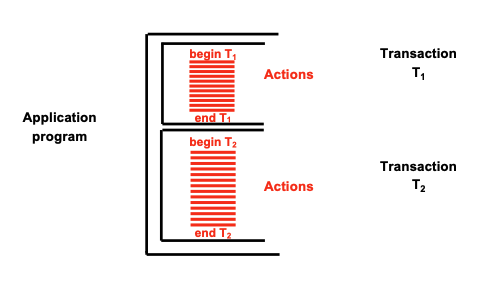
\includegraphics[width=200pt]{images/transactions.png}\hspace*{\fill}
  \label{fig:transactions}
  \caption{Application and Transactions}
\end{figure}
\begin{figure}[h!]
\centering
\begin{minipage}{.5\textwidth}
  \centering
   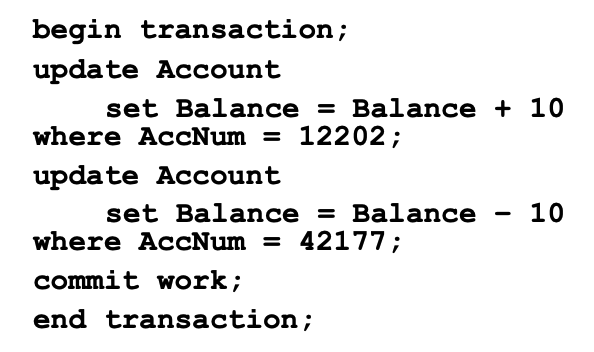
\includegraphics[width=.7\linewidth]{images/transaction-ex}
  \captionof{figure}{Transaction example}
  \label{fig:t1}
\end{minipage}%
\begin{minipage}{.5\textwidth}
  \centering
  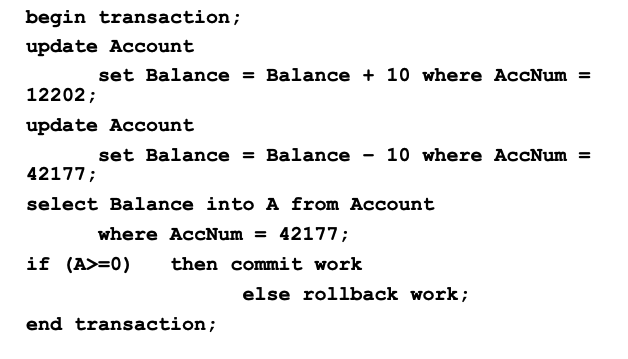
\includegraphics[width=.7\linewidth]{images/transaction-ex2}
  \captionof{figure}{Another Transaction example with rollback}
  \label{fig:t2}
\end{minipage}
\end{figure} 
\paragraph{ACID Properties of Transactions}
A transaction is a unit of work enjoying the following properties:
\begin{itemize}
	\item \textbf{Atomicity}: a transaction is an atomic transformation from the initial state to the final state. Three possible behaviors:
	\begin{itemize}
		\item Commit work: SUCCESS
		\item Rollback work or error prior to commit: UNDO
		\item Fault after commit: REDO
	\end{itemize}
	\textcolor{red}{Abort-rollback restart} and \textcolor{red}{Commit protocols}
	\item \textbf{Consistency}: the transaction satisfies the integrity of constraints on data. As a consequence, if the initial state is consistent, then the final state is also consistent. \textcolor{red}{Integrity checking of DBMS}
	\item \textbf{Isolation}: a transaction is not affected by the behavior of other, concurrent transactions. As a consequence, its intermediate states are not exposed and the "domino effect" is avoided. \textcolor{red}{Concurrency control}
	\item \textbf{Durability}: the effect of a transaction that has successfully committed will last "forever" independently of any system fault. \textcolor{red}{Recovery management}
\end{itemize}
These properties characterizes relational DBMS and for this reason such systems offer very expensive and rigid solutions.
\subsubsection{CAP Theorem}
It is impossible for a \uline{distributed computer system} to simultaneously provide all three of the following guarantees:
\begin{itemize}
	\item \textbf{Consistency}: all nodes see the same data at the same time
	\item \textbf{Availability}: node failures do not prevent other survivors from continuing to operate (a guarantee that every request receives a response about whether it succeeded or failed)
	\item \textbf{Partition tolerance}: the system continues to operate despite arbitrary partitioning due to network failures (e.g., message loss)
\end{itemize}
A distributed system can satisfy any two of these guarantees at the same time but not all three. \\ 
In a distributed system, a network (of networks) is inevitable (by definition). We can't avoid to deal with partition tolerance, we need to cover that. Indeed. Failures can, and will, occur to a networked system. Then, the only option left is choosing between \textbf{C}onsistency and \textbf{A}vailability. This because CA doesn't make any sense, because is what traditional centralized database are guaranteeing. \\
We have two solutions:
\begin{itemize}
	\item AP: a partitioned node returns
	\begin{itemize}
		\item a correct value, if in a consistent state;
		\item a timeout error or an error, otherwise;
		\item e.g., DynamoDB, CouchDB, and Cassandra
	\end{itemize}
	\item CP: a partitioned note returns the most recent version of the data, which could be stale
	\begin{itemize}
		\item e.g., MongoDB, Redis, AppFabric Caching and MemcacheDB
	\end{itemize}
\end{itemize}
By the way, Consistency and Availability should not necessarily be guaranteed in a mutually exclusive manner, but possibly by partial accomodation of both. We need to do some trade-off analyses.
\begin{figure}[h!]
\centering
\begin{subfigure}{.5\textwidth}
  \centering
  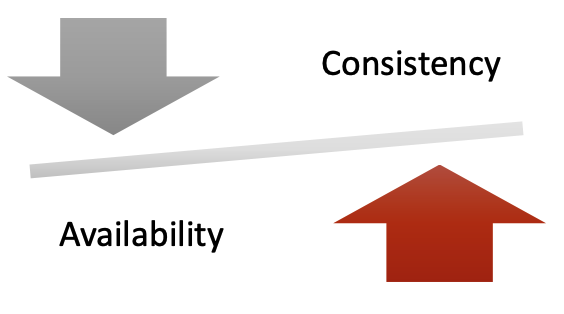
\includegraphics[width=.5\linewidth]{images/availability-vs-consistency}
  \caption{\textbf{Consistency vs Availability}}
  \label{fig:ca}
\end{subfigure}%
\begin{subfigure}{.5\textwidth}
  \centering
  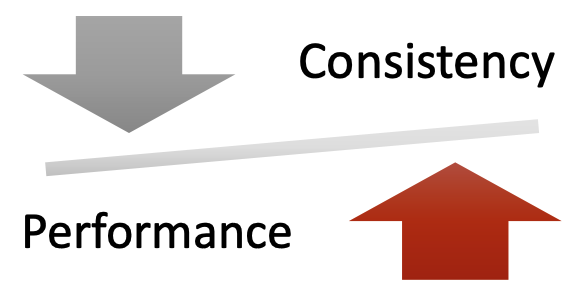
\includegraphics[width=.5\linewidth]{images/performance-vs-consistency}
  \caption{\textbf{Consistency vs Performance}}
  \label{fig:cp}
\end{subfigure}
\caption{We need to choose between consistency and availability. According to the use case scenario, we can choose which one to favour. For example, \uline{consistency should be preferred in banking applications}, where the transactions of money should be carefully saved and stored in a rigid flow to allow the correct functioning of the system. While almost \uline{all the social media apps or streaming platforms may concentrate on availability} since if some data in the communication is lost or some user content are not presented in the latest version, the app can continue providing the service without creating any big issues to the user. Talking about \uline{performance}, high consistency usually results in low performance while high performance results in low consistency.}
\label{fig:cap}
\end{figure}
\begin{figure}[h!]
 \hfill 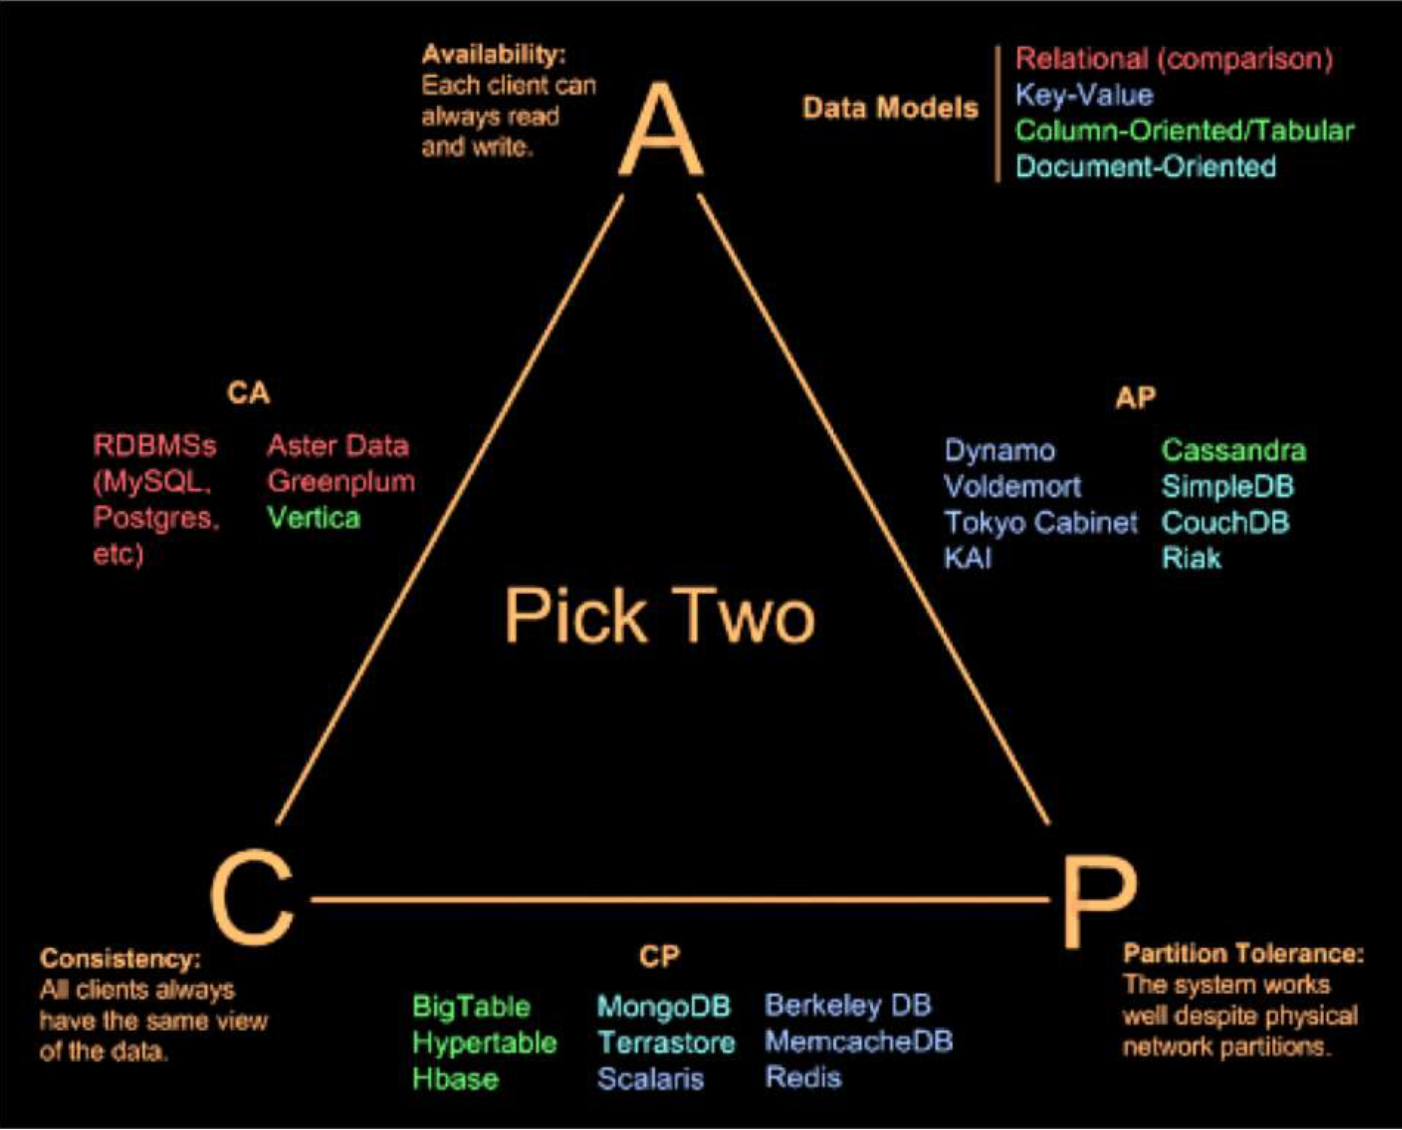
\includegraphics[width=300pt]{images/cap-theorem.png}\hspace*{\fill}
  \label{fig:cap-theorem}
  \caption{Visual Guide to CAP Theorem}
\end{figure} \\ \pagebreak
\subsubsection{ACID vs. BASE properties}
\textbf{SQL databases:}
\begin{itemize}
	\item Structured query language
	\item Traditional relational databases (unique keys, single valued, no update/insertion/deletion anomalies)
	\item Well structured data
	\item ACID properties should hold
\end{itemize}
\textbf{NoSQL (Not Only SQL) databases:}
\begin{itemize}
	\item Triggered by the storage needs of Web 2.0 companies such as Facebook, Google and Amazon.com
	\item Not necessarily well structured - e.g., pictures, documents, web page description, video clips, etc.
	\item \uline{ACID properties may not hold}, but this does not mean that there are no properties at all (there are new properties)
	\item focuses on availability of data even in the presence of multiple failures
	\item spread data across many storage systems with a high degree of replication
\end{itemize}
\textbf{BASE} properties are much weaker properties w.r.t. to ACID ones. The rationale behind them is that it's ok to use stale data and it's okay to give approximate answers. 
\begin{itemize}
	\item \uline{\textbf{B}asic \textbf{A}vailability}: fulfill request, even in partial consistency. Basic functionalities are always provided.
	\item \uline{\textbf{S}oft State}: abandon the consistency requirements of the ACID model pretty much completely.
	\item \uline{\textbf{E}ventual consistency}: at some point in the future, data will converge to a consistent state; delayed consistency, as opposed to immediate consistency of the ACID properties.
	\begin{itemize}
		\item purely a liveness guarantee (reads eventually return the requested value);
		\item no safety guarantees, i.e., an eventually consistent system can return any value before it converges
	\end{itemize}
\end{itemize}
\subsubsection{The NoSQL World}
\center{\textit{Google, Amazon, Facebook, and DARPA all recognized that \textbf{when you scale systems large enough, you can never put enough iron in one place to get the job done} (and you wouldn’t want to, to prevent a single point of failure).
Once you accept that you \textbf{have a distributed system, you need to give up consistency or availability}, which the fundamental transactionality of traditional RDBMSs cannot abide.} - Cedric Beust}
\\ \raggedright \vspace{0.5em}
The acronym \textbf{NoSQL} was first used in 1998 by Carlo Strozzi while naming his lightweight, open-source "relational" database that did not use SQL. NoSQL term was used to say that he was not using an SQL interface. \\ 
The term was then reintroduced in early 2009, when Eric Evans and Johan Oskarsson used it to describe non-relational databases (which are often referred to as SQL systems). In that case the term was meaning "not only SQL" to emphasize the fact that some systems might even support SQL-like query languages.
\paragraph{\uline{Kind of NoSQL}}
NoSQL solutions fall into two major areas:
\begin{itemize}
	\item \textbf{Key/Value} or "the big hash table"
	\begin{itemize}
		\item Amazon S3 (Dynamo)
		\item Voldemort
		\item Scalaris
		\item Memcache DB
		\item Azure Table Storage
		\item Redis
		\item Riak
	\end{itemize}
	\item \textbf{Schema-less}
	\begin{itemize}
		\item Cassandra (column-based)
		\item CouchDB (document-based)
		\item Neo4J
		\item HBase
	\end{itemize}
\end{itemize}
\paragraph{\uline{Different types of NoSQL}}
\begin{itemize}
	\item \textbf{Key-Value Store}: A key that refers to a payload (actual content /data). \\ \textit{MemcacheDB, Azure Table Storage, Redis}
	\item \textbf{Column Store}: column data is saved together, as opposed to row data. Super useful for data analytics. \\ \textit{Hadoop, Cassandra, Hypertable}
	\item \textbf{Document / XML / Object Store}: key (and possibly other indexes) point at serialized object. DB can operate against values in document. \\ \textit{MongoDB, CouchDB, RavenDB}
	\item \textbf{Graph Store}: nodes are stored independently, and the relationship between nodes (edges) are stored with data. \\ \textit{Neo4J}
\end{itemize}
\begin{figure}[h!]
 \hfill 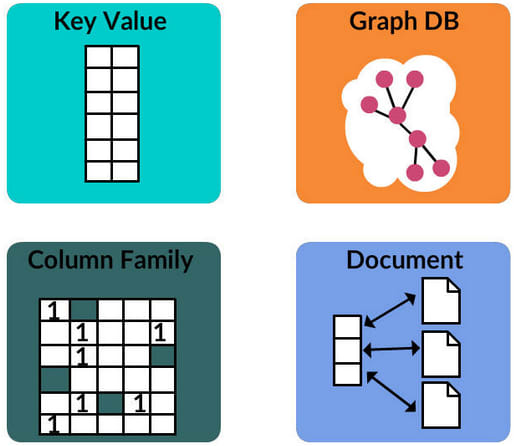
\includegraphics[width=150pt]{images/nosqltypes.jpeg}\hspace*{\fill}
  \label{fig:nosqltypes}
  \caption{NoSQL types}
\end{figure} 
\pagebreak
Most of NoSQL databases are open source projects started and/or supported by the most famous companies in the world, cause they needed to create custom solutions to improve their performance.
\begin{itemize}
	\item Google $\rightarrow$ BigTable, LevelDB
	\item LinkedIn $\rightarrow$ Voldemort
	\item Facebook $\rightarrow$ Cassandra
	\item Twitter $\rightarrow$ Hadoop/HBase, FlockDB, Cassandra
	\item Netflix $\rightarrow$ SimpleDB, Hadoop/HBase, Cassandra
	\item CERN $\rightarrow$ CouchDB
\end{itemize}
This is a big shift from traditional SQL-based produced by companies such as Oracle, IBM and Microsoft. They are still selling traditional, relational and transactional DBMS. Indeed, their projects are not open source. \\ \vspace{1em}
In conclusion, there is no general answer to whether your application needs an ACID versus BASE consistency model. Given BASE's loose consistency, developers need to be more \textbf{knowledgeable and rigorous about consistent data} if they choose a BASE store for their application. Planning around BASE limitations can sometimes be a major disadvantage when compared to the simplicity of ACID transactions. A fully ACID database is the perfect fit for use cases where data reliability and consistency are essential.
\begin{figure}[h!]
 \hfill 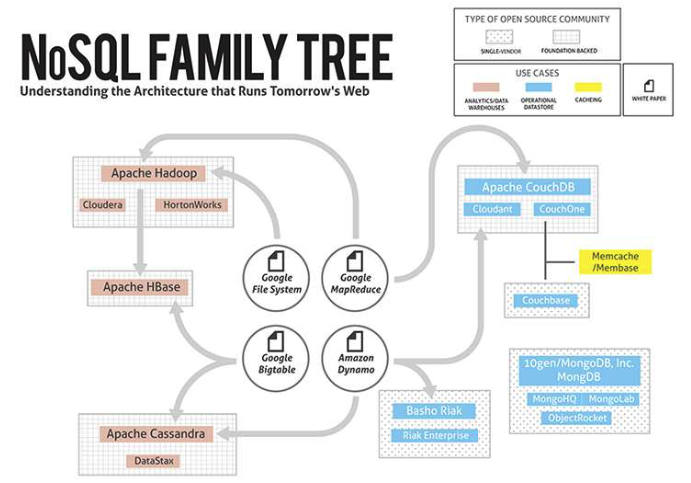
\includegraphics[width=350pt]{images/nosqlfamtree.png}\hspace*{\fill}
  \label{fig:nosqlfamtree}
\end{figure} 
\section{Graph DB}
Graph databases address one of the great macroscopic business trends of today: leveraging complex and dynamic relationships in highly connected data to generate insight and competitive advantage. For data of any significant size or value, graph databases are the best way to represent and query connected data. Connected data is data whose interpretation and value requires us first to understand the ways in which its constituent elements are related. \nline
Although large corporations realized this some time ago and began creating their own proprietary graph processing technologies, we are now in an era where that technology has rapidly become democratized. Today, general-purpose graph databases are a reality, enabling mainstream users to experience the benefits of connected data without having to invest in building their own graph infrastructure.
\nline
Graph theory was pioneered by Euler in the 18th century, and has been actively researched and improved by mathematicians, sociologists, anthropologists, and other practitioners ever since. However, it is only in the past few years that graph theory and graph thinking have been applied to information management. In that time, graph databases have helped solve important problems in the areas of social networking, master data management, geospatial, recommendations, and more. This increased focus on graph databases is driven by two forces: by the massive commercial success of companies such as Facebook, Google, and Twitter, all of whom have centered their business models around their own proprietary graph technologies; and by the introduction of general-purpose graph databases into the technology landscape.
\subsection{Graph Theory}
Formally, a graph is just a collection of \textit{vertices} and \textit{nodes} $-$ or, in other words, a set of \textit{nodes} and the \textit{relationships} that connect them. Graphs represent entities as nodes and the ways in which those entities relate to the world as relationships. This general-purpose expressive structure allows us to model all kinds of scenarios that we can imagine.
Indeed, graphs are extremely useful in understanding a wide diversity of datasets in fields such as science, government, and business. \\ For example, Twitter's data is represented as a graph. In Figure 25 we ee a small network of Twitter users. Each node is labeled \textit{User}, indicating its role in the network. These nodes are then connected with relationships, which help further establish the semantic context: namely, that Billy follows Harry, and that Harry, in turn, follows Billy. Ruth and Harry likewise follow each other, but sadly, although Ruth follows Billy, Billy hasn't (yet) reciprocated.
\begin{figure}[h!]
 \hfill 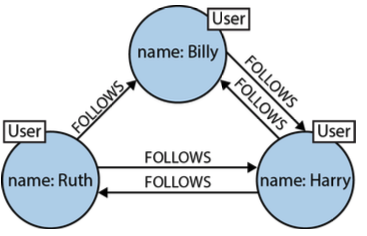
\includegraphics[width=180pt]{images/twitter-graph.png}\hspace*{\fill}
  \caption{A small social graph}
\end{figure} \\
Of course, Twitter’s real graph is hundreds of millions of times larger than the example in Figure 25, but it works on precisely the same principles. In Figure 26 we’ve expanded the graph to include the messages published by Ruth. \pagebreak
\begin{figure}[h!]
 \hfill 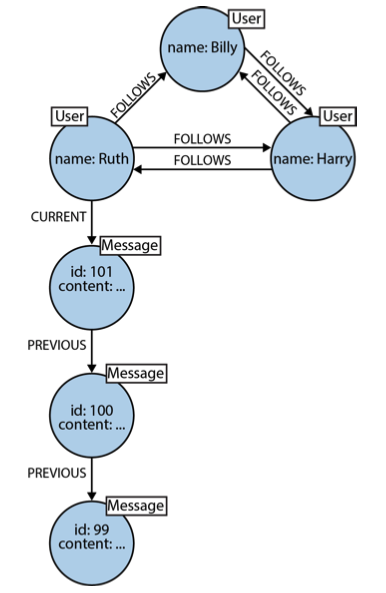
\includegraphics[width=150pt]{images/twitter-graph2.png}\hspace*{\fill}
  \caption{Publishing messages}
\end{figure} \\
Though simple, Figure 26 shows the expressive power of the graph model. It’s easy to see that Ruth has published a string of messages. Her most recent message can be found by following a relationship marked CURRENT. The PREVIOUS relationships then create Ruth’s timeline. \nline
In discussing Figure 26 we’ve also informally introduced the most popular form of graph model, the \textbf{labeled property graph}. A labeled property graph has the following characteristics:
\begin{itemize}
	\item It contains nodes and relationships
	\item Nodes contain properties (key-value pairs)
	\item Nodes can be labeled with one or more labels
	\item Relationships are named and directed, and always have a start and end node
	\item Relationships can also contain properties
\end{itemize}
\subsubsection{Useful definitions}
\textbf{Vertex}
\begin{itemize}
	\item Basic element
	\item Drawn as a node or a dot
	\item Vertex set of G is usually denoted by $V(G)$, or $V$
\end{itemize}
\textbf{Edge}
\begin{itemize}
	\item A set of two elements
	\item Drawn as a line connecting two vertices, called end vertices, or endpoints
	\item The edge set of G is usually denoted by $E(G)$, or $E$
\end{itemize} \pagebreak
\begin{figure}[h!]
 \hfill 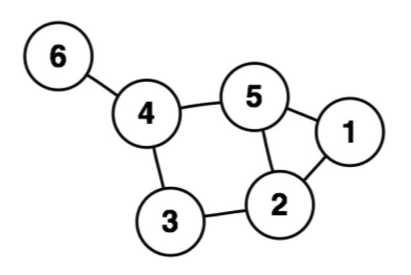
\includegraphics[width=150pt]{images/graph-example.png}\hspace*{\fill}
  \caption{$V:= \{1,2,3,4,5,6\} - E: \{ \{1,2\},\{1,5\},\{2,3\},\{2,5\},\{3,4\},\{4,5\},\{4,6\}\}$}
\end{figure}
\textbf{Simple graphs}: simple graphs are graphs without multiple edges or self-loops.
\nline
\textbf{Path}: a path is a sequence of vertices such that there is an edge from each vertex to its successor. A path is \uline{simple} if each vertex is distinct.
\begin{figure}[h!]
 \hfill 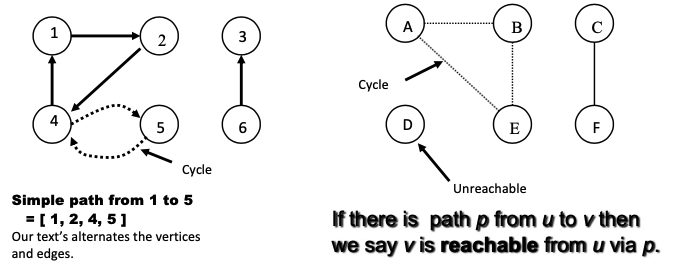
\includegraphics[width=250pt]{images/graph-path.png}\hspace*{\fill}
  \caption{Graph path and reachability}
\end{figure} \\
\textbf{Cycle}: a path from a vertex to itself is called cycle. A graph is called \uline{cyclic} if it contains a cycle; otherwise it is called \uline{acyclic}
\begin{figure}[h!]
 \hfill 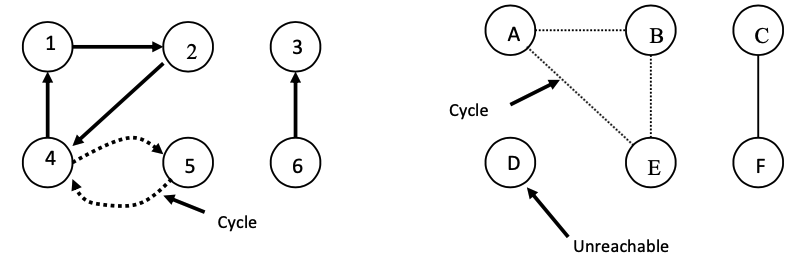
\includegraphics[width=220pt]{images/graph-cycle.png}\hspace*{\fill}
  \caption{Graph cycle}
\end{figure} \\
\textbf{Connectivity}: a graph is \uline{connected} if and only if
\begin{itemize}
	\item you can get from any node to any other by following a sequence of edges OR
	\item any two nodes are connected by a path
\end{itemize}
A directed graph is \uline{strongly connected} if there is a directed path from any node to any other node. \nline
\textbf{Sparse/Dense}
\begin{itemize}
	\item A graph is \uline{sparse} if $|E| \approx |V|$ (same number of edges and vertices $\rightarrow$ very few connections)
	\item A graph is \uline{dense} if $|E| \approx |V|^2$ (graph full of connections $\rightarrow$ with $n$ vertices, there can be a max of $n(n-1)$ edges)
\end{itemize}
 \pagebreak
\textbf{Weighted Graph}: is a graph for which each edge has an associated \uline{weight}, usually given by a weight function $w:E\rightarrow R$.
\begin{figure}[h!]
 \hfill 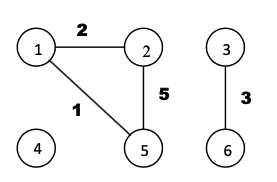
\includegraphics[width=150pt]{images/graph-weight.png}\hspace*{\fill}
  \caption{For example, in a GPS navigator we could use weight to specify duration, distance or traffic. The shortest path between two nodes is then calculated selecting the edges with the lowest weight.}
\end{figure}  \\
\textbf{Directed Graph}: edges have directions and the arch can be followed only in that direction
\nline
\textbf{Bipartite Graph}: V can be partitioned into 2 sets $V_1$ and $V_2$ such that $(u,v) \in E$ implies:
\begin{itemize}
	\item either $u \in V_1$ and $v \in V_2$
	\item OR $v \in V_1$ and $u \in V_2$
\end{itemize}
\begin{figure}[h!]
 \hfill 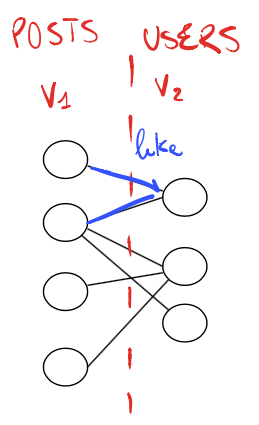
\includegraphics[width=120pt]{images/bipartite-graph.png}\hspace*{\fill}
  \caption{Nodes in $V_1$ connects only with nodes in $V_2$ (usually those are different categories of nodes e.g., Users and Posts)}
\end{figure} 
\textbf{Complete Graph}: denoted by $K_n$, in a complete graph every pair of vertices are adjacent with a total of $n(n-1)$ edges.
\begin{figure}[h!]
 \hfill 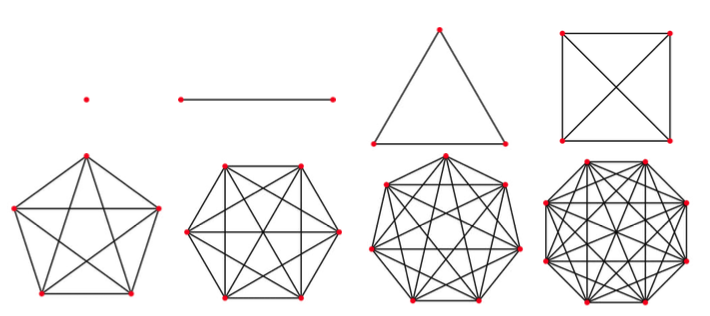
\includegraphics[width=160pt]{images/complete-graph.png}\hspace*{\fill}
  \caption{Exponential growth}
\end{figure}  \\
\pagebreak
\textbf{Planar Graph}: can be drawn on a plane such that no two edges intersect. \nline
\textbf{Tree}: is a \uline{connected acyclic graph} where two nodes have exactly one path between them.
\begin{figure}[h!]
 \hfill 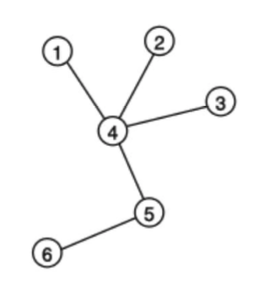
\includegraphics[width=100pt]{images/tree-graph.png}\hspace*{\fill}
  \caption{Example of Tree}
\end{figure}  \\
\textbf{Degree}: number of edges incident on a node \\
\textbf{Degree (directed graph)}: 
\begin{itemize}
	\item \uline{In degree}: number of edges entering the node
	\item \uline{Out degree}: number of edges leaving the node
	\item $Degree = indegree + outdegree$
\end{itemize}
\begin{figure}[h!]
\begin{minipage}{.5\textwidth}
  \centering
  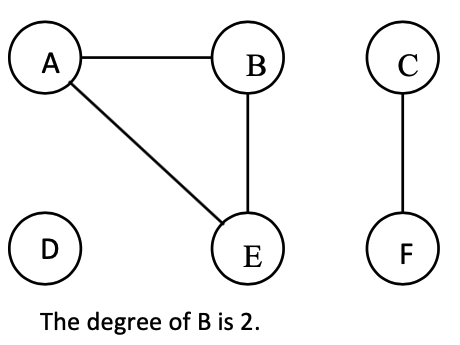
\includegraphics[width=.5\linewidth]{images/graph-degree}
  \captionof{figure}{Node degree}
\end{minipage}%
\begin{minipage}{.5\textwidth}
  \centering
  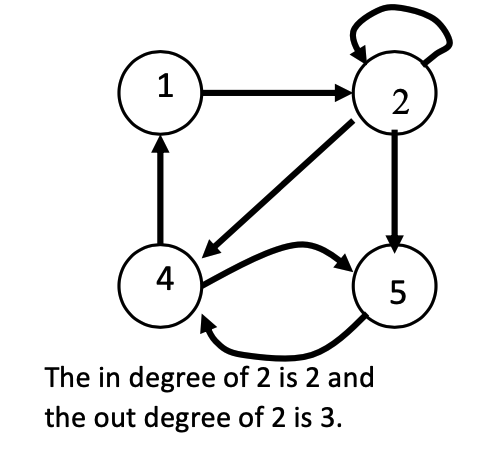
\includegraphics[width=.5\linewidth]{images/directed-graph-degree}
  \captionof{figure}{Node degree in directed graph}
\end{minipage}
\end{figure}
\textbf{Subgraph}: vertex and edge sets are subsets of those of G; a \uline{supergraph} of a graph G is a graph that contains G as a subgraph.
\begin{figure}[h!]
 \hfill 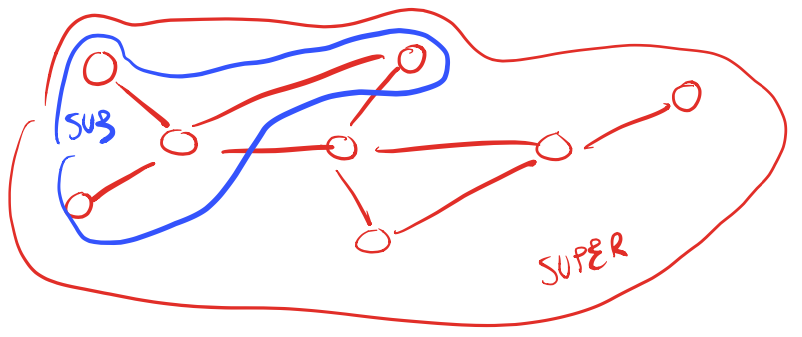
\includegraphics[width=150pt]{images/subgraph.png}\hspace*{\fill}
  \caption{Subgraph and Supergraph}
\end{figure} 
\pagebreak
\subsubsection{Graph Abstract Data Type (ADT)}
In computer science, a graph is an abstract data type (ADT) that consists of:
\begin{itemize}
	\item a set of nodes
	\item a set of edges (establish relationships/connections between the nodes)
\end{itemize}
The graph ADT follows directly from the graph concept from mathematics. We can implement a graph as a:
\begin{itemize}
	\item Matrix
	\begin{itemize}
		\item Incidence Matrix - [edge, vertex] contains the edge's data
		\item Adjacency Matrix - [vertex, vertex] boolean values (adjacent or not) or edge weights
	\end{itemize}
	\item List
	\begin{itemize}
		\item Edge List - pairs (ordered if directed) of vertices and optionally weight and other data
		\item Adjacency List
	\end{itemize}
\end{itemize}
\begin{figure}[h!]
 \hfill 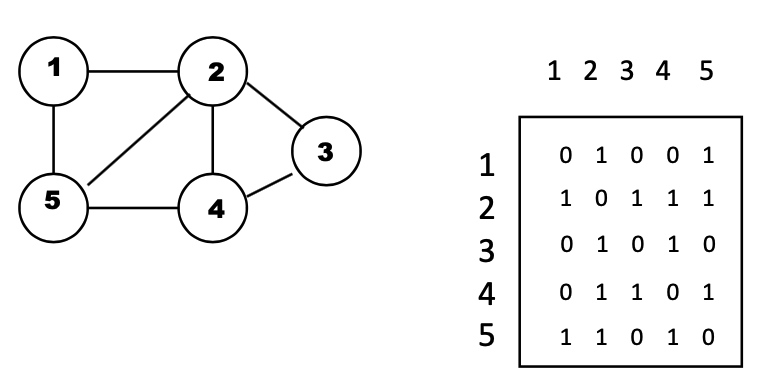
\includegraphics[width=100pt]{images/adjacency-matrix.png}\hspace*{\fill}
  \caption{$|V|x|V|$ matrix $A=(a_{ij})$ such that $a_{ij}=1$ if $(i,j) \in E$ and $0$ otherwise.}
\end{figure} 
\subsection{Graph Databases}
A \textbf{graph database management system} (henceforth, a graph database) is an online database management system with Create, Read, Update, and Delete (CRUD) methods that expose a graph data model. Graph databases are generally built for use with transactional (OLTP) systems. Accordingly, they are normally optimized for transac‐ tional performance, and engineered with transactional integrity and operational availability in mind. \nline
There are two properties of graph databases we should consider when investigating graph database technologies:
\begin{itemize}
	\item \textit{The underlying storage}: \\ Some graph databases use \uline{native graph storage} that is optimized and designed for storing and managing graphs. Not all graph database technologies use native graph storage, however. Some serialize the graph data into a relational database, an object-oriented database, or some other general-purpose data store.
	\item \textit{The processing engine}: \\ Some definitions require that a graph database use index-free adjacency, meaning that \uline{connected nodes physically “point” to each other in the database}. Here we take a slightly broader view: any database that from the user’s perspective behaves like a graph database (i.e., exposes a graph data model through CRUD operations) qualifies as a graph database. We do acknowledge, however, the significant performance advantages of index-free adjacency, and therefore use the term native graph processing to describe graph databases that leverage index-free adjacency.
\end{itemize}
\textcolor{blue}{\textit{It’s important to note that native graph storage and native graph processing are neither good nor bad $-$ they’re simply classic engineering trade-offs. The benefit of native graph storage is that its purpose-built stack is engineered for performance and scalability. The benefit of nonnative graph storage, in contrast, is that it typically depends on a mature nongraph backend (such as MySQL) whose production characteristics are well understood by operations teams. Native graph processing (index-free adjacency) benefits traversal performance, but at the expense of making some queries that don’t use traversals difficult or memory intensive.}} 
\nline
Relationships are first-class citizens of the graph data model. This is not the case in other database management systems, where we have to infer connections between entities using things like foreign keys or out-of-band processing such as map-reduce. By assembling the simple abstractions of nodes and relationships into connected structures, graph databases enable us to build arbitrarily sophisticated models that map closely to our problem domain. The resulting models are simpler and at the same time more expressive than those produced using traditional relational databases and the other NoSQL (Not Only SQL) stores.
\subsubsection{Advantages of Graph Databases}
\paragraph{Performance:}
One compelling reason, then, for choosing a graph database is the sheer \uline{performance increase when dealing with connected data versus relational databases and NoSQL stores}. In contrast to relational databases, where join-intensive query performance deteriorates as the dataset gets bigger, with a graph database performance tends to remain relatively constant, even as the dataset grows. This is because queries are localized to a portion of the graph. As a result, the execution time for each query is proportional only to the size of the part of the graph traversed to satisfy that query, rather than the size of the overall graph.
\paragraph{Flexibility:}
As developers and data architects, we want to connect data as the domain dictates, thereby allowing structure and schema to emerge in tandem with our growing understanding of the problem space, rather than being imposed upfront, when we know least about the real shape and intricacies of the data. Graph databases address this want directly. 
\nline
Graphs are naturally additive, meaning we can add new kinds of relationships, new nodes, new labels, and new subgraphs to an existing structure without disturbing existing queries and application functionality. These things have generally positive implications for developer productivity and project risk. Because of the graph model’s flexibility, we don’t have to model our domain in exhaustive detail ahead of time $-$ a practice that is all but foolhardy in the face of changing business requirements. The additive nature of graphs also means we tend to perform fewer migrations, thereby reducing maintenance overhead and risk.
\paragraph{Agility:} 
We want to be able to evolve our data model in step with the rest of our application, using a technology aligned with today’s incremental and iterative software delivery practices. Modern graph databases equip us to perform frictionless development and graceful systems maintenance. In particular, the schema-free nature of the graph data model, coupled with the testable nature of a graph database’s application programming interface (API) and query language, empower us to evolve an application in a controlled manner. 
\nline
At the same time, precisely because they are schema free, graph databases lack the kind of schema-oriented data governance mechanisms we’re familiar with in the relational world. But this is not a risk; rather, it calls forth a far more visible and actionable kind of governance. Governance is typically applied in a programmatic fashion, using tests to drive out the data model and queries, as well as assert the business rules that depend upon the graph.
\begin{figure}[h!]
\begin{minipage}{.5\textwidth}
  \centering
  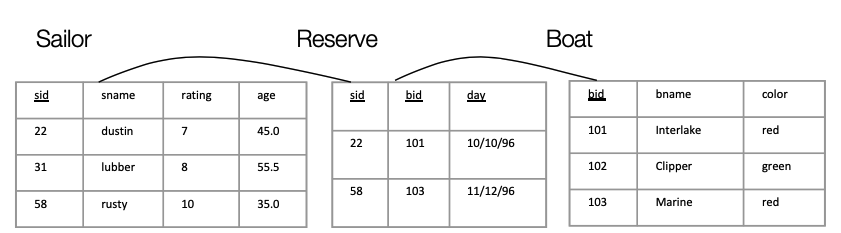
\includegraphics[width=.9\linewidth]{images/relational-db}
  \captionof{figure}{Relational DB with intermediate join table}
\end{minipage}%
\begin{minipage}{.5\textwidth}
  \centering
  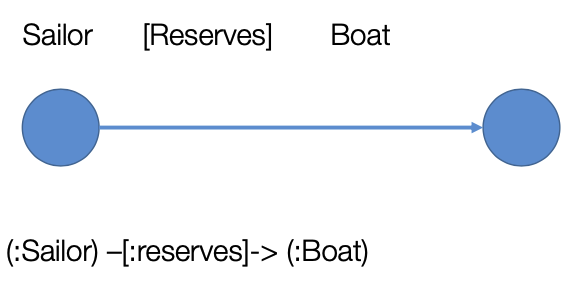
\includegraphics[width=.7\linewidth]{images/graph-db}
  \captionof{figure}{Graph DB model. Much simpler!}
\end{minipage}
\end{figure}
\begin{figure}[h!]
 \hfill 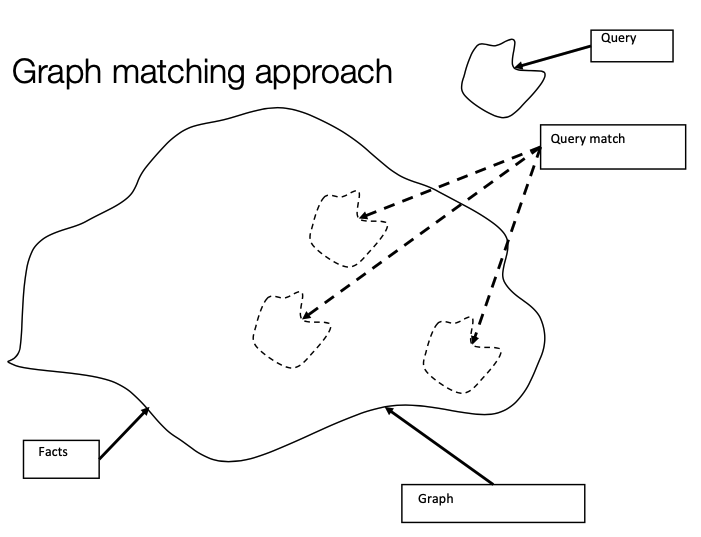
\includegraphics[width=150pt]{images/graph-query.png}\hspace*{\fill}
  \caption{Querying a graph is similar to pattern matching. First, we define a pattern (shape of (sub)graph that we are looking for) and then we look in the graph for that shape.}
\end{figure}  \\
\pagebreak
\subsection{Neo4J}
\textbf{Neo4J} is the most popular graph database, developed by Neo Technologies and implemented in Java. It is fully open source. \\
\uline{Salient features}
\begin{itemize}
	\item \textbf{Neo4J is schema free}: data does not have to adhere to any convention
	\item \textbf{ACID}: atomic, consistent, isolated and durable for logical units of work (fully transactional solution)
	\item Easy to get started and use
	\item Well documented and large developer community
	\item Support for wide variety of languages (Java, Python, Perl, Scala, Cypher, etc.)
\end{itemize}
\begin{figure}[h!]
 \hfill \includegraphics[width=180pt]{images/neo4j-arch.png}\hspace*{\fill}
  \caption{Neo4J software architecture. Each type of record (e.g., nodes, relationships) is stored in a separate and dedicated file. Traditional \textbf{C}onsistency and \textbf{Availability} support (no partitioning).}
\end{figure} 
Neo4J is meant to be an operational DB, not specifically for analytics. Thus, it is efficient on nodes and patterns, while is not so efficient in whole-graph analysis. \nline
The data model is composed by 
\begin{itemize}
	\item Nodes $-$ with labels (type) and attributes
	\item Edges
	\item Indexes (different from the ones in standard relational db) indexe
\end{itemize}
\subsubsection{Cypher}
Cypher is an expressive (yet compact) graph database query language. Cypher is arguably the easiest graph query language to learn, and is a great basis for learning about graphs. Cypher is designed to be easily read and understood by developers, database profes‐ sionals, and business stakeholders. Its ease of use derives from the fact that it is in accord with the way we intuitively describe graphs using diagrams. 
\nline
Cypher enables a user (or an application acting on behalf of a user) to ask the database to find data that matches a specific pattern. Colloquially, we ask the database to “find things like this.” And the way we describe what “things like this” look like is to draw them, using ASCII art.
\begin{figure}[h!]
 \hfill \includegraphics[width=150pt]{images/cypher-pattern.png}\hspace*{\fill}
  \caption{This pattern describes three mutual friends. Here’s the equivalent ASCII art representation in Cypher: \textcolor{blue}{(emil)$\leftarrow$[:KNOWS]$-$(jim)$-$[:KNOWS]$\rightarrow$(ian)$-$[:KNOWS]$\rightarrow$(emil)}
}
\end{figure}  \\
Cypher patterns follow very naturally from the way we draw graphs on the whiteboard.
\nline
The previous Cypher pattern describes a simple graph structure, but it doesn’t yet refer to any particular data in the database. To bind the pattern to specific nodes and relationships in an existing dataset we must specify some property values and node labels that help locate the relevant elements in the dataset. For example:

\begin{figure}[h!]
 \hfill \includegraphics[width=150pt]{images/cypher-pattern2.png}\hspace*{\fill}
  \caption{Here we have bound each node to its identifier using its $name$ property and $Person$ label. The $emil$ identifer, for example, is bound to a node in the dataset with a label $Person$ and a $name$ property whose value is $Emil$. Anchoring parts of the pattern to real data in this way is normal Cypher practice.}
\end{figure} 

Like most query languages, Cypher is composed of clauses. The simplest queries consist of a $MATCH$ clause followed by a $RETURN$ clause (we’ll describe the other clauses you can use in a Cypher query later in this chapter). Here’s an example of a Cypher query that uses these three clauses to find the mutual friends of a user named Jim:
\begin{figure}[h!]
 \hfill \includegraphics[width=250pt]{images/cypher-pattern3.png}\hspace*{\fill}
\end{figure}  \\
Other Cypher clauses:
\begin{itemize}
	\item \textbf{WHERE}: provides criteria for filtering pattern matching results.
	\item \textbf{CREATE} and \textbf{CREATE UNIQUE}: create nodes and relationships.
	\item \textbf{MERGE}: ensures that the supplied pattern exists in the graph, either by reusing existing nodes and relationships that match the supplied predicates, or by creating new nodes and relationships.
	\item \textbf{DELETE}: removes nodes, relationships, and properties.
	\item \textbf{SET}: sets property values.
	\item \textbf{FOREACH}: performs an updating action for each element in a list.
	\item \textbf{UNION}: merges results from two or more queries.
	\item \textbf{WITH}: chains subsequent query parts and forwards results from one to the next. Similar to piping commands in Unix.
	\item \textbf{START}: specifies one or more explicit starting points $-$ nodes or relationships $-$ in the graph. (START is deprecated in favor of specifying anchor points in a MATCH clause.)
\end{itemize}
\begin{figure}[h!]
 \hfill \includegraphics[width=150pt]{images/cypher-ex-query2.png}\hspace*{\fill}
 \caption{\textbf{Example query.} Find a node $n$ of type $Crew$ connected to $m$ with relations $r$ of type $Knows$ (from 1-step to *-steps in the relation) }
\end{figure}
\begin{figure}[h!]
 \hfill \includegraphics[width=150pt]{images/cypher-ex-query.png}\hspace*{\fill}
 \caption{\textbf{Example query.} Aggregation can be used (count). WITH separates query parts explicitly, to declare the variables for the next part. SKIP skips results at the top and LIMIT limits the number of results. }
\end{figure}
\begin{figure}[h!]
 \hfill \includegraphics[width=180pt]{images/cypher-ex-pattern1.png}\hspace*{\fill}
\end{figure}
\begin{figure}[h!]
 \hfill \includegraphics[width=250pt]{images/cypher-ex-pattern2.png}\hspace*{\fill}
   \caption{List of patterns}
\end{figure}
\paragraph{Stored procedures}
Cypher support stored procedures. It allows you to add JAVA functions or simply move a JAR to a folder to add new functions. Of course, there are also some predefined function such as \textit{shortestPath, allShortestPaths, size}.
\paragraph{Hints}
\begin{itemize}
	\item \textbf{Use parameters instead of literals} when possible. This allows Cypher to re-use your queries instead of having to parse and build new execution plans.
	\item \textbf{Always set an upper limit for your variable length patterns.} It’s easy to have a query touch all nodes in a graph by mistake.
	\item \textbf{Return only the data you need.} Avoid returning whole nodes and relationships
	\item Use \textbf{PROFILE / EXPLAIN} to analyze the performance of your queries.
\end{itemize}
\pagebreak
\section{Key-Value DB}
The main motivation behind Key-Value databases is performance. Indeed, there are certain organizations/companies that cannot accept low performances:
\begin{itemize}
	\item Amazon - Every 1/10 second delay resulted in 1\% loss of sales.
	\item Google - Half a second delay caused a 20\% drop in traffic
	\item Industrial Group - 1-second delay in page-load time
	\begin{itemize}
		\item 11\% fewer page views
		\item 15\% decrease in customer satisfaction
		\item 7\% loss in conversions
	\end{itemize}
\end{itemize}
Search by ID is usually built on top of a key-value store.
\begin{itemize}
	\item \uline{(Business) Key $\rightarrow$ Value} (follow this schema)
	\item (twitter.com) tweet $\rightarrow$ information about tweet
	\item (kayak.com) flight number $\rightarrow$ information about flight
	\item (yourbank.com) account number $\rightarrow$ information about it
	\item (amazon.com) item number $\rightarrow$ information about it
\end{itemize}
\subsection{How does a key-value database work?}
A key-value database, aka key-value store, associates a value (which can be anything from a number or simple string, to a complex object) with a key, which is used to keep track of the object. In its simplest form, a key-value store is like a dictionary/array/map object as it exists in most programming paradigms, but which is stored in a persistent way and managed by a Database Management System (DBMS). \nline
Key-value databases use compact, efficient index structures to be able to quickly and reliably locate a value by its key, making them ideal for systems that need to be able to find and retrieve data in constant time. Redis, for instance, is a key-value database that is optimized for tracking relatively simple data structures (primitive types, lists, heaps, and maps) in a persistent database. By only supporting a limited number of value types, Redis is able to expose an extremely simple interface to querying and manipulating them, and when configured optimally is capable of extremely high throughput. \nline
\subsubsection{Key Features}
A key-value database is defined by the fact that it allows programs or users of programs to retrieve data by keys, which are essentially names, or identifiers, that point to some stored value. Because key-value databases are defined so simply, but can be extended and optimized in numerous ways, there is no global list of features, but there are a few common ones:
\begin{itemize}
	\item \textbf{Retrieving a value} (if there is one) stored and associated with a given key
	\item \textbf{Deleting the value} (if there is one) stored and associated with a given key
	\item \textbf{Setting, updating, and replacing the value} (if there is one) associated with a given key
\end{itemize}

\subsection{Redis}
\textbf{RE}mote \textbf{DI}ctionary \textbf{S}erver (REDIS) introduced their key-value database in 2009. \nline
Redis is an advanced key-value store, where keys can contain data structures such as strings, hashes, lists, sets, and sorted sets. Supporting a set of atomic operations on these data types. \\
Redis is a different evolution path in the key-value databases where values are complex data types that are closely related to fundamental data structures and are exposed to the programmer as such, without additional abstraction layers. \\
It can be used as:
\begin{itemize}
	\item \textbf{Database} - Redis can persist data to disk
	\item \textbf{Caching layer} - Redis is fast
	\item \textbf{Message Broker} - Redis is not only a key-value store
\end{itemize}
What is \uline{NOT} Redis:
\begin{itemize}
	\item \textbf{Redis is not a replacement for Relational Databases} nor Document Stores.
	\item \textbf{It might be used complementary to a SQL relational store}, and/or NoSQL document store.
	\item Even when Redis offers configurable mechanisms for persistency, increased persistency will tend to increase latency and decrease throughput.
	\item \textbf{Best used for rapidly changing data} with a foreseeable database size (should fit mostly in memory).
\end{itemize}
Redis use cases:
\begin{itemize}
	\item Caching
	\item Counting things
	\item Blocking queues
	\item Pub/Sub (service bus)
	\item MVC Output Cache provider
	\item ASP.NET Session State provider
	\item Online user data (e.g., shopping cart, ...)
	\item ... any real-mine cross-platform, cross-application communication
\end{itemize}
\uline{When to consider Redis:}
\begin{itemize}
	\item \textbf{Speed is critical}
	\item More than just key-value pairs
	\item Dataset can fit in memory
	\item Dataset is not critical
\end{itemize}


\begin{figure}[ht!]
	\centering
	 \hfill \includegraphics[width=350pt]{images/redis-datatypes.png}\hspace*{\fill}
 \caption{Redis data types.}
 
 	\vspace{2em}
  \centering
  \hfill \includegraphics[width=250pt]{images/redis-commands1.png}\hspace*{\fill}

  \vspace{0.5em}

  \hfill \includegraphics[width=250pt]{images/redis-commands2.png}\hspace*{\fill}
 \caption{Redis commands. \href{https://redis.io/commands}{Full command reference here}}
\end{figure} 
\clearpage
\subsubsection{Scaling Redis}
\begin{itemize}
	\item \textbf{Persistence}: how can we be sure that we have some persistent storage of data (since Redis works in main memory)? \\ For this reason, REDIS provides two mechanisms to deal with persistence (very basic options):
	\begin{itemize}
		\item \uline{Redis Database Snapshots (RDB)}: save memory snapshot on disk (like a backup)
		\item \uline{append-only files (AOF)}: store in append mode the evolution of data
	\end{itemize}
	\item \textbf{Replication}: a Redis instance known as the \textit{master}, ensures that one or more instances known as the \textit{slaves}, become exact copies of the master. Clients can connect to the master or to the slaves. Slaves are read only by default, while master allows both read and write operations.
	\item \textbf{Partitioning}: we need to deal with data separation, breaking up data and distributing it across different hosts in a cluster. It can be implemented in different layers:
	\begin{itemize}
		\item \uline{Client}: partitioning on client-side code
		\item \uline{Proxy}: an extra layer that proxies all redis queries and performs partitioning \\ (i.e. \textcolor{blue}{Twemproxy})
		\item \uline{Query Router}: instances will make sure to forward the query to the right node\\  (i.e. \textcolor{blue}{Redis Cluster})
	\end{itemize}
	\item \textbf{Failover}: replace possible masters that are broken with a slave
	\begin{itemize}
		\item Manual
		\item Automatic with Redis Sentinel (for master-slave topology)
		\item Automatic with Redis Cluster (for cluster topology)
	\end{itemize}
\end{itemize}

\subsubsection{Redis topologies}

\begin{enumerate}
	\item Standalone
	\item Sentinel (automatic failover)
	\item Twemproxy (distribute data)
	\item Cluster (automatic failover and distribute data)
\end{enumerate}

\paragraph{I - Standalone} 
\begin{itemize}
	\item The master data is optionally replicated to slaves.
	\item The slaves provides data redundancy, reads offloading and save-to-disk offloading.
	\item Clients can connect to the Master for read/write operations or to the Slaves for read operations.
	\item Slaves can also replicate to its own slaves.
	\item There is no automatic failover.
\end{itemize}

\begin{figure}[h!]
 \hfill \includegraphics[width=270pt]{images/redis-standalone.png}\hspace*{\fill}
\end{figure} 

\paragraph{II - Sentinel} 
\begin{itemize}
	\item Redis Sentinel provides a reliable \textbf{automatic failover} in a master/slave topology, automatically promoting a slave to master if the existing master fails.
	\item Every deployment (master or slave) have a sentinel component that is able to check the status of the other servers. If the master goes down, a slave is selected to become a new master automatically.
	\item Sentinel does not distribute data across nodes.
\end{itemize}

\begin{figure}[h!]
 \hfill \includegraphics[width=180pt]{images/redis-sentinel.png}\hspace*{\fill}
\end{figure} 

\paragraph{III - Twemproxy} 
\begin{itemize}
	\item \href{https://github.com/twitter/twemproxy}{Twemproxy} (a project by twitter) works  as a proxy between the clients and many Redis instances.
	\item Is able to \textbf{automatically distribute data} among different standalone Redis instances.
	\item Supports consistent hashing with different strategies and hashing functions
	\item Multi-key commands and transactions are not supported.
\end{itemize}

\begin{figure}[h!]
 \hfill \includegraphics[width=350pt]{images/redis-twemproxy.png}\hspace*{\fill}
\end{figure} 

\paragraph{IV - Cluster} 
\begin{itemize}
	\item Redis Cluster \textbf{distributed data} across different Redis instances and \textbf{perform automatic failover} if any problem happens to any master instance.
	\item All nodes are directly connected with a service channel.
	\item The keyspace is divided into hash slots. Different nodes will hold a subset of hash slot.
	\item Multi-key commands are only allowed for keys in the same  hash slot.
\end{itemize}

\begin{figure}[h!]
 \hfill \includegraphics[width=180pt]{images/redis-cluster.png}\hspace*{\fill}
\end{figure} 

\subsubsection{Redis Advantages}
\begin{itemize}
	\item Performance
	\item Availability
	\item Fault-Tolerance
	\item Scalability (adaptability)
	\item Portability
\end{itemize}

\begin{figure}[h!]
 \hfill \includegraphics[width=300pt]{images/redis-performance.png}\hspace*{\fill}
 \caption{\href{https://redislabs.com/blog/the-proven-redis-performance/}{NoSQL \& SQL response performance comparison}. \\ Num of operations per unit of time - Average query time}
\end{figure} 

\subsection{Key-Value and Caching}
\subsubsection{What is Caching?}
From Wikipedia: \\ \textit{"A cache is a collection of data duplicating original values stored elsewhere or computed earlier, where the original data is expensive to fetch (owing to longer access time) or to compute, compared to the cost of reading the cache."} 
\nline

\textbf{Anatomy}:
\begin{itemize}
	\item Simple key/value storage
	\item Simple operations
	\begin{itemize}
		\item save
		\item get
		\item delete
	\end{itemize}
\end{itemize}
\pagebreak
\textbf{Terminology}:
\begin{itemize}
	\item Storage cost
	\item Retrieval cost (network load / algorithm load)
	\item Invalidation (keeping data up to data / removing irrelevant data)
	\item Replacement policy:
	\begin{itemize}
		\item FIFO - First in First Out
		\item LFU - Least Frequently Used (replace the cache entry used the least often in the recent past)
		\item LRU - Least Recently Used (replace the least recently used items first)
		\item MRU - Most Recently Used (replace, in contrast to LRU, the most recently used items first)
		\item Random vs. Belady's algorithm (predicting the information that will not be needed for the longest time in the future and replace it)
	\end{itemize}	 
	\item Cache concepts:
	\begin{itemize}
		\item Cold Cache: when the cache is empty or has irrelevant data, so that CPU needs to do a slower read from main memory for your program data requirement. 
		\item Warm Cache: when the cache contains relevant data, and all the reads for your program are satisfied from the cache itself.
	\end{itemize}
	\item Cache Hit and Cache Miss
	\begin{itemize}
		\item Hit: when an application needs data and finds that data in the cache (avoiding to look for it in main memory)
		\item Miss:  when an application needs data and doesn’t find it in the cache, so then it has to go and find the data on disc (takes more time).
	\end{itemize}
	\item Typical stats:
	\begin{itemize}
		\item $hit\_ratio = hits / (hits + misses)$
		\item $miss\_ratio = 1-hit\_ratio$
	\end{itemize}
\end{itemize}
\textbf{When to cache?}
\begin{itemize}
	\item Caches are only efficient when the benefits of faster access outweights the overhead of checking and keeping your cache up to data
	\item More cache hits than cache misses
\end{itemize}
\textbf{Where are caches users?}
\begin{itemize}
	\item At hardware level (CPU, HDD)
	\item Operating systems (RAM)
	\item Web stack (browser cache, DNS cache, CDNs cache, application level)
	\item Applications
\end{itemize}
\pagebreak
\subsubsection{Memcached}
\begin{itemize}
	\item Free \& open-source, high-performance, distributed memory object caching system
	\item Generic in nature, intended for use in speeding up dynamic web applications by alleviating database load.
	\item Key/Value dictionary
	\item Now used by Netlog, Facebook, Flickr, Wikipedia, Twitter, Youtube ...
\end{itemize}
Technically, Memcached is a server, where client access over TCP or UDP. Servers can run in pools and are independent, clients manage the pool (e.g., 3 servers with 64GB mem each give you a single pool of 192GB storage for caching). \\
What to store in a memcache?
\begin{itemize}
	\item High demand (data used often)
	\item Expensive (data hard to compute)
	\item Common (data shared across users)
	\item typical examples:
	\begin{itemize}
		\item user sessions (often)
		\item user data (often, shared)
		\item homepage data (often, shared, expensive)
	\end{itemize}
\end{itemize}
\textbf{Memcached principles}
\begin{itemize}
	\item \textcolor{blue}{Very simple version of a data store}
	\item \textcolor{blue}{Lightweight technology with high-performance} (\textcolor{red}{comes at a cost})
 	\item \textcolor{blue}{Fast network access}: memcached servers close to other application servers
	\item \textcolor{red}{No persistency}: if your server goes down, data in memcached is gone
	\item \textcolor{red}{No redundancy / fail-over}
	\item \textcolor{red}{No replication}: single item in cache lives on one server only
	\item \textcolor{red}{No authentication}: not used in shared environments
	\item 1 key is maximum 1MB
	\item Keys are string of 250 characters
	\item No enumeration of keys: thus no list of valid keys in cache at certain moment)
	\item No active clean-up (only clean up when more space needed, LRU policy)
\end{itemize}
\begin{figure}[h!]
\centering
\begin{minipage}{.5\textwidth}
  \centering
  \includegraphics[width=.8\linewidth]{images/memcached-php}
  \captionof{figure}{Memcached PHP Client functions.}
\end{minipage}%
\begin{minipage}{.5\textwidth}
  \centering
  \includegraphics[width=.8\linewidth]{images/memcached-example}
  \captionof{figure}{Code for explicitly implementing caching.}
\end{minipage}
\end{figure}
\pagebreak
\section{Big Column DB}
\subsection{Introduction}
\subsubsection{Column wise vs. Row wise database}
A \textbf{columnar database stores data by columns} rather than by rows, which makes it suitable for analytical query processing, and thus for data warehouses. They're often used in data warehouses, the structured data repositories that businesses use to support corporate decision-making. \\
The major difference in both the datastores (row- vs column-based lies in the way they physically store the data on the disk. We know that persistent storage disks (hard disks) are organized in blocks and have following usual properties for reading/write operations. Head Seek operation is expensive in disks due to mechanical movement required. Read/Write is quite fast.
\begin{enumerate}
	\item The whole block with data is loaded into the memory for reading by the operating system. Any further read for data for this block will happen from memory and will be super fast.
	\item Read/Writing operations on disks are not slow. Only the seek operation is slow. i.e. to move the head to the correct block to perform the operation.
	\item Due to the above point — sequential read/writes are much faster on disks rather than the random access.
\end{enumerate}
Here comes the main difference between row and columnar DBs. \\
\textbf{Row oriented database tries to store whole row of the database in the same block but columnar database stores the values of the columns of subsequent in the same block} 
\nline
Indeed, columnar storage for database tables is an important factor in optimizing analytic query performance because it drastically reduces the overall disk I\/O requirements and reduces the amount of data you need to load from disk.
\nline
The following series of illustrations (from \href{https://docs.aws.amazon.com/redshift/latest/dg/c_columnar_storage_disk_mem_mgmnt.html}{Amazon Redshift documentation}) describe how columnar data storage implements efficiencies and how that translates into efficiencies when retrieving data into memory.
\begin{figure}[h!]
 \hfill \includegraphics[width=240pt]{images/columnar-vs-row1.png}\hspace*{\fill}
 \caption{Row-wise}
\end{figure}  \\
In a typical relational database table, each row contains field values for a single record. In row-wise database storage, data blocks store values sequentially for each consecutive column making up the entire row. In online transaction processing (OLTP) applications, most transactions involve frequently reading and writing all of the values for entire records, typically one record or a small number of records at a time. As a result, row-wise storage is optimal for OLTP databases.
\begin{figure}[h!]
 \hfill \includegraphics[width=240pt]{images/columnar-vs-row2.png}\hspace*{\fill}
 \caption{Column-wise}
\end{figure}  \\
Using columnar storage, each data block stores values of a single column for multiple rows. This means that reading the same number of column field values for the same number of records requires a third of the I/O operations compared to row-wise storage. In practice, using tables with very large numbers of columns and very large row counts, storage efficiency is even greater. An added advantage is that, since each block holds the same type of data, block data can use a compression scheme selected specifically for the column data type, further reducing disk space and I/O.
\nline
\subsubsection{Column storage}
\paragraph{Issues with today's workloads}
Column data storage were born to address the need of large scale data analysis.
\begin{itemize}
	\item Data large and unstructured
	\item Lots of random reads and writes
	\item Foreign keys rarely needed (we use more complex data structured)
	\item Actual needs:
	\begin{itemize}
		\item Incremental scalability
		\item Speed
		\item No single point of failure
		\item Low cost (TCO) and admin
		\item Scale out, not up
	\end{itemize}
\end{itemize}
Recalling the CAP Theorem, for which we can achieve at most 2 out of the 3 guarantees (Consistency, Availability and Partition-tolerance), usually column databases (e.g., Cassandra) focus on Availability and Partition-tolerance, supporting only Eventual (weak) Consistency. Indeed, they are mainly used in OLAP systems (online analytical processing) and data mining operations.
\begin{figure}[h!]
 \hfill \includegraphics[width=250pt]{images/column-vs-row.png}\hspace*{\fill}
 \caption{Column vs. Row data storage}
\end{figure} \\
\textcolor{blue}{\textbf{Pros}}:
\begin{itemize}
	\item Data compression (1000 TB compression come handy)
	\item Improved Bandwidth Utilization
	\item Improved Code Pipelining
	\item Improved Cache Locality
\end{itemize}
\textcolor{red}{\textbf{Cons}}
\begin{itemize}
	\item Increased Disk Seek Time
	\item Increased cost of Inserts
	\item Increased tuple reconstruction costs
\end{itemize}
\begin{figure}[h!]
\centering
\begin{minipage}{.5\textwidth}
  \centering
  \includegraphics[width=.7\linewidth]{images/tuple-reconstruction1}
  \captionof{figure}{Row based always read the entire row (constant time). Column based instead are more efficient when few bytes have to be read. Then there is a breakeven point after which row based databases become more efficient to read data.}
\end{minipage}%
\begin{minipage}{.5\textwidth}
  \centering
  \includegraphics[width=.7\linewidth]{images/tuple-reconstruction2}
  \captionof{figure}{Tuple reconstruction.}
\end{minipage}
\end{figure}
\paragraph{Compression}
Compression: find a better encoding without losing information
\begin{itemize}
	\item Trades I/O for CPU
	\item Increased column-store opportunities:
	\begin{itemize}
		\item Higher data value locality (spatial and temporal) in column stores, saving space and performance
		\item Techniques such as \textit{run length encoding} is far more useful
		\item Can use extra space to store multiple copies of data in different sort orders
	\end{itemize}
\end{itemize}
Example:
\begin{figure}[h!]
 \hfill \includegraphics[width=300pt]{images/column-compression-ex.png}\hspace*{\fill}
 \caption{Column compression example using Run Length encoding}
\end{figure} 
\pagebreak
\subsection{Cassandra}
Cassandra is a columnar database which was originally designed at Facebook and then open-sourced (now within Apache foundation. Many big companies use Cassandra: IBM, eBay, twitter, Adobe, Netflix, Spotify ...
\\
Cassandra can be considered an hybrid of Google's Bigtable (columnar) and Amazon's Dynamo (key-value). By the way it emphasizes a lot on columnar features.
\begin{figure}[h!]
 \hfill \includegraphics[width=350pt]{images/cassandra-data-model.png}\hspace*{\fill}
 \caption{Cassandra Data Model}
\end{figure}
\begin{figure}[h!]
 \hfill \includegraphics[width=350pt]{images/cassandra-vs-rdbms.png}\hspace*{\fill} \center
  \hfill \includegraphics[width=350pt]{images/cassandra-vs-rdbms2.png}\hspace*{\fill}
 \caption{Cassandra properties w.r.t. RDBMS (e.g., Oracle)}
\end{figure} \\
\raggedright
\pagebreak
\subsubsection{Cassandra Properties}
\begin{itemize}
	\item \textbf{highly available}
	\item \textbf{fault tolerant}
	\item \textbf{}\textit{tuneably} consistent: allows to have some levels of consistency which can be tuned dynamically (trade-off with performance)
	\item very fast writes
	\item linear, elastic scalability
	\item \textbf{decentralized/symmetric} (no master/slave)
	\item automatic provisioning of new nodes
	\item $O(1)$ DHT: key-based query $\rightarrow$  \uline{constant complexity}
\end{itemize}

\subsubsection{Gossip Protocol}
How does the Cassandra Cluster know which members are online and working? \\ It uses a \href{https://docs.datastax.com/en/cassandra-oss/3.0/cassandra/architecture/archGossipAbout.html}{gossip protocol}. \nline 
\textit{Gossip} is a peer-to-peer communication protocol in which nodes periodically exchange state information about themselves and about other nodes they know about. The gossip process runs every second and exchanges state messages with up to three other nodes in the cluster. The nodes exchange information about themselves and about the other nodes that they have gossiped about, so all nodes quickly learn about all other nodes in the cluster.
\begin{figure}[h!]
 \hfill \includegraphics[width=240pt]{images/gossip-protocol.png}\hspace*{\fill}
 \caption{Cassandra Gossip Protocol}
\end{figure}

\subsubsection{Replica Placement Strategies}
As hardware problem can occur or link can be down at any time during data process, a solution is required to provide a backup when the problem has occurred. So data is replicated for assuring no single point of failure. \nline
Cassandra places replicas of data on different nodes based on these two factors.
\begin{itemize}
	\item Where to place next replica is determined by the \textbf{Replication Strategy}.
	\item While the total number of replicas placed on different nodes is determined by the \textbf{Replication Factor}.
\end{itemize}
One Replication factor means that there is only a single copy of data while three replication factor means that there are three copies of the data on three different nodes. For ensuring there is no single point of failure, \textbf{replication factor must be three.} \pagebreak \\
There are two kinds of replication strategies in Cassandra.
\begin{itemize}
	\item \textbf{Simple Strategy}: used when you have just one data center. SimpleStrategy places the first replica on the node selected by the partitioner. After that, remaining replicas are placed in clockwise direction in the Node ring. 
	\begin{figure}[h!]
 \hfill \includegraphics[width=250pt]{images/cassandra-simple-strategy.png}\hspace*{\fill}
 \caption{Cassandra's topology can be imagined as a ring, in which nodes are all equivalent (master-less). The process of replication is managed by a coordinator (who changes each time), who's in charge of handling the a write operation and then start propagating the new value to the others. The replicas in turn, will continue propagating the new value in an asynchronous way, following the clockwise direction.}
\end{figure}
	\item \textbf{Network Topology Strategy}: is used when you have more than two data centers. In NetworkTopologyStrategy, replicas are set for each data center separately. NetworkTopologyStrategy places replicas in the clockwise direction in the ring until reaches the first node in another rack. This strategy tries to place replicas on different racks in the same data center. This is due to the reason that sometimes failure or problem can occur in the rack. Then replicas on other nodes can provide data.

\begin{figure}[h!]
 \hfill \includegraphics[width=250pt]{images/network-topology-strategy.png}\hspace*{\fill}
\end{figure}
\end{itemize}
\subsubsection{Write operation}
For performance reasons, write operations need to be lock-free and fast (no reads or disk seeks.\\ 
A Client sends a write to one front-end node in Cassandra cluster (coordinator). The coordinator forwards the request to replicas that are responsible for that key. 
\begin{itemize}
	\item Always writable: \uline{Hinted Handoff} 
	\begin{itemize}
		\item If any replica is down, the coordinator writes to all other replicas, and keeps the write until down replica comes back up.
		\item When all replicas are down, the Coordinator buffers writes (up to an hour).
	\end{itemize}	
	\item Provides \uline{Atomicity} for a given key (i.e., within ColumnFamily)
\end{itemize}
\textbf{Consistency level} determines how many nodes will respond back with the success acknowledgment. The node will respond back with the success acknowledgment if data is written successfully to the commit log and \textbf{mem-table}. \nline
For example, in a single data center with replication factor equals to three, three replicas will receive write request. If consistency level is one, only one replica will respond back with the success acknowledgment, and the remaining two will remain dormant. Suppose if remaining two replicas lose data due to node downs or some other problem, Cassandra will make the row consistent by the built-in repair mechanism in Cassandra. \nline

Here it is explained, how write process occurs in Cassandra:
\begin{enumerate}
	\item When write request comes to the node, first of all, it logs in the commit log.
	\item Then Cassandra writes the data in the mem-table. Data written in the mem-table on each write request also writes in commit log separately. Mem-table is a temporarily stored data in the memory while Commit log logs the transaction records for back up purposes.
	\item When mem-table is full or old, data is flushed to the SSTable data file.
\end{enumerate}
\subsubsection{Read operation}
Are we sure that copies in replicas are aligned? That's why read operations may be slower than writes because they need to touch log and multiple SSTables to check if the data is correct. \nline
There are three types of read requests that a coordinator sends to replicas.
\begin{itemize}
	\item Direct request
	\item Digest request
	\item Read repair request
\end{itemize}
The coordinator sends direct request to one of the replicas. After that, the coordinator sends the digest request to the number of replicas specified by the consistency level and checks whether the returned data is an updated data.
\nline
After that, the coordinator sends digest request to all the remaining replicas. If any node gives out of date value, a background read repair request will update that data. This process is called read repair mechanism.
\subsubsection{Cassandra Quorums and Consistency Levels}
What if we have different values for the same data? Play with \textbf{majority quorums}. \\
Cassandra’s tunable consistency comes from the fact that it allows per-operation tradeoff between consistency and availability through consistency levels.  \\
The following consistency levels are available:
\begin{itemize}
	\item $ONE$ – Only a single replica must respond.
	\item $TWO$ – Two replicas must respond.
	\item $THREE$ – Three replicas must respond.
	\item $QUORUM$ – A majority (n/2 + 1) of the replicas must respond.
	\item $ALL$ – All of the replicas must respond.
	\item $LOCAL\_QUORUM$ – A majority of the replicas in the local datacenter (whichever datacenter the coordinator is in) must respond.
	\item $EACH\_QUORUM$ – A majority of the replicas in each datacenter must respond.
	\item $ANY$ – A single replica may respond, or the coordinator may store a hint. If a hint is stored, the coordinator will later attempt to replay the hint and deliver the mutation to the replicas. This consistency level is only accepted for write operations.
\end{itemize}
\begin{figure}[ht!]
 \hfill \includegraphics[width=250pt]{images/cassandra-write-consistency.png}\hspace*{\fill}
 \caption{Cassandra write consistency}
\end{figure}
\begin{figure}[ht!]
 \hfill \includegraphics[width=250pt]{images/cassandra-read-consistency.png}\hspace*{\fill}
  \caption{Cassandra read consistency}
\end{figure} 
\pagebreak
\subsubsection{Data model}
\begin{figure}[ht!]
 \hfill \includegraphics[width=200pt]{images/cassandra-data-model2.png}\hspace*{\fill}
  \caption{Cassandra data model}
\end{figure} 
 The \textbf{keyspace} is the entire DB, the space in which we define the keys for the elements and typically there is one keyspace per applications. Each \textbf{column} consists of a name (key), a value and a clock timestamp which indicates the update time. Furthermore every column is part of a \textbf{column family}. Indeed, a column family is a group of records of \textit{similar} kind of elements (not the \textit{same} kind, because CFs are \textcolor{red}{sparse tables}). Some examples of column families are: User, Address, Tweet, PointOfInterest, HotelRoom.
 
 \begin{figure}[ht!]
 \hfill \includegraphics[width=200pt]{images/cassandra-column-family.jpg}\hspace*{\fill}
  \caption{Cassandra column families are sparse tables. Some rows may contain all columns, while in other rows there could be only some of them. As in this case, row 104 has only one column while row 103 has 4 columns.}
\end{figure} 

\pagebreak
\begin{figure}[ht!]
 \hfill \includegraphics[width=250pt]{images/cassandra-data-model3.png}\hspace*{\fill}
  \caption{Cassandra: hybrid key-value based + column based database.}
\end{figure} 
Cassandra, as we mentioned earlier, is an hybrid hybrid key-value based and column based database. Indeed, we can see that each row has a key and is composed by a set of columns (the value). Somehow we could say that Cassandra is a key-value based database in which the value is internally structured as columns.

\begin{figure}[ht!]
 \hfill \includegraphics[width=250pt]{images/cassandra-supercolumn.png}\hspace*{\fill}
  \caption{Cassandra supercolumn}
\end{figure} 
In Cassandra there's also the concept of \textbf{super column}. Super columns group columns under a common name.

\begin{figure}[h!]
\centering
\begin{minipage}{.5\textwidth}
  \centering
  \includegraphics[width=.8\linewidth]{images/cassandra-super-column-family}
\end{minipage}%
\begin{minipage}{.5\textwidth}
  \centering
  \includegraphics[width=.8\linewidth]{images/cassandra-super-column-family2}
\end{minipage}
\caption{Supercolumn families}
\end{figure}

\subsubsection{What about...SQL?}
\begin{itemize}
	\item \textbf{RDBMS}: domain-based-model $\rightarrow$ \textit{what answers do I have?} (schema on write)
	\begin{enumerate}
		\item Create the schema
		\item Perform query
		\item Check answer/result
	\end{enumerate}
	\item \textbf{Cassandra}: \textcolor{red}{query-based model} $\rightarrow$ \textit{what \uline{questions} do I have?} (schema on read)
	\begin{enumerate}
		\item Plan the query
		\item Create the schema
		\item Check answer/result
	\end{enumerate}
\end{itemize}
\pagebreak
In Cassandra we start defining queries and then we design the data model. Indeed, we define Cassandra as an \textit{index factory}.

\begin{figure}[ht!]
 \hfill \includegraphics[width=150pt]{images/cassandra-index.png}\hspace*{\fill}
  \caption{Given the schema defined above, how could we support the presented query? We just create a new column family $UserCity$ which supports our query. In this case we are querying on the city attribute, that's why the new column family contains all the IDs of the users in that city.}
\end{figure}
 
\begin{figure}[ht!]
\centering
\begin{minipage}{.5\textwidth}
  \centering
  \includegraphics[width=.8\linewidth]{images/rdbms-schema}
\end{minipage}%
\begin{minipage}{.5\textwidth}
  \centering
  \includegraphics[width=.8\linewidth]{images/cassandra-schema}
\end{minipage}
\caption{RDBMS schema are rigid schema defined when building up the database. Cassandra schema is more flexible because new column families are continuously added according to query needs. }
\end{figure} 
 
 \subsection{Is Cassandra a good fit?}
 Cassandra is a good fit when:
 \begin{itemize}
 	\item you need really fast writes
 	\item you need durability
 	\item you have lots of data
	\begin{itemize}
		\item $> GBs$ (e.g., billions of tweets)
		\item more than three servers)
	\end{itemize} 	
	\item your app is evolving (startup mode, fluid data structure)
	\item loose domain data ("point of interest")
	\item your programmers can deal with
	\begin{itemize}
		\item documentation
		\item complexity
		\item consistency model
		\item change
		\item visibility tools
	\end{itemize}
 \end{itemize}
 \paragraph{Vs. SQL}
  With more than 50GB of data:
 \begin{itemize}
 	\item MySQL
 	\begin{itemize}
 		\item Writes 300ms avg
 		\item Reads 350ms avg
 	\end{itemize}
 	\item Cassandra
 	\begin{itemize}
 		\item Writes 0.12ms avg
 		\item Reads 15ms avg
 	\end{itemize}
 \end{itemize}
 \pagebreak
 \section{Document-oriented DB}
 \subsection{Why document-based?}
 What makes document databases different from relational databases?
 
 \begin{enumerate}
 	\item \textbf{Intuitive Data Model}: Faster and Easier for Developers \\
 	Documents map to the objects in your code, so they are much more natural to work with. There is no need to decompose data across tables, run expensive JOINs, or integrate a separate ORM layer. Data that is accessed together is stored together, so you have less code to write and your users get higher performance.
 	\item \textbf{Flexible Schema}: Dynamically Adapt to Change \\
 	A document’s schema is dynamic and self-describing, so you don’t need to first pre-define it in the database. Fields can vary from document to document and you modify the structure at any time, avoiding disruptive schema migrations. Some document databases offer JSON Schema so you can optionally enforce rules governing document structures.
 	\item \textbf{Universal}: JSON Documents are Everywhere \\
 	Lightweight, language-independent, and human readable, JSON has become an established standard for data interchange and storage. Documents are a superset of all other data models so you can structure data any way your application needs – rich objects, key-value pairs, tables, geospatial and time-series data, and the nodes and edges of a graph. You can work with documents using a single query language, giving you a consistent development experience however you’ve chosen to model your data.
 	\item \textbf{Powerful}: Query Data Anyway You Need \\
 	An important difference between document databases is the expressivity of the query language and richness of indexing. The MongoDB Query Language is comprehensive and expressive. Ad hoc queries, indexing, and real time aggregations provide powerful ways to access, transform, and analyze your data. With ACID transactions you maintain the same guarantees you’re used to in SQL databases, whether manipulating data in a single document, or across multiple documents living in multiple shards.
 	\item \textbf{Distributed}: Resilient and Globally Scalable \\ 
 	Unlike monolithic, scale-up relational databases, document databases are distributed systems at their core. Documents are independent units which makes it easier to distribute them across multiple servers while preserving data locality. Replication with self-healing recovery keeps your applications highly available while giving you the ability to isolate different workloads from one another in a single cluster. Native sharding provides elastic and application-transparent horizontal scale-out to accommodate your workload’s growth, along with geographic data distribution for data sovereignty.
 \end{enumerate}
 
 \begin{figure}[ht!]
 \hfill \includegraphics[width=250pt]{images/document-based.png}\hspace*{\fill}
  \caption{Example of document (invoice) stored in a document-based database.}
\end{figure}  

The document in Figure 71 is made of nested data object which (hypothetically) corresponds to different database tables. We decide to use document-based databases if we usually want to retrieve the data in an aggregate way, avoiding complex joins between table. Indeed, we query the database and we obtain a document with all its subdocuments included. \nline
 
\begin{figure}[ht!]
 \hfill \includegraphics[width=300pt]{images/relational-to-document.png}\hspace*{\fill}
  \caption{Example of JSON document}
\end{figure}  
 
\subsection{MongoDB}

\begin{itemize}
	\item An open source and document-oriented database
	\item Data is stored in JSON-like documents
	\item Designed with both scalability and developer agility
	\item Dynamic schemas
	\item Automatic data sharding
\end{itemize} 
 
\begin{figure}[ht!]
 \hfill \includegraphics[width=300pt]{images/mongodb-features.png}\hspace*{\fill}
  \caption{MongoDB features.}
  \end{figure}
  
\begin{figure}[ht!]
 \hfill \includegraphics[width=250pt]{images/mongodb-vs-sql.png}\hspace*{\fill}
  \caption{MongoDB terminology vs SQL.}
\end{figure}  
  
\subsubsection{Facts}
\begin{itemize}
	\item No schemas
	\item No transactions
	\item No joins
	\item Max document size of 16MB (larger documents are handled with GridFS)
	\item Runs on most common OSs (Windows, Linux, Mac)
	\item Data stored as BSON (Binary JSON)
	\begin{itemize}
		\item used for speed
		\item translation handled by language drivers
	\end{itemize}
\end{itemize}
 
\subsubsection{Data Model} 

\begin{figure}[ht!]
\centering
\begin{minipage}{.5\textwidth}
  \centering
  \includegraphics[width=.8\linewidth]{images/mongodb-data-model}
    \caption{A collection includes a set of documents.}
\end{minipage}%
\begin{minipage}{.5\textwidth}
  \centering
  \includegraphics[width=.8\linewidth]{images/mongodb-data-model2}
  \caption{Structure of a JSON-document. The value of field could be one of: native data types, arrays, other documents. \uline{Rule: every document must have an \_id.}}
\end{minipage}
\end{figure} 

\begin{figure}[ht!]
\centering
\begin{minipage}{.5\textwidth}
  \centering
  \includegraphics[width=.8\linewidth]{images/mongodb-embedded}
    \caption{Embdedded documents.}
\end{minipage}%
\begin{minipage}{.5\textwidth}
  \centering
  \includegraphics[width=.8\linewidth]{images/mongodb-reference}
  \caption{Reference documents or linking documents.}
\end{minipage}
\end{figure} 
\subsubsection{Queries}

\begin{figure}[ht!]
\centering
\begin{minipage}{.5\textwidth}
  \centering
  \includegraphics[width=.8\linewidth]{images/mongodb-read-mapping}
    \caption{Read queries compared to SQL.}
\end{minipage}%
\begin{minipage}{.5\textwidth}
  \centering
  \includegraphics[width=.8\linewidth]{images/mongodb-comparison-op}
  \caption{Comparison operators.}
\end{minipage}
\end{figure} 
 
 \subsubsection{CAP Theorem and Mongo}
 Relative to the CAP theorem, MongoDB is a \textbf{CP} data store—it resolves network partitions by maintaining consistency, while compromising on availability.
 \nline
 MongoDB is a single-master system—each replica set can have only one primary node that receives all the write operations. All other nodes in the same replica set are secondary nodes that replicate the primary node's operation log and apply it to their own data set. By default, clients also read from the primary node, but they can also specify a read preference that allows them to read from secondary nodes.
 \nline
 When the primary node becomes unavailable, the secondary node with the most recent operation log will be elected as the new primary node. Once all the other secondary nodes catch up with the new master, the cluster becomes available again. As clients can't make any write requests during this interval, the data remains consistent across the entire network.
 \pagebreak
\section{Streaming Data Engineering}
 
 \begin{figure}[ht!]
\centering
\begin{minipage}{.5\textwidth}
  \centering
  \includegraphics[width=.9\linewidth]{images/big-data-logical-arch}
\end{minipage}%
\begin{minipage}{.5\textwidth}
  \centering
  \includegraphics[width=.9\linewidth]{images/big-data-logical-arch2}
\end{minipage}
\caption{Logical architecture of a Big Data Platform.}
\end{figure} 

Big data architecture is the foundation for big data analytics. It is the overarching system used to manage large amounts of data so that it can be analyzed for business purposes, steer data analytics, and provide an environment in which big data analytics tools can extract vital business information from otherwise ambiguous data. The big data architecture framework serves as a reference blueprint for big data infrastructures and solutions, \textbf{logically defining how big data solutions will work, the components that will be used, how information will flow, and security details.}


\subsection{The Solution Space}
\subsubsection{The Dimensions: Throughput vs. Latency vs. Message size}

\begin{figure}[ht!]
 \hfill \includegraphics[width=220pt]{images/the-dimensions.png}\hspace*{\fill}
\end{figure}  
In Figure 82, trucks are transporting data (they can carry a certain amount of data). Data can be ingested in our system at a certain speed, expecting different latency according to the size to be ingested.  \\
\textbf{Throughput} indicates how much data we are able to ingest in a given time interval. It is the main performance indicator that we aim to optimize. \\
We have three options to optimize throughput:
\begin{itemize}
	\item Increase trucks' speed
	\item Add lanes to the streets (parallelize)
	\item Reduce trucks' size (compress data)
\end{itemize}
\begin{figure}[ht!]
 \hfill \includegraphics[width=180pt]{images/increase-throughput.png}\hspace*{\fill}
\end{figure}  
\begin{figure}[ht!]
 \hfill \includegraphics[width=170pt]{images/latency-throughput.png}\hspace*{\fill}
 \caption{Latency-Throughput trade-off}
\end{figure}  

\pagebreak
\subsubsection{Three Cases along a continuum}

 \begin{figure}[ht!]
\centering
\begin{minipage}{.5\textwidth}
  \centering
  \includegraphics[width=.8\linewidth]{images/three-cases-continuum}
\end{minipage}%
\begin{minipage}{.5\textwidth}
  \centering
  \includegraphics[width=.8\linewidth]{images/three-cases}
\end{minipage}
\caption{Three cases and their latency-throughput trade-off.}
\end{figure} 

\paragraph{Ultra Bulk Case:} \textcolor{red}{high throughput and high latency} \\
Transfer Appliance is a secure, rackable high capacity storage server that you set up in your datacenter. You fill it with data and ship it to an ingest location where the data is uploaded to Google Cloud Storage. Your data is encrypted automatically, and remains safe until you decrypt it.

 \begin{figure}[ht!]
\centering
\begin{minipage}{.5\textwidth}
  \centering
  \includegraphics[width=.6\linewidth]{images/ultra-bulk}
\end{minipage}%
\begin{minipage}{.5\textwidth}
  \centering
  \includegraphics[width=.6\linewidth]{images/google-cloud-transfer}
\end{minipage}
\caption{With \href{https://cloud.google.com/transfer-appliance/}{Google Cloud Transfer Appliance}, you need only 2 days to upload 1PB to cloud.}
\end{figure}

\paragraph{Continuous Case} \textcolor{red}{low throughput and low latency} \nline
Example: Real Time Inventory \\
A company has 10k shops distributed all over the planet and an e-commerce site divided in 5/7 areas, with a total of 100k distinct products. To optimize the shipping time they further transform each shop in a shipping point for their products, thus we now have 10k micro market area for the e-commerce (one per each shop). They receive around 10k purchase/s and each message has a size of 100KB. The required throughput for the system is 200MB/s, which is easy to achieve with a Kafka cluster with 10 nodes.
\begin{figure}[ht!]
 \hfill \includegraphics[width=270pt]{images/continuous.png}\hspace*{\fill}
\end{figure}  

\paragraph{Batch Case} \textcolor{red}{balanced throughput-latency trade-off} \nline

Example: customer 360° journey \\
Here a customer accessing to an e-commerce is sending request to three different subsystems which are handling the different section of the size. Each modification performed on one of the subsystems is captured and stored in a blob storage service and then asynchronously propagated to a data warehouse for analytics purposes. The latency of the process can vary from minutes to days.
\begin{figure}[ht!]
 \hfill \includegraphics[width=350pt]{images/batch-case.png}\hspace*{\fill}
\end{figure}  
\subsection{The Batch Case}
In a distributed system dealing with Big Data (where complex failure patterns can happen) we usually apply \textbf{Write Once, Read Many principles}
\begin{itemize}
	\item allows reliable and parallel writing
	\item simplifies data coherency issues
	\item enables high throughput data access.
\end{itemize}
As a consequence:
\begin{itemize}
	\item All data are kept in \textbf{immutable files}
	\item \textbf{Append-only operations} are allowed
	\item \textbf{Deletion of entire files} is also possible
\end{itemize}
Then we have two options:
\begin{itemize}
	\item The \uline{OVERWRITE} option: overwriting ingested table each time and using a view to map all the ingested table to a common structure
	\item The \uline{BATCH} option: the process differs based on
	\begin{itemize}
		\item \boldmath{$1^{st}$} \textbf{batch} – the first time a file is ingested \& wrangled
		\item \textbf{Next batch} – every time a new part of an existing file is ingested \& wrangled
	\end{itemize}
\end{itemize}
Big Data projects oriented to Data Warehouse enhancement call
\begin{itemize}
	\item \textbf{history table} (or, shortly, hist table) the 1st batch of a given type ingested \&
wrangled
	\item \textbf{batch} the new parts of an existing file ingested \& wrangled in the next iterations
\end{itemize}

 \begin{figure}[ht!]
\centering
\begin{minipage}{.5\textwidth}
  \centering
  \includegraphics[width=.8\linewidth]{images/overwrite}
  \caption{Overwrite option}
\end{minipage}%
\begin{minipage}{.5\textwidth}
  \centering
  \includegraphics[width=.8\linewidth]{images/1st-batch}
  \caption{Batch option (1st batch case)}
\end{minipage}
\end{figure}
In the case of \textit{Next batch} we have two alternatives in ingesting and wrangling batches:
\begin{itemize}
	\item \textbf{Append mode}: the approach most often used in Big Data consists in \textbf{appending batches at the end of hist table}, i.e. changes are treated as inserts at a given timestamp. \\ Building a consistent view at a given point in time is left to ETLs that apply the schema on read. 
	\begin{figure}[ht!]
 \hfill \includegraphics[width=250pt]{images/batch-append.png}\hspace*{\fill}
\end{figure}  	
	
	\item \textbf{Compaction mode} (maintain only the most recent version for each key): Big Data projects oriented to Data Warehouse enhancement often uses the compaction mode (keeping only the most recent version) inherited from Data Warehouse practice, i.e. \textbf{changes are treated as updates}. This is challenging given that files are immutable. \\ ETLs, which apply the schema on read, always access the most recent consistent version of each table (old versions are discarded).
	\begin{figure}[ht!]
 \hfill \includegraphics[width=250pt]{images/batch-compaction.png}\hspace*{\fill}
\end{figure}  

\end{itemize}

\begin{figure}[ht!]
 \hfill \includegraphics[width=250pt]{images/append-vs-compaction.png}\hspace*{\fill}
 \caption{Append vs. Compaction mode}
\end{figure}  

\subsection{The Continuous Case}
\begin{figure}[ht!]
 \hfill \includegraphics[width=200pt]{images/continuous-paradigm.png}\hspace*{\fill}
 \caption{The continuous case is based on this paradigm shift.}
\end{figure}  

\begin{figure}[ht!]
 \hfill \includegraphics[width=200pt]{images/continuous-path.png}\hspace*{\fill}
 \caption{Many path to the same destination...}
\end{figure}  

\subsubsection{From Passive to Active DBMS and DSMS}
\begin{itemize}
	\item Standard DBMSs
	\begin{itemize}
		\item Purely passive: \textit{Human-active, database-passive (HADP)}
		\item Execution happens only when asked by clients (through queries)
	\end{itemize}
	\item Active DBMSs
	\begin{itemize}
		\item The reactive behavior moves (in part) from the application to the DB layer ...
		\item ...which executes Event Condition Action (ECA) rules (similar to triggers)
	\end{itemize}
\end{itemize}
\paragraph{Active DBMSs}
\begin{itemize}
	\item As a DBMS extension
	\begin{itemize}
		\item Rules may only refer to the internal state of the DB
	\end{itemize}
	\item Closed DB applications
	\begin{itemize}
		\item Rules may support the semantics of the application, but external sources events are not allowed
		\item But events may come from external sources
	\end{itemize}
	\item Open DB applications
	\begin{itemize}
		\item Events may come from external sources
	\end{itemize}
\end{itemize}

\paragraph{Data Stream Management Systems (DSMS)} 
Data streams are (\textit{unbounded}) sequences of time-varying data elements. They represent:
\begin{itemize}
	\item an (almost) "continuous" flow of information (no silence)
	\item with the recent information being more relevant as it describes the current state of a dynamic system
\end{itemize}

\begin{figure}[ht!]
 \hfill \includegraphics[width=200pt]{images/data-flow.png}\hspace*{\fill}
 \caption{Unbounded window of data: up to a certain point is finite but it grows infinitely}
\end{figure} 
The nature of streams requires a paradigmatic change \textbf{from persistent data} (one time semantics) \textbf{to transient data} (continuous data flow, with static queries).

\begin{figure}[ht!]
 \hfill \includegraphics[width=230pt]{images/continuous-semantics.png}\hspace*{\fill}
 \caption{Continuous queries registered over strems that are observed through windows.}
\end{figure} 

\paragraph{Time Model:} relationship between information items and passing of time \nline
Ability of an Information Flow Processing (IFP) system to associate some kind of \textit{happened-before} (ordering) relationship to information items. There are 3 classes:
\begin{itemize}
	\item \textbf{Causal} - this happened before than that
	\begin{figure}[ht!]
 \hfill \includegraphics[width=250pt]{images/causal-time.png}\hspace*{\fill}
 \caption{We don't know the distance between e1 and e2, we only know that e2 is after e1. The order can be exploited to perform queries like \textit{Does Alice meet Bob before Carl?}}
\end{figure} 
	\item \textbf{Absolute} - distance before events
		\begin{figure}[ht!]
 \hfill \includegraphics[width=250pt]{images/absolute-time.png}\hspace*{\fill}
 \caption{We can ask the queries presented in the causal model. WE can start to compose queries taking into account the time \textit{How many people has Alice met in the last 5m} (window of 5mins opened in the past) or \textit{Does Diana meet Bob and then Carl withing 5m?} (window opened in the future).}
 \end{figure} 
	\item \textbf{Interval} - event that last for a given amount of time
	\begin{figure}[ht!]
 \hfill \includegraphics[width=250pt]{images/absolute-time.png}\hspace*{\fill}
 \caption{We can ask the queries presented in the previous cases. It is possible to write even more complex queries like \textit{Which are the meetings that last less than 5m?} or \textit{Which are the meetings with conflicts?}}
 \end{figure} 
\end{itemize}

\subsubsection{Event-based systems}
An event is something happened that our application needs to react to. Changing the customer address, making a purchase, or calculating the customer bill, are all events. These events might come from the external world or triggered internally such as having a scheduled job that is being executed every some time.
\nline
Components collaborate by exchanging information about occurrent events. In particular
\begin{itemize}
	\item Components \textit{publish} notifications about the events they observe, or
	\item they \textit{subscribe} to the events that they are interested to be notified about.
\end{itemize}
And the essence here is to capture these events and then process them to cause changes to the application in addition to storing them as an audit log.
\\ \pagebreak
Communication is:
\begin{itemize}
	\item Purely message based
	\item Asynchronous
	\item Multicast
	\item Implicit
	\item Anonymous
\end{itemize}
\begin{figure}[ht!]
 \hfill \includegraphics[width=250pt]{images/event-based.png}\hspace*{\fill}
 \caption{Event-based system. Some components are publishing events and some others are listening for specific events. In this example, the up left component is listening for events that include "fire" happening in any place (* placeholder).}
\end{figure}  

\paragraph{Complex Event Processing (CEP)} 
Also known as event, stream or event stream processing is the use of technology for querying data before storing it within a database or, in some cases, without it ever being stored. Complex event processing is an organizational tool that helps to aggregate a lot of different information and that identifies and analyzes cause-and-effect relationships among events in real time. CEP matches continuously incoming events against a pattern and provides insight into what is happening and allows you to proactively take effective actions.
\nline
CEP processes incoming events based on an existing pattern, in a real-time fashion (typical CEP rules search for \textit{sequences of events}). In comparison to Simple Event Processing, CEP systems execute data manipulation on via an algorithm that is pre-stored. The process achieves speed by discarding any irrelevant data in the beginning. As soon as the incoming events are compared to all the stored patterns, the result/response is sent out straight away, giving the process real-time capabilities. CEP is used for highly demanding, continuous-intelligence applications that enhance situational awareness and support real-time decisions. In addition to this speed, CEP systems are also highly scalable and performance-oriented. This allows them to create an insightful response in real-time.
\nline

\begin{figure}[ht!]
 \hfill \includegraphics[width=250pt]{images/cep.png}\hspace*{\fill}
 \caption{An idea of how a CEP system might look.}
\end{figure} 

\begin{figure}[ht!]
 \hfill \includegraphics[width=150pt]{images/cep-semantics.png}\hspace*{\fill}
 \caption{CEP semantics, a subset of Allen's semantics}
\end{figure} 

\begin{figure}[ht!]
 \hfill \includegraphics[width=180pt]{images/cep-detecting-languages.png}\hspace*{\fill}
 \caption{Example of CEP detecting languages by \textit{Cugola, G. and Margara, A., 2010, July. TESLA: a formally defined event specification language.}}
\end{figure} 

\subsubsection{Service Oriented Architecture (SOA)}

\begin{figure}[ht!]
 \hfill \includegraphics[width=200pt]{images/soa-vs-monolith-vs-micro.png}\hspace*{\fill}
 \caption{Evolution of software architectures.}
\end{figure} 
\paragraph{\uline{Monolithic Architecture}}
Monolith is an ancient word referring to a huge single block of stone. Though this term is used broadly today, the image remains the same across fields. In software engineering, a monolithic pattern refers to a single indivisible unit. The concept of monolithic software lies in different components of an application being combined into a single program on a single platform. Usually, a monolithic app consists of a database, client-side user interface, and server-side application. All the software’s parts are unified and all its functions are managed in one place.
 \nline
A monolithic architecture is comfortable for small teams to work with, which is why many startups choose this approach when building an app. Components of monolithic software are interconnected and interdependent, which helps the software be self-contained. This architecture is a traditional solution for building applications, but some developers find it outdated. However, we believe that a monolithic architecture is a perfect solution in some circumstances. \\
\textbf{Pros:}
\begin{itemize}
		\item \textbf{Simpler development and deployment}: there are lots of tools you can integrate to facilitate development. In addition, all actions are performed with one directory, which provides for easier deployment. With a monolithic core, developers don’t need to deploy changes or updates separately, as they can do it at once and save lots of time.
	\item \textbf{Fewer cross-cutting concerns}: most applications are reliant on a great deal of cross-cutting concerns, such as audit trails, logging, rate limiting, etc. Monolithic apps incorporate these concerns much easier due to their single code base. It’s easier to hook up components to these concerns when everything runs in the same app.
	\item \textbf{Better performance}: if built properly, monolithic apps are usually more performant than microservice-based apps. An app with a microservices architecture might need to make 40 API calls to 40 different microservices to load each screen, for example, which obviously results in slower performance. Monolithic apps, in turn, allow faster communication between software components due to shared code and memory.
\end{itemize}
\textbf{Cons:}
\begin{itemize}
	\item \textbf{Codebase gets cumbersome over time}: in the course of time, most products develop and increase in scope, and their structure becomes blurred. The code base starts to look really massive and becomes difficult to understand and modify, especially for new developers. It also gets harder to find side effects and dependencies
	\item \textbf{Difficult to adopt new technologies}: if there’s a need to add some new technology to your app, developers may face barriers to adoption. Adding new technology means rewriting the whole application, which is costly and time-consuming.
	\item \textbf{Limited agility}: in monolithic apps, every small update requires a full redeployment. Thus, all developers have to wait until it’s done. When several teams are working on the same project, agility can be reduced greatly.
\end{itemize}

\paragraph{\uline{Service Oriented Architecture}} 
A service-oriented architecture (SOA) is a software architecture style that refers to an application composed of discrete and loosely coupled software agents that perform a required function. SOA has two main roles: a service provider and a service consumer. Both of these roles can be played by a software agent. The concept of SOA lies in the following: an application can be designed and built in a way that its modules are integrated seamlessly and can be easily reused.\\
\textbf{Pros:}
\begin{itemize}
		\item \textbf{Reusability of services}
Due to the self-contained and loosely coupled nature of functional components in service-oriented applications, these components can be reused in multiple applications without influencing other services.
	\item \textbf{Better maintainability}
Since each software service is an independent unit, it’s easy to update and maintain it without hurting other services. For example, large enterprise apps can be managed easier when broken into services.
	\item \textbf{Higher reliability}
Services are easier to debug and test than are huge chunks of code like in the monolithic approach. This, in turn, makes SOA-based products more reliable.
	\item \textbf{Parallel development}
As a service-oriented architecture consists of layers, it advocates parallelism in the development process. Independent services can be developed in parallel and completed at the same time. Below, you can see how SOA app development is executed by several developers in parallel:
\end{itemize}
\textbf{Cons:}
\begin{itemize}
	\item \textbf{Complex management}
The main drawback of a service-oriented architecture is its complexity. Each service has to ensure that messages are delivered in time. The number of these messages can be over a million at a time, making it a big challenge to manage all services.
	\item \textbf{High investment costs}
SOA development requires a great upfront investment of human resources, technology, and development.
	\item \textbf{Extra overload}
In SOA, all inputs are validated before one service interacts with another service. When using multiple services, this increases response time and decreases overall performance.
\end{itemize}

\paragraph{\uline{Microservice Architecture}} Microservice is a type of service-oriented software architecture that focuses on building a series of autonomous components that make up an app. Unlike monolithic apps built as a single indivisible unit, microservice apps consist of multiple independent components that are glued together with APIs. 
\nline
The microservices approach focuses mainly on business priorities and capabilities, whereas the monolithic approach is organized around technology layers, UIs, and databases. The microservices approach has become a trend in recent years as more and more enterprises become agile and move toward DevOps.
\nline
There are lots of examples of companies that have evolved from a monolithic approach to microservices. Among the most prominent are Netflix, Amazon, Twitter, eBay, and PayPal. In order to determine whether microservices are suitable for your project, let’s define the pros and cons of this approach.
\textbf{Pros:}
\begin{itemize}
		\item \textbf{Easy to develop, test, and deploy}
The biggest advantage of microservices over other architectures is that small single services can be built, tested, and deployed independently. Since a deployment unit is small, it facilitates and speeds up development and release. Besides, the release of one unit isn’t limited by the release of another unit that isn’t finished. And the last plus here is that the risks of deployment are reduced as developers deploy parts of the software, not the whole app.
	\item \textbf{Increased agility}
With microservices, several teams can work on their services independently and quickly. Each individual part of an application can be built independently due to the decoupling of microservice components. For example, you may have a team of 100 people working on the whole app (like in the monolithic approach), or you can have 10 teams of 10 people developing different services for the app. Increased agility allows developers to update system components without bringing down the application. Moreover, agility provides a safer deployment process and improved uptime. New features can be added as needed without waiting for the entire app to launch.
	\item \textbf{Ability to scale horizontally}
Vertical scaling (running the same software but on bigger machines) can be limited by the capacity of each service. But horizontal scaling (creating more services in the same pool) isn’t limited and can run dynamically with microservices. Furthermore, horizontal scaling can be completely automated.
\end{itemize}
\textbf{Cons:}
\begin{itemize}
	\item \textbf{Complexity}
The biggest disadvantage of microservices lies in their complexity. Splitting an application into independent microservices entails more artifacts to manage. This type of architecture requires careful planning, enormous effort, team resources, and skills. The reasons for high complexity are the following:
\begin{itemize}
	\item Increased demand for automation, as every service should be tested and monitored
	\item Available tools don’t work with service dependencies
	\item Data consistency and transaction management becomes harder as each service has a database
\end{itemize}
	\item \textbf{Security concerns}
In a microservices application, each functionality that communicates externally via an API increases the chance of attacks. These attacks can happen only if proper security measurements aren’t implemented when building an app.
	\item \textbf{Different programming languages}
The ability to choose different programming languages is two sides of the same coin. Using different languages make deployment more difficult. In addition, it’s harder to switch programmers between development phases when each service is written in a different language.
\end{itemize}

\paragraph{\uline{Event-Driven Architecture (EDA)}}
An event-driven architecture uses events to trigger and communicate between decoupled services and is common in modern applications built with microservices. An event is a change in state, or an update, like an item being placed in a shopping cart on an e-commerce website. Events can either carry the state (the item purchased, its price, and a delivery address) or events can be identifiers (a notification that an order was shipped).
\nline
Event-driven architectures have three key components: event producers, event routers, and event consumers. A producer publishes an event to the router, which filters and pushes the events to consumers. Producer services and consumer services are decoupled, which allows them to be scaled, updated, and deployed independently.
\textbf{Pros:}
\begin{itemize}
		\item \textbf{Scale and fail independently}
By decoupling your services, they are only aware of the event router, not each other. This means that your services are interoperable, but if one service has a failure, the rest will keep running. The event router acts as an elastic buffer that will accommodate surges in workloads.
	\item \textbf{Audit with ease}
An event router acts as a centralized location to audit your application and define policies. These policies can restrict who can publish and subscribe to a router and control which users and resources have permission to access your data. You can also encrypt your events both in transit and at rest.
	\item \textbf{Develop with agility}
You no longer need to write custom code to poll, filter, and route events; the event router will automatically filter and push events to consumers. The router also removes the need for heavy coordination between producer and consumer services, speeding up your development process.
	\item \textbf{Cut costs}
Event-driven architectures are push-based, so everything happens on-demand as the event presents itself in the router. This way, you’re not paying for continuous polling to check for an event. This means less network bandwidth consumption, less CPU utilization, less idle fleet capacity, and less SSL/TLS handshakes.
\end{itemize}
\textbf{Cons:}
\begin{itemize}
	\item \textbf{Over-engineering of processes} 
Sometimes a simple call from one service to another is enough. If a process uses event driven architecture, it usually requires much more infrastructure to support it, which will add costs (as it will need a queueing system)
	\item \textbf{Inconsistencies} 
Because processes now rely on eventual consistency, it is not typical to support ACID (atomicity, consistency, isolation, durability) transactions, so handling of duplications, or out of sequence events can make service code more complicated, and harder to test and debug all situations.
\end{itemize}

\pagebreak
\begin{figure}[ht!]
 \hfill \includegraphics[width=400pt]{images/event-driven-arch.png}\hspace*{\fill}
 \caption{How it works an event-driven architecture}
\end{figure} 

\pagebreak
\section{EPL}
\subsection{EPL and Esper}
The \textbf{E}vent \textbf{P}rocessing \textbf{L}anguage (EPL) is a declarative language for dealing with high frequency time-based event data. It is grounded on DSMS approach:
\begin{itemize}
	\item Windowing
	\item Relational select, join, aggregate
	\item Relation-to-stream operators to produce output
	\item Sub-queries
\end{itemize}
It implements and extends the SQL-standard and enables rich expressions over events and time. Furthermore, it also include complex event recognition abstraction, in particular for pattern detection.
\nline
It is offered by \href{https://www.espertech.com/esper/}{Esper}. \\
The Esper compiler compiles EPL into byte code that can be saved in jar package file format for distribution and execution. The Esper runtime loads and executes byte code produced by the Esper compiler. The runtime provides a \textbf{highly scalable, memory-efficient, in-memory computing, minimal latency, real-time streaming-capable} processing engine for online and real-time arriving data and high-variety data, as well as for historical event analysis. 	\\
It has several adapters for input/output: CSV, Java Message System in/out, API, DB, Socket and HTTP. In conclusion, Esper focuses on High Availability, ensuring that the state is recoverable in the case of failure.

\subsection{Processing Model}
It is built on four abstractions:
\begin{itemize}
	\item \textbf{Sources}
	\begin{itemize}
		\item Produce data items from sensors, trace files, etc.
	\end{itemize}
	\item \textbf{Registered EPL queries}
	\begin{itemize}
		\item Continuously executed against the data items produced by the sources
	\end{itemize}
	\item \textbf{Listeners}
	\begin{itemize}
		\item Receive data items from queries
		\item Push data items to other queries
	\end{itemize}
	\item \textbf{Subscribers}
	\begin{itemize}
		\item Receive processed data tuples
	\end{itemize}
\end{itemize}
The EPL processing model is continuous: Listeners to statements receive updated data as soon as the engine processes events for that statement, according to the statement's choice of event streams, retain clause restrictions, filters and output rates.
\begin{figure}[ht!]
 \hfill \includegraphics[width=180pt]{images/epl-processing-model.png}\hspace*{\fill}
 \caption{EPL processing model}
\end{figure} 
\paragraph{Running example:}
Count the number of fires detected using a set of smoke and temperature sensors in the last 10 minutes. \\
Events:
\begin{itemize}
	\item Smoke event: String sensor, boolean state
	\item Temperature event: String sensor, double temperature
	\item Fire event: String sensor, boolean smoke, double temperature
\end{itemize}
Condition:
\begin{itemize}
	\item Fire: at the same sensor $smoke$ followed by $temperature > 50$
\end{itemize}
\begin{figure}[ht!]
 \hfill \includegraphics[width=150pt]{images/epl-processing-model-ex.png}\hspace*{\fill}
 \caption{EPL processing model - Fire example}
\end{figure} 

\subsection{Event types and Query syntax}
Two ways to declare events:
\begin{itemize}
	\item EPL \textit{create schema clause}
	\item Runtime configuration API \textit{addEventType}
\end{itemize}
\begin{minipage}{.5\textwidth}
  \centering
  \includegraphics[width=.8\linewidth]{images/epl-declare}
  \captionof{figure}{EPL - Declare event types}
\end{minipage}%
\begin{minipage}{.5\textwidth}
  \centering
  \includegraphics[width=.8\linewidth]{images/epl-query}
  \captionof{figure}{EPL - Query syntax}
\end{minipage}
\nline
EPL is similar to SQL... it uses \textit{selects, where, ...} \\
Event streams and views instead of tables:
\begin{itemize}
	\item Views define the data available for the query
	\item Views can represent windows over streams
	\item Views can also sort events, derive statistics from event attributes, group events, ...
\end{itemize}
\begin{minipage}{.5\textwidth}
  \centering
  \includegraphics[width=.8\linewidth]{images/epl-declare-ex}
  \captionof{figure}{EPL - Declare event types example}
\end{minipage}%
\begin{minipage}{.5\textwidth}
  \centering
  \includegraphics[width=.8\linewidth]{images/epl-query-ex}
  \captionof{figure}{EPL - Query syntax example}
\end{minipage}

\begin{figure}[ht!]
 \hfill \includegraphics[width=300pt]{images/epl-windows.png}\hspace*{\fill}
 \caption{EPL offers 4 types of windows that can be used to perform more customized queries.}
\end{figure} 

\begin{minipage}{.5\textwidth}
  \centering
  \includegraphics[width=.8\linewidth]{images/epl-window-1}
  \captionof{figure}{Window opened 4 seconds in the past. At t+8 e1@4 is discarded since is more than 4 seconds in the past.}
\end{minipage}%
\begin{minipage}{.5\textwidth}
  \centering
  \includegraphics[width=.8\linewidth]{images/epl-window-2}
  \captionof{figure}{Each window is discarded after 4 seconds, and a new one is created.}
\end{minipage}

\begin{figure}[ht!]
 \hfill \includegraphics[width=200pt]{images/epl-window-3.png}\hspace*{\fill}
 \caption{The window counts the number of elements seen so far, allowing to store only the last 3 of them. That's why e1@1 is discarded when e4@9 is seen.}
\end{figure} 


\paragraph{Output clause} The output clause is optional in Esper. \\ It is used to control the output rate and suppress output events.

\begin{figure}[ht!]
\begin{minipage}{.5\textwidth}
  \centering
  \includegraphics[width=.9\linewidth]{images/output-syntax}
\end{minipage}%
\begin{minipage}{.5\textwidth}
  \centering
  \includegraphics[width=.9\linewidth]{images/output-example}
\end{minipage}
\caption{Output can be used to control the advancement of sliding windows.}
\end{figure}

\subsection{Pattern Matching}
An event pattern emits when one or more event occurrences match the pattern definition, which can include:
\begin{itemize}
	\item Constraints on the content of events
	\item Constraints on the time of occurrence
	\item Conditions for pattern creation
\end{itemize}
Content-based event selection:
\begin{itemize}
	\item $TempStream(sensor="S0", val>50)$
\end{itemize}
Time-based event observers specify time intervals or time schedules:
\begin{itemize}
	\item $timer:interval(10 seconds)$ fires after 10 seconds
	\item $timer:at(5, *, *, *, *)$ every 5 minutes (ubuntu cron syntax)
\end{itemize}
\paragraph{Pattern matching operators}
\begin{itemize}
	\item Logical operators: \textit{and,or,not}
	\item Temporal operators that operate on event order: $\rightarrow$ \textit{(followed-by)}
	\item Creation/termination control: \textit{every, every-distinct, [num] and until} 
	\item Guards filter out events and cause termination: \textit{timer:within, timer:withinmax and while-expression}
\end{itemize}

\begin{figure}[ht!]
 \hfill \includegraphics[width=200pt]{images/pattern-matching-example.png}\hspace*{\fill}
 \caption{EPL - Pattern Matching example. The result returns the name of sensors that match the specified pattern: whenever a sensor sees some smoke and after that the temperature becomes greater than 50, within an interval of at most 2 seconds.}
\end{figure} 

\paragraph{\uline{Every} expression}
\begin{itemize}
	\item When $expr$ evaluates true or false the pattern matching should-restart.
	\item Without the \textbf{every} operator the pattern matching process does not re-start.
\end{itemize}
Examples:
\begin{itemize}
	\item $A$ - This pattern fires when encountering an A event and then stops
	\item \textit{every A} - This pattern keeps firing when encountering A events, and does not stop
\end{itemize}
\begin{figure}[ht!]
 \hfill \includegraphics[width=250pt]{images/events-sequence.png}\hspace*{\fill}
 \caption{Example sequence of events.}
\end{figure} 
\begin{itemize}
	\item \uline{\textit{every $(A \rightarrow B)$}} - Detect an event A followed by an event B: at the time when B occurs, the pattern matches and restarts looking for the next A event. \\
	\textcolor{blue}{\textbf{Matches:} \\ $\{A1,B1\}, \{A2,B3\}, \{A4,B4\}$}
	\item \uline{\textit{every $A \rightarrow B$}} - The pattern fires for every A followed by a B event.  \\
	\textcolor{blue}{\textbf{Matches:} \\ $\{A1,B1\}, \{A2,B3\}, \{A3,B3\}, \{A4,B4\}$}
	\item \uline{\textit{$A \rightarrow$ every $B$}} - The pattern fires for an A event followed by every B event. \\
	\textcolor{blue}{\textbf{Matches:} \\ $\{A1,B1\}, \{A1,B2\}, \{A1,B3\}, \{A1,B4\}$}
	\item \uline{\textit{every $A \rightarrow$ every $B$}} - The pattern fires for every A event followed by every B event. \\
	\textcolor{blue}{\textbf{Matches:} $\{A1,B1\}, \{A1,B2\}, \{A1,B3\}, \{A1,B4\}, \{A2,B3\}, \{A2,B4\}, \{A3,B3\}, \{A3,B4\}, \{A4,B4\} $}
\end{itemize}
With the \textit{every} operator multiple (partial) instances of the same pattern can be active at the same time. Each instance can consume some resources when events enter the engine. For this reason is good practice to end pending instance whenever possible with:
\begin{itemize}
	\item the \textit{timer:within} construct
	\item the \textit{and not} construct
\end{itemize}
\begin{figure}[ht!]
 \hfill \includegraphics[width=200pt]{images/every-expr1.png}\hspace*{\fill}
 \caption{The \textbf{and not} operator causes the sub-expression looking for {A1, B?} to end when A2 arrives.}
\end{figure} 
\begin{figure}[ht!]
 \hfill \includegraphics[width=200pt]{images/every-expr2.png}\hspace*{\fill}
 \caption{The \textbf{timer:within} operator causes the sub-expression looking for {A1, B?} to end after 2 seconds}
\end{figure} 
\pagebreak
\section{Kafka}
\subsection{Kafka Basics}
\subsubsection{Kafka in a nutshell}
Kafka is a distributed system consisting of \textbf{servers} and \textbf{clients} that communicate via a high-performance TCP network protocol. It can be deployed on bare-metal hardware, virtual machines, and containers in on-premise as well as cloud environments. 
\begin{itemize}
	\item \textbf{Servers}: Kafka is run as a cluster of one or more servers that can span multiple datacenters or cloud regions. Some of these servers form the storage layer, called the brokers. Other servers run Kafka Connect to continuously import and export data as event streams to integrate Kafka with your existing systems such as relational databases as well as other Kafka clusters. To let you implement mission-critical use cases, a Kafka cluster is highly scalable and fault-tolerant: if any of its servers fails, the other servers will take over their work to ensure continuous operations without any data loss.
	\item \textbf{Clients}: they allow you to write distributed applications and microservices that read, write, and process streams of events in parallel, at scale, and in a fault-tolerant manner even in the case of network problems or machine failures. Kafka ships with some such clients included, which are augmented by dozens of clients provided by the Kafka community: clients are available for Java and Scala including the higher-level Kafka Streams library, for Go, Python, C/C++, and many other programming languages as well as REST APIs.
\end{itemize}
\subsubsection{Main Concepts and Terminology}
In Kafka, an \textbf{event} records the fact that "something happened" in the world or in your business. It is also called record or message in the documentation. When you read or write data to Kafka, you do this in the form of events. Conceptually, an event has a key, value, timestamp, and optional metadata headers. Here's an example event:
\begin{itemize}
	\item \uline{Event key}: "Alice"
	\item \uline{Event value}: "Made a payment of \$200 to Bob"
	\item \uline{Event timestamp}: "Jun. 25, 2020 at 2:06 p.m."
\end{itemize}
\textbf{Producers} are those client applications that publish (write) events to Kafka, and \textbf{Consumers} are those that subscribe to (read and process) these events. Multiple consumers can be combined into a Consumer Group, which provide scaling capabilities. In a Consumer Group each consumer is assigned a subset of partitions for consumption. In Kafka, producers and consumers are fully decoupled and agnostic of each other, which is a key design element to achieve the high scalability that Kafka is known for. For example, producers never need to wait for consumers. Kafka provides various guarantees such as the ability to process events exactly-once.
\nline
Events are organized and durably stored in \textbf{topics}. A Topic is a category/feed name to which records are stored and published. An example topic name could be "payments".  Events in a topic can be read as often as needed—unlike traditional messaging systems, events are not deleted after consumption. Instead, you define for how long Kafka should retain your events through a per-topic configuration setting, after which old events will be discarded. Kafka's performance is effectively constant with respect to data size, so storing data for a long time is perfectly fine.
\nline

\textbf{Topics are partitioned}, meaning a topic is spread over a number of "buckets" located on different Kafka brokers. This distributed placement of your data is very important for scalability because it allows client applications to both read and write the data from/to many brokers at the same time. Indeed, partitions allow topics to be parallelized by splitting the data into a particular topic across multiple brokers. When a new event is published to a topic, it is actually appended to one of the topic's partitions. Events with the same event key (e.g., a customer or vehicle ID) are written to the same partition, and Kafka guarantees that any consumer of a given topic-partition will always read that partition's events in exactly the same order as they were written. \\ \pagebreak
There are two policies that can be used when assigning partitions:
\begin{itemize}
	\item \textbf{Sticky-Assignment ON}: when adding a new consumer to the group, nothing happens unless the system understand that is useful to assign one of the partitions to that consumer (e.g., if we have 4 partitions and 3 consumers, when adding a 4th consumer, the system assigns a partition to it, so that there are exactly one partition per consumer)
	\item \textbf{Sticky-Assignment OFF}: when adding a new consumer to the group, it is assigned with a partition, even if it means detaching one partition from one of the other consumers (some consumers could remain without any partitions assigned)
\end{itemize}
\textcolor{blue}{Note that partitions can not be shared by consumers in the same consumer group.} 
\nline
A producer must know which partition to write to, this is not up to the broker. The simplest way is to use a Round-Robin strategy, in which the producer writes on each partition at turn. Another option is to use an hashing function over the event key to calculate the partition in which the record should go to. In this way, all records with the same key will arrive at the same partition. Before a producer can send any records, it has to request metadata about the cluster from the broker. The metadata contains information on which broker is the leader for each partition and a producer always writes to the partition leader. \\
A common error when publishing records is setting the same key or null key for all records, which results in all records ending up in the same partition and you get an unbalanced topic.

\begin{figure}[h!]
\centering
\begin{minipage}{.5\textwidth}
  \centering
  \includegraphics[width=.9\linewidth]{images/kafka-topics}
\end{minipage}%
\begin{minipage}{.5\textwidth}
  \centering
  \includegraphics[width=.9\linewidth]{images/kafka-brokers}
\end{minipage}
	\caption{Kafka producers and consumers exchange messages through topics which are included within brokers.}
\end{figure} 

\begin{figure}[h!]
\centering
\begin{minipage}{.5\textwidth}
  \centering
  \includegraphics[width=.9\linewidth]{images/kafka-topics-partitions}
\end{minipage}%
\begin{minipage}{.5\textwidth}
  \centering
  \includegraphics[width=.9\linewidth]{images/kafka-consumer-group}
\end{minipage}
	\caption{Using partitions, each broker can contain different topics and different partitions in order to improve availability (by replicating data) and scalability (by parallelizing message reading/writing). Moreover, consumer groups allow to scale the consumption process.}
\end{figure} 
\subsubsection{Kafka Internals}
In Kafka, each partition is stored on the Broker's disk as one or more log files. Each message in the log is identified by its offset number. The write operations on the log files are performed in append mode, in this way the performance are not influenced by the file size (which may grow a lot!). 
\nline
Relevant notes:
\begin{itemize}
	\item Consumers can consume from different offset
	\item Brokers are single threaded to guarantee consistency
\end{itemize}

\begin{figure}[ht!]
 \hfill \includegraphics[width=250pt]{images/kafka-physical-partition2}\hspace*{\fill}
 \caption{Consumer A after reading on offset 3, will read on offset 4. Consumer B can't read anything more, since 8 is the last offset that was written.}
\end{figure}

By default Kafka messages will be retained for seven days. By the way, the log retention is configurable per Broker by setting:
\begin{itemize}
	\item a time period
	\item a size limit
\end{itemize}
When cleaning up a log there are two policies:
\begin{itemize}
	\item the \textbf{default policy} consists in deleting the oldest messages
	\item an alternate policy is \textbf{log compaction}
\end{itemize}

\begin{figure}[ht!]
 \hfill \includegraphics[width=300pt]{images/kafka-log-compaction}\hspace*{\fill}
 \caption{A compacted log retains at least the last known message value for each key within the partition.}
\end{figure} 

In Kafka, \textbf{replication is implemented at the partition level}. The redundant unit of a topic partition is called a replica. Each partition usually has one or more replicas meaning that partitions contain messages that are replicated over a few Kafka brokers in the cluster. \\ Every partition (replica) has one server acting as a leader and the rest of them as followers. The leader replica handles all read-write requests for the specific partition and the followers replicate the leader. If the lead server fails, one of the follower servers becomes the leader by default. You should strive to have a good balance of leaders so each broker is a leader of an equal amount of partitions to distribute the load.
\nline
When a producer publishes a record to a topic, it is published to its leader. The leader appends the record to its commit log and increments its record offset. Kafka only exposes a record to a consumer after it has been committed and each piece of data that comes in will be stacked on the cluster.
\nline
Producers can control durability by requiring the leader a number of acknowledgments before considering the request complete:
\begin{itemize}
	\item \textbf{acks=0}: producer will not wait for any acknowledgment from the broker
	\item \textbf{acks=1}: producer will wait until the leader has written the record to its local log (equal to eventual consistency - at least once sematics) 
	\item \textbf{acks=all}: producer will wait until all all insync replicas have acknowledged receipt of the record
\end{itemize}

\begin{figure}[ht!]
 \hfill \includegraphics[width=70pt]{images/kafka-replication}\hspace*{\fill}
 \caption{Fault tolerance via a Replicated Log}
\end{figure} 

\subsubsection{Zookeeper}
Zookeeper is a top-level software developed by Apache that acts as a centralized service and is used to maintain naming and configuration data and to provide flexible and robust synchronization within distributed systems. Zookeeper keeps track of status of the Kafka cluster nodes and it also keeps track of Kafka topics, partitions etc.
\nline
\textbf{How does it work:} \\
The data within Zookeeper is divided across multiple collection of nodes and this is how it achieves its high availability and consistency. In case a node fails, Zookeeper can perform instant failover migration; e.g. if a master node fails, a new one is selected in real-time by polling within an ensemble. A client connecting to the server can query a different node if the first one fails to respond.
\nline
\textbf{Why is Zookeeper necessary for Apache Kafka?}
\begin{itemize}
	\item \textbf{Controller election:} the controller is one of the most important broking entity in a Kafka ecosystem, and it also has the responsibility to maintain the leader-follower relationship across all the partitions. If a node by some reason is shutting down, it’s the controller’s responsibility to tell all the replicas to act as partition leaders in order to fulfill the duties of the partition leaders on the node that is about to fail. So, whenever a node shuts down, a new controller can be elected and it can also be made sure that at any given time, there is only one controller and all the follower nodes have agreed on that.
	\item \textbf{Configuration of Topics:} the configuration regarding all the topics including the list of existing topics, the number of partitions for each topic, the location of all the replicas, list of configuration overrides for all topics and which node is the preferred leader, etc.
	\item \textbf{Access control lists:} access control lists or ACLs for all the topics are also maintained within Zookeeper.
	\item \textbf{Membership of the cluster:} Zookeeper also maintains a list of all the brokers that are functioning at any given moment and are a part of the cluster.
\end{itemize}

\subsection{Avro and Schema Registry}
\href{https://avro.apache.org/}{Apache Avro} is a binary serialization format. It relies on schemas (defined in JSON format) that define what fields are present and their type. Nested fields are supported as well as arrays. \\
In Avro, data is defined with a self-describing schema allowing for:
\begin{itemize}
	\item code generation for serializers and de-serializers in multiple languages
	\item type checking at write time
\end{itemize}
\begin{figure}[ht!]
 \hfill \includegraphics[width=150pt]{images/avro-schema-ex}\hspace*{\fill}
 \caption{Avro schema example}
\end{figure} 
Avro supports schema evolutivity: you can have multiple versions of your schema, by adding or removing fields. A little care needs to be taken to indicate fields as optional to ensure backward or forward compatibility. Since Avro converts data into arrays of bytes, and that Kafka messages also contain binary data, we can ship Avro messages with Kafka. The real question is: where to store the schema?
\nline
The \href{https://docs.confluent.io/current/schema-registry/index.html}{Schema Registry} is the answer to this problem: it is a server that runs in your infrastructure (close to your Kafka brokers) and that stores your schemas (including all their versions). When you send Avro messages to Kafka, the messages contain an identifier of a schema stored in the Schema Registry.
\nline
A library allows you to serialize and deserialize Avro messages, and to interact transparently with the Schema Registry:
\begin{itemize}
	\item When sending a message, the serializer will make sure the schema is registered, get its ID, or register a new version of the schema for you.
	\item When reading a message, the deserializer will find the ID of the schema in the message, and fetch the schema from the Schema Registry to deserialize the Avro data.
\end{itemize}
Both the Schema Registry and the library are under the Confluent umbrella: open source but not part of the Apache project. This means you will want to use the Confluent distribution to use the Schema Registry, not the Apache distribution.
\begin{figure}[ht!]
 \hfill \includegraphics[width=250pt]{images/schema-registry-at-work}\hspace*{\fill}
 \caption{\textbf{Schema registry at work}. The producer, after having registered a schema, encodes messages containing a concatenation of the SchemaID and the content (key and value). Then, the consumer extracts the SchemaID, lookups the schema on the registry and decodes the message's content.}
\end{figure} 
\subsubsection{Schema Evolution}
As said, Avro supports schema evolutivity. In particular we define two types of schema compatibility:
\begin{itemize}
	\item \textbf{Backward compatibility}:
	\begin{itemize}
		\item Code with a new version of the schema can read data written in the old schema
		\item Code that reads data written with the schema will assume default values if fields are not provided
	\end{itemize}
	\item \textbf{Forward compatibility}:
	\begin{itemize}
		\item Code with previous versions of the schema can read data written in the new schema
		\item Code that reads data written with the schema ignores new fields
	\end{itemize}
\end{itemize}
Thus, we have a \textbf{full compatibility} (forward and backward).
\begin{figure}[ht!]
 \hfill \includegraphics[width=200pt]{images/avro-compatibility-ex}\hspace*{\fill}
 \caption{Compatibility examples}
\end{figure} 
\subsection{Connect for Data Movement}
\subsubsection{Kafka Connect}
\href{https://docs.confluent.io/current/connect/index.html}{Kafka Connect}, an open source component of Apache Kafka®, is a framework for connecting Kafka with external systems such as databases, key-value stores, search indexes, and file systems.
\nline
Kafka Connect is focused on streaming data to and from Kafka, making it simpler for you to write high quality, reliable, and high performance connector plugins. It also enables the framework to make guarantees that are difficult to achieve using other frameworks. Kafka Connect is an integral component of an ETL pipeline, when combined with Kafka and a stream processing framework.
\begin{figure}[ht!]
 \hfill \includegraphics[width=330pt]{images/kafka-connect}\hspace*{\fill}
 \caption{Kafka Connect: simpe, scalable and reliable.}
\end{figure} \\
The main actors in Kafka Connect are:
\begin{itemize}
	\item \textbf{Source Connector}: basically a Kafka Producer client that reads data from an external data system into Kafka. It ingest entire databases and streams table updates to Kafka topics. It can also collect metrics from all of your application servers and store these in Kafka topics, making the data available for stream processing with low latency.
	\item \textbf{Sink Connectors}: a Kafka Consumer client that writes data to an external data system. It delivers data from Kafka topics into secondary indexes such as Elasticsearch, or batch systems such as Hadoop for offline analysis.
\end{itemize}
In order to efficiently discuss the inner workings of Kafka Connect, it is helpful to establish a few \href{https://docs.confluent.io/current/connect/concepts.html}{major concepts}.
\begin{itemize}
	\item \textbf{Connectors} – the high level abstraction that coordinates data streaming by managing tasks
	\item \textbf{Tasks} – the implementation of how data is copied to or from Kafka
	\item \textbf{Workers} – the running processes that execute connectors and tasks
	\item \textbf{Converters} – the code used to translate data between Connect and the system sending or receiving data
	\item \textbf{Transforms} – simple logic to alter each message produced by or sent to a connector
	\item \textbf{Dead Letter Queue} – how Connect handles connector errors
\end{itemize}
\uline{\textbf{Connectors}:} \\
Connectors in Kafka Connect define where data should be copied to and from. A connector instance is a logical job that is responsible for managing the copying of data between Kafka and another system. All of the classes that implement or are used by a connector are defined in a connector plugin.
\nline
There are many \href{http://www.confluent.io/product/connectors/}{existing connectors} that fits several popular technologies. However, it is possible to write a new connector plugin from scratch.
\nline
\uline{\textbf{Tasks}:} \\
Tasks are the main actor in the data model for Connect. Each connector instance coordinates a set of tasks that actually copy the data. By allowing the connector to break a single job into many tasks, Kafka Connect provides built-in support for parallelism and scalable data copying with very little configuration. These tasks have no state stored within them. As such, tasks may be started, stopped, or restarted at any time in order to provide a resilient, scalable data pipeline.
\nline
When a connector is first submitted to the cluster, the workers rebalance the full set of connectors in the cluster and their tasks so that each worker has approximately the same amount of work. This same rebalancing procedure is also used when connectors increase or decrease the number of tasks they require, or when a connector’s configuration is changed. When a worker fails, tasks are rebalanced across the active workers. When a task fails, no rebalance is triggered as a task failure is considered an exceptional case. As such, failed tasks are not automatically restarted by the framework and should be restarted via the REST API.
\nline
\uline{\textbf{Workers}:} \\
Connectors and tasks are logical units of work and must be scheduled to execute in a process. Kafka Connect calls these processes workers and has two types of workers: standalone and distributed.
\begin{itemize}
	\item \textbf{Standalone Workers:} the simplest mode, where a single process is responsible for executing all connectors and tasks. Since it is a single process, it requires minimal configuration. Standalone mode is convenient for getting started, during development, and in certain situations where only one process makes sense, such as collecting logs from a host. However, because there is only a single process, it also has more limited functionality: scalability is limited to the single process and there is no fault tolerance beyond any monitoring you add to the single process.
	\item \textbf{Distributed Workers:} this mode provides scalability and automatic fault tolerance for Kafka Connect. In distributed mode, you start many worker processes using the same $group.id$ and they automatically coordinate to schedule execution of connectors and tasks across all available workers. If you add a worker, shut down a worker, or a worker fails unexpectedly, the rest of the workers detect this and automatically coordinate to redistribute connectors and tasks across the updated set of available workers. Note the similarity to consumer group rebalance. Under the covers, connect workers are using consumer groups to coordinate and rebalance.
\end{itemize}
\begin{figure}[ht!]
 \hfill \includegraphics[width=300pt]{images/kafka-tasks-workers}\hspace*{\fill}
 \caption{Parallelism and scalability is achieved splitting the workload into pieces run by a worker as different task, each in a separated thread.}
\end{figure} 
\uline{\textbf{Converters}:} \\
Converters are necessary to have a Kafka Connect deployment support a particular data format when writing to or reading from Kafka. Tasks use converters to change the format of data from bytes to a Connect internal data format and vice versa. 
\nline
Converters are decoupled from connectors themselves to allow for reuse of converters between connectors naturally. For example, using the same Avro converter, the JDBC Source Connector can write Avro data to Kafka and the HDFS Sink Connector can read Avro data from Kafka. This means the same converter can be used even though, for example, the JDBC source returns a ResultSet that is eventually written to HDFS as a parquet file.
\begin{figure}[ht!]
 \hfill \includegraphics[width=400pt]{images/avro-converter}\hspace*{\fill}
 \caption{How converters are used when reading from a database using a Source Connector (e.g., MongoDB), writing to Kafka, and finally, writing on a Sink Connector (e.g., MySQL).}
\end{figure} 
\subsection{Kafka Stream Processing}
Kafka Streams is a library for building streaming applications, specifically applications that transform input Kafka topics into output Kafka topics (or calls to external services, or updates to databases, or whatever). It lets you do this with concise code in a way that is distributed and fault-tolerant. Stream processing is a computer programming paradigm, equivalent to data-flow programming, event stream processing, and reactive programming, that allows some applications to more easily exploit a limited form of parallel processing.
\subsubsection{Stream vs Table}
In Kafka, events are captured by an event streaming platform into event streams. \textbf{An event stream records the history of what has happened in the world as a sequence of events.} An example stream is a sales ledger or the sequence of moves in a chess match. With Kafka, such a stream may record the history of your business for hundreds of years. This history is an ordered sequence or chain of events, so we know which event happened before another event to infer causality (e.g., “White moved the e2 pawn to e4, then Black moved the e7 pawn to e5”). A stream thus represents both the past and the present: as we go from today to tomorrow-or from one millisecond to the next-new events are constantly being appended to the history.
\nline
Compared to an event stream, \textbf{a table represents the state of the world at a particular point in time}, typically “now.” An example table is total sales or the current state of the board in a chess match. A table is a view of an event stream, and this view is continuously being updated whenever a new event is captured.
\begin{figure}[ht!]
 \hfill \includegraphics[width=300pt]{images/kafka-streams}\hspace*{\fill}
 \caption{Kafka Stream vs Table}
\end{figure}  \\
Streams and tables in Kafka differ in a few ways, notably with regard to whether their contents can be changed, i.e., whether they are \textit{mutable}. (as for table we refer to what is called a KTable in Kafka Streams)

\begin{itemize}
	\item A \textbf{stream} provides immutable data. It supports only inserting (appending) new events, whereas existing events cannot be changed. Streams are persistent, durable, and fault tolerant. Events in a stream can be keyed, and you can have many events for one key, like “all of Bob’s payments.” If you squint a bit, you could consider a stream to be like a table in a relational database (RDBMS) that has no unique key constraint and that is append only.
	\item A \textbf{table} provides mutable data. New events-rows can be inserted, and existing rows can be updated and deleted. Here, an event’s key aka row key identifies which row is being mutated. Like streams, tables are persistent, durable, and fault tolerant. Today, a table behaves much like an RDBMS materialized view because it is being changed automatically as soon as any of its input streams or tables change, rather than letting you directly run insert, update, or delete operations against it.
\end{itemize}
\begin{figure}[ht!]
 \hfill \includegraphics[width=350pt]{images/kafka-streams-vs-table}\hspace*{\fill}
 \caption{Behavior of streams and tables}
\end{figure} 
\begin{figure}[ht!]
 \hfill \includegraphics[width=250pt]{images/kafka-stream-table2}\hspace*{\fill}
 \caption{A \textbf{KStream} is an abstraction of a record stream. Each record in it represents a self-contained piece of data in the unbounded data set.
A \textbf{KTable} is an abstraction of a changelog stream. Each record in it represents an update (it keeps only the most recent value for each key).}
\end{figure} 
\subsubsection{Stream-Table duality}
Notwithstanding their differences, we can observe that there is a close relationship between a stream and a table. We call this the stream-table duality. What this means is:
\begin{itemize}
	\item We can turn a stream into a table by aggregating the stream with operations such as $COUNT()$ or $SUM()$, for example. In our chess analogy, we could reconstruct the board’s latest state (table) by replaying all recorded moves (stream).
	\item We can turn a table into a stream by capturing the changes made to the table—inserts, updates, and deletes—into a “change stream.” This process is often called change data capture or CDC for short. In the chess analogy, we could achieve this by observing the last played move and recording it (into the stream) or, alternatively, by comparing the board’s state (table) before and after the last move and then recording the difference of what changed (into the stream), though this is likely slower than the first option.
\end{itemize}
\begin{figure}[ht!]
 \hfill \includegraphics[width=350pt]{images/kafka-stream-table-duality2}\hspace*{\fill}
 \end{figure}
 \pagebreak
 \begin{figure}[ht!]
 \hfill \includegraphics[width=300pt]{images/kafka-stream-table-duality}\hspace*{\fill}
 \caption{Kafka Stream-Table Duality}
\end{figure}
\pagebreak

\section{KSQL}
\subsection{Introducing KSQL: Streaming SQL for Apache Kafka}
KSQL is a streaming SQL engine for Apache Kafka®. KSQL lowers the entry bar to the world of stream processing, providing a simple and completely interactive SQL interface for processing data in Kafka. KSQL is distributed, scalable, reliable, and real time. It supports a wide range of powerful stream processing operations including aggregations, joins, windowing, sessionization, and much more.
\begin{figure}[ht!]
 \hfill \includegraphics[width=300pt]{images/ksql-example}\hspace*{\fill}
 \caption{A simple example.}
 \end{figure} \\
\textbf{What does it even mean to query streaming data, and how does this compare to a SQL database?} \\
Well, it’s actually quite different to a SQL database. Most databases are used for doing on-demand lookups and modifications to stored data. KSQL doesn’t do lookups (yet), what it does do is continuous transformations— that is, stream processing. For example, imagine that I have a stream of clicks from users and a table of account information about those users being continuously updated. KSQL allows me to model this stream of clicks, and table of users, and join the two together. Even though one of those two things is infinite.
\nline
So what KSQL runs are \textbf{continuous queries} — transformations that run continuously as new data passes through them — on streams of data in Kafka topics. In contrast, queries over a relational database are \textit{one-time queries} — run once to completion over a data set—as in a SELECT statement on finite rows in a database.
 
 \subsubsection{What is KSQL good for?}
 \begin{enumerate}
 	\item \textbf{Real-time monitoring meets real-time analytics}
 	\begin{verbatim}
CREATE TABLE error_counts AS
SELECT error_code, count(*) FROM monitoring_stream
WINDOW TUMBLING (SIZE 1 MINUTE)
WHERE type = 'ERROR'
\end{verbatim}
One use of this is defining custom business-level metrics that are computed in real-time and that you can monitor and alert off of, just like you do your CPU load. KSQL allows defining custom metrics off of streams of raw events that applications generate, whether they are logging events, database updates, or any other kind. \\
For example, a web app might need to check that every time a new customer signs up a welcome email is sent, a new user record is created, and their credit card is billed. These functions might be spread over different services or applications and you would want to monitor that each thing happened for each new customer within some SLA, like 30 secs.
\item  \textbf{Security and anomaly detection}
\begin{verbatim}
CREATE TABLE possible_fraud AS
SELECT card_number, count(*)
FROM authorization_attempts
WINDOW TUMBLING (SIZE 5 SECONDS)
GROUP BY card_number
HAVING count(*) > 3;
\end{verbatim}
KSQL queries can transform event streams into numerical time series aggregates that are pumped into Elastic using the Kafka-Elastic connector and visualized in a Grafana UI. \\
Rather than monitoring application behavior or business behavior you’re looking for patterns of fraud, abuse, spam, intrusion, or other bad behavior. KSQL gives a simple, sophisticated, and real-time way of defining these patterns and querying real-time streams.
\item \textbf{Online data integration}
\begin{verbatim}
CREATE STREAM vip_users AS
SELECT userid, page, action 
FROM clickstream c 
LEFT JOIN users u ON c.userid = u.user_id
WHERE u.level = 'Platinum';
\end{verbatim}
Much of the data processing done in companies falls in the domain of data enrichment: take data coming out of several databases, transform it, join it together, and store it into a key-value store, search index, cache, or other data serving system. For a long time, ETL — Extract, Transform, and Load — for data integration was performed as periodic batch jobs. For example, dump the raw data in real time, and then transform it every few hours to enable efficient queries. For many use cases, this delay is unacceptable. KSQL, when used with Kafka connectors, enables a move from batch data integration to online data integration. You can enrich streams of data with metadata stored in tables using stream-table joins, or do simple filtering of PII (personally identifiable information) data before loading the stream into another system.
\item \textbf{Application development} \\
Many applications transform an input stream into an output stream. For example, a process responsible for reordering products that are running low in inventory for an online store might feed off a stream of sales and shipments to compute a stream of orders to place. \\
For more complex applications written in Java, Kafka’s native streams API may be just the thing. But for simple apps, or teams not interested in Java programming a simple SQL interface may be what they’re looking for.
 \end{enumerate}
 
 \subsubsection{Core Abstractions in KSQL}
 KSQL uses Kafka’s Streams API internally and they share the same core abstractions for stream processing on Kafka. There are two core abstractions in KSQL that map to the two core abstractions in Kafka Streams and allow you to manipulate Kafka topics:
 \begin{itemize}
 	\item \textbf{Stream:} a stream is an unbounded sequence of structured data (“facts”).  For example, we could have a stream of financial transactions such as “Alice sent \$100 to Bob, then Charlie sent \$50 to Bob”. Facts in a stream are immutable, which means new facts can be inserted to a stream, but existing facts can never be updated or deleted. Streams can be created from a Kafka topic or derived from existing streams and tables.
 	\begin{verbatim}
CREATE STREAM pageviews (viewtime BIGINT, userid VARCHAR, pageid VARCHAR) 
WITH (kafka_topic='pageviews', value_format=’JSON’);
 	\end{verbatim}
 	\item \textbf{Table:} a table is a view of a STREAM or another TABLE and represents a collection of evolving facts.  For example, we could have a table that contains the latest financial information such as “Bob’s current account balance is \$150”.  It is the equivalent of a traditional database table but enriched by streaming semantics such as windowing.  Facts in a table are mutable, which means new facts can be inserted to the table, and existing facts can be updated or deleted.  Tables can be created from a Kafka topic or derived from existing streams and tables.
 	\begin{verbatim}
CREATE TABLE users (registertime BIGINT, gender VARCHAR, regionid VARCHAR, userid  VARCHAR) 
WITH (kafka_topic='users', value_format='DELIMITED');
 	\end{verbatim}
 \end{itemize}
 \pagebreak
 \subsubsection{KSQL Internals}
 \begin{figure}[ht!]
 \hfill \includegraphics[width=200pt]{images/ksql-cluster}\hspace*{\fill}
 \caption{A look inside KSQL server}
 \end{figure} 
 There is a KSQL server process which executes queries. A set of KSQL processes run as a cluster. You can dynamically add more processing capacity by starting more instances of the KSQL server. These instances are fault-tolerant: if one fails, the others will take over its work. Queries are launched using the interactive KSQL command line client which sends commands to the cluster over a REST API. The command line allows you to inspect the available streams and tables, issue new queries, check the status of and terminate running queries. Internally KSQL is built using Kafka’s Streams API; it inherits its elastic scalability, advanced state management, and fault tolerance, and support for Kafka’s recently introduced exactly-once processing semantics. The KSQL server embeds this and adds on top a distributed SQL engine (including some fancy stuff like automatic byte code generation for query performance) and a REST API for queries and control.
 
\subsubsection{Kafka + KSQL turn the database inside out} 
 In a relational database, the table is the core abstraction and the log is an implementation detail. In an event-centric world with the database is turned inside out, the core abstraction is not the table; it is the log. The tables are merely derived from the log and updated continuously as new data arrives in the log. The central log is Kafka and KSQL is the engine that allows you to create the desired materialized views and represent them as continuously updated tables. You can then run point-in-time queries against such streaming tables to get the latest value for every key in the log, in an ongoing fashion.
  \begin{figure}[ht!]
 \hfill \includegraphics[width=300pt]{images/ksql-query-ex}\hspace*{\fill}
 \end{figure} \\
The Kafka log is the core storage abstraction for streaming data, allowing same data that went into your offline data warehouse is to now be available for stream processing. Everything else is a streaming materialized view over the log, be it various databases, search indexes, or other data serving systems in the company. All data enrichment and ETL needed to create these derived views can now be done in a streaming fashion using KSQL. Monitoring, security, anomaly and threat detection, analytics, and response to failures can be done in real-time versus when it is too late. All this is available for just about anyone to use through a simple and familiar SQL interface to all your Kafka data: KSQL.
  \begin{figure}[ht!]
 \hfill \includegraphics[width=200pt]{images/kafka-ksql}\hspace*{\fill}
 \end{figure} 

\subsection{A DEMO of
Kafka + KSQL + InfluxDB 2.0}
This demo is an adaptation and extension to InfluxDB of the popular
\href{https://github.com/confluentinc/demo-scene/blob/master/ksql-workshop/ksql-workshop.adoc}{Workshop: Real-time SQL Stream Processing at Scale with
Apache Kafka and KSQL (Mac/Linux)}.
\nline
\textbf{Step list}:
\begin{enumerate}
    \item producing a topic
    \item registering a stream
    \item querying a stream
    \begin{enumerate}
         \item in real-time
         \item in the past
    \end{enumerate}     
    \item creating a stream from a query
    \item integrating a database via Kafka Connect
    \item registering a tables
    \item enriching a data stream joining it with a table
    \item streaming aggregates
    \item visual analytics in InfluxDB 2.0
\end{enumerate}
  \begin{figure}[ht!]
 \hfill \includegraphics[width=220pt]{images/ksql-demo-scene}\hspace*{\fill}
 \caption{Demo scene (after having completed all the steps)}
 \end{figure} 
 \pagebreak
  \textcolor{red}{Before starting, make sure to have a KSQL server running on your machine. Check the link to the original demo provided at the beginning of this section, and follow the steps up to 3.} \nline
 KSQL can be used via the command-line interface (CLI), a graphical UI built into Confluent Control Center, or the documented \href{https://docs.ksqldb.io/en/latest/developer-guide/api/index.html}{REST API}.
 In this workshop, we will use the CLI, which if you have used Oracle’s sql*plus, MySQL CLI, and so on will feel very familiar to you.
 \begin{enumerate}
 	\item \textbf{Producing a topic} \\
 	KSQL can be used to view the topic metadata on a Kafka cluster (SHOW TOPICS;), as well as inspect the messages in a topic (PRINT $<topic>$;). \\ The event stream driving this example is a simulated stream of events purporting to show the ratings left by users on a website, with data elements including the device type that they used, the star rating, and a message associated with the rating. Using the PRINT command we can easily see column names and values within a topic’s messages. Kafka messages consist of a timestamp, key, and message (payload), which are all shown in the PRINT output.
  \begin{figure}[ht!]
  \hfill \includegraphics[width=100pt]{images/ksql-demo-1}\hspace*{\fill}
\vspace{0.1em} \center 
 \hfill \includegraphics[width=400pt]{images/ksql-cmd1}\hspace*{\fill}
\vspace{0.1em} \center 
 \hfill \includegraphics[width=400pt]{images/ksql-cmd2}\hspace*{\fill} 
 \end{figure} 
 
  \item \textbf{From topics to streams} \\
  Having inspected the topics and contents of them, let’s get into some SQL now. The first step in KSQL is to register the source topic with KSQL. \\ 
  By registering a topic with KSQL, we declare its schema and properties. The inbound event stream of ratings data is a STREAM. We just need a simple CREATE STREAM with the appropriate values in the WITH clause. We can notice that in the above CREATE STREAM statement we didn’t specify any of the column names. That’s because the data is in Avro format, and the Confluent Schema Registry supplies the actual schema details. We can use DESCRIBE to examine an object’s columns.
  \begin{figure}[ht!]
  \hfill \includegraphics[width=120pt]{images/ksql-demo-2}\hspace*{\fill}
  \end{figure}
  \pagebreak
  \begin{figure}[ht!]
 \hfill \includegraphics[width=400pt]{images/ksql-cmd3}\hspace*{\fill}
\vspace{0.1em} \center 
 \hfill \includegraphics[width=400pt]{images/ksql-cmd4}\hspace*{\fill} 
 \end{figure}  

 \item \textbf{Querying streams}
 Let’s run our first SQL. As anyone familar with SQL knows, SELECT * will return all columns from a given object. We’ll notice that the data keeps on coming. That is because KSQL is fundamentally a streaming engine, and the queries that you run are continuous queries. Having previously set the offset to earliest KSQL is showing us the past (data from the beginning of the topic), the present (data now arriving in the topic), and the future (all new data that arrives in the topic from now on).
  \begin{figure}[ht!]
 \hfill \includegraphics[width=150pt]{images/ksql-demo-3}\hspace*{\fill}
\vspace{0.1em} \center 
 \hfill \includegraphics[width=400pt]{images/ksql-cmd5}\hspace*{\fill} 
 \end{figure} \\
 Since KSQL is heavily based on SQL, you can do many of the standard SQL things we’d expect to be able to do, including predicates and selection of specific columns.
   \begin{figure}[ht!]
 \hfill \includegraphics[width=400pt]{images/ksql-cmd6}\hspace*{\fill} 
 \end{figure} \\
 Since Apache Kafka persists data, it is possible to use KSQL to query and process data from the past, as well as new events that arrive on the topic. To tell KSQL to always process from beginning of topic run \textit{SET 'auto.offset.reset' = 'earliest';}. \textcolor{blue}{Run this now, so that future processing includes all existing data.}
 \pagebreak
 \item \textbf{Creating a stream from a query} \\
 Let’s take the poor ratings from people with iOS devices, and create a new stream from them!
 \begin{figure}[ht!]
 \hfill \includegraphics[width=190pt]{images/ksql-demo-4}\hspace*{\fill}
\vspace{0.1em} \center 
 \hfill \includegraphics[width=400pt]{images/ksql-cmd7}\hspace*{\fill} 
 \end{figure} \\
 What this does is set a KSQL continuous query running that processes messages on the source ratings topic to:
 \begin{itemize}
 	\item applies the predicates (STARS $<$ 3 AND CHANNEL='iOS')
 	\item select just the specified columns (with * we are selecting all the columns)
 \end{itemize}
 Each processed message is written to a new Kafka topic. Remember, this is a continuous query, so every single source message—past, present, and future—will be processed with low-latency in this way. If we only want to process new messages and not existing ones, we would configure \textit{SET 'auto.offset.reset' = 'latest';}. \\
 Using DESCRIBE we can see that the new stream has the same columns as the source one.
  \begin{figure}[ht!]
 \hfill \includegraphics[width=400pt]{images/ksql-cmd8}\hspace*{\fill} 
 \end{figure} \\
 The query that we created above (CREATE STREAM POOR\_RATINGS AS…) populates a Kafka topic, which we can also access as a KSQL stream (as in the previous step). Let’s inspect this topic now, using KSQL.
   \begin{figure}[ht!]
 \hfill \includegraphics[width=400pt]{images/ksql-cmd9}\hspace*{\fill}
\vspace{0.1em} \center 
 \hfill \includegraphics[width=400pt]{images/ksql-cmd10}\hspace*{\fill} 
 \end{figure}  
 \pagebreak
 \item \textbf{Integrating a database via Kafka Connect} \\
 \begin{figure}[ht!]
 \hfill \includegraphics[width=130pt]{images/ksql-demo-5}\hspace*{\fill} 
 \end{figure} 
 If you want to try a "complete" solution for integrating your database with Kafka, then \href{https://www.confluent.io/blog/no-more-silos-how-to-integrate-your-databases-with-apache-kafka-and-cdc/}{log-based Change-Data-Capture (CDC)} is the route to go. Done properly, CDC basically enables you to stream every single event from a database into Kafka. Broadly put, relational databases use a transaction log (also called a binlog or redo log depending on DB flavour), to which every event in the database is written. Update a row, insert a row, delete a row – it all goes to the database’s transaction log. CDC tools generally work by utilising this transaction log to extract at very low latency and low impact the events that are occurring on the database (or a schema/table within it). 
 \nline
 Many CDC tools exist, serving a broad range of sources. Some specialise in broad coverage of source systems, others in just specific ones. The common factor uniting most of them is close integration with Apache Kafka and Confluent Platform. Being able to stream your data from a database not only into Kafka, but with support for things such as the preservation of schemas through the Schema Registry, is a defining factor of these CDC tools. Some are built using the Kafka Connect framework itself (and tend to offer a richer degree of integration), whilst others use the Kafka Producer API in conjunction with support for the Schema Registry, etc. \nline
 CDC tools with support from the vendor and integration with Confluent Platform are (as of March 2018):
 \begin{itemize}
 	\item \href{https://www.attunity.com/products/replicate/}{Attunity Replicate}
\item \href{https://debezium.io/}{Debezium}
\item \href{https://www.ibm.com/support/knowledgecenter/en/SSTRGZ_11.4.0/com.ibm.cdcdoc.cdckafka.doc/concepts/abouttargetingkafka.html}{IBM IIDR}
\item \href{https://www.oracle.com/middleware/data-integration/goldengate/big-data/index.html}{Oracle GoldenGate for Big Data}
\item \href{https://www.sqdata.com/real-time-streaming-hadoop-kafka/}{SQ Data}
 \end{itemize}
   \begin{figure}[ht!]
 \hfill \includegraphics[width=250pt]{images/kafka-cdc}\hspace*{\fill} 
	\caption{Log-based Change-Data-Capture integration.} 
 \end{figure} 
 \pagebreak
 Figure 134 shows how CDC works. In particular the data showed in the Kafka Commit Log (the table on the right) is the result of this flow of queries on the MySQL database:
 \begin{enumerate}
 	\item insert $K1=A$, $K2=B$, $K3=C$
 	\item update $K2=D$
 	\item delete $K3$
 \end{enumerate}
 After having started MySQL and Debezium, we enter the MySQL command prompt and make some changes to the data.
    \begin{figure}[ht!]
 \hfill \includegraphics[width=400pt]{images/ksql-cmd12}\hspace*{\fill}
\vspace{0.1em} \center 
 \hfill \includegraphics[width=400pt]{images/ksql-cmd11}\hspace*{\fill} 
 \vspace{0.1em} \center 
 \hfill \includegraphics[width=400pt]{images/ksql-cmd13}\hspace*{\fill} 
 \end{figure}  \\
We should see each DML cause an almost-instantaneous update on the Kafka topic. For each change, inspect the output of the Kafka topic. Observe the difference between an INSERT and UPDATE. \nline
Let’s look at the customer data from the KSQL prompt. Here we use the FROM BEGINNING argument, which tells KSQL to go back to the beginning of the topic and show all data from there.
   \begin{figure}[ht!]
 \hfill \includegraphics[width=400pt]{images/ksql-cmd14}\hspace*{\fill} 
 \end{figure} 
 \item \textbf{From topics to tables} \\
 Since we’re going to eventually join the customer data to the ratings, the customer Kafka messages must be keyed on the field on which we are performing the join. If this is not the case the join will fail and we’ll get NULL values in the result. Our source customer messages are currently keyed using the Primary Key of the source table, but using a key serialisation that KSQL does not yet support—and thus in effect is not useful as a key in KSQL at all.
     \begin{figure}[ht!]
 \hfill \includegraphics[width=400pt]{images/ksql-key1}\hspace*{\fill}
\vspace{0.1em} \center 
 \hfill \includegraphics[width=400pt]{images/ksql-key2}\hspace*{\fill} 
 \end{figure} \\
 To re-key a topic in Kafka we can use KSQL! First we will register the customer topic.
    \begin{figure}[ht!]
 \hfill \includegraphics[width=400pt]{images/ksql-cmd15}\hspace*{\fill} 
 \end{figure} \\
 \pagebreak
 With the stream registered, we can now re-key the topic, using a KSQL CSAS (\textit{Create Stream ... As}) and the PARTITION BY clause. Note that we’re also changing the number of partitions from that of the source (4) to match that of the ratings topic (1).
     \begin{figure}[ht!]
 \hfill \includegraphics[width=400pt]{images/ksql-cmd16}\hspace*{\fill} 
 \end{figure} \\
We can see that now the key is an integer (PRINT CUSTOMERS\_SRC\_REKEY FROM BEGINNING;).
     \begin{figure}[ht!]
 \hfill \includegraphics[width=400pt]{images/ksql-cmd17}\hspace*{\fill} 
 \end{figure} \\
 Finally, let’s register a table over the new re-keyed topic. This because for each key (user id), we want to know its current value (name, status, etc).
 \begin{figure}[ht!]
  \hfill \includegraphics[width=150pt]{images/ksql-demo-6}\hspace*{\fill}
\vspace{0.1em} \center 
 \hfill \includegraphics[width=400pt]{images/ksql-cmd18}\hspace*{\fill}
\vspace{0.1em} \center 
 \hfill \includegraphics[width=400pt]{images/ksql-cmd19}\hspace*{\fill} 
 \end{figure} 
 \item \textbf{Enriching each rating with customer data} \\
 Let’s use the customer data (CUSTOMERS) and use it to enrich the inbound stream of ratings data (RATINGS) to show against each rating who the customer is, and their club status ('platinum','gold', etc).
  \begin{figure}[ht!]
 \hfill \includegraphics[width=150pt]{images/ksql-demo-7}\hspace*{\fill}
\end{figure}
\begin{figure}[ht!]
 \hfill \includegraphics[width=400pt]{images/ksql-cmd20}\hspace*{\fill} 
 \end{figure} 
 \pagebreak
 \item \textbf{Filtering an enriched stream} \\
 Having enriched the initial stream of ratings events with customer data, we can now persist a filtered version of that stream that includes a predicate to identify just those VIP customers who have left bad reviews.
  \begin{figure}[ht!]
  \hfill \includegraphics[width=200pt]{images/ksql-demo-8}\hspace*{\fill}
\vspace{0.1em} \center 
 \hfill \includegraphics[width=400pt]{images/ksql-cmd21}\hspace*{\fill}
 \vspace{0.1em} \center 
 \hfill \includegraphics[width=400pt]{images/ksql-cmd22}\hspace*{\fill} 
 \end{figure} 
 \item \textbf{Streaming aggregates} \\
 KSQL can create aggregations of event data, either over all events to date (and continuing to update with new data), or based on a time window. The time window types supported are:
 \begin{itemize}
 	\item Tumbling (e.g. every 5 minutes : 00:00, 00:05, 00:10)
 	\item Hopping (e.g. every 5 minutes, advancing 1 minute: 00:00-00:05, 00:01-00:06)
 	\item Session (Sets a timeout for the given key, after which any new data is treated as a new session)
 \end{itemize}
 To understand more about these time windows, you can read the related \href{https://docs.confluent.io/current/streams/developer-guide/dsl-api.html#windowing}{Kafka Streams documentation}. Since KSQL is built on Kafka Streams, the concepts are the same. The \href{https://docs.ksqldb.io/en/latest/tutorials/examples/}{KSQL-specific documentation} is also useful. 
 \pagebreak
 Aggregates can be persisted too. Instead of CREATE STREAM as we did above, we’re going to instead persist with a CREATE TABLE, since aggregates are always a table (key + value). Just as before though, a Kafka topic is continually populated with the results of the query.
   \begin{figure}[ht!]
  \hfill \includegraphics[width=200pt]{images/ksql-demo-9}\hspace*{\fill}
\vspace{0.1em} \center 
 \hfill \includegraphics[width=400pt]{images/ksql-cmd23}\hspace*{\fill}
\end{figure} \\
This table that we’ve created is just a first class object in KSQL, updated in real time with the results from the aggregate query. Because it’s just another object in KSQL, we can query and filter it as any other.
   \begin{figure}[ht!]
 \hfill \includegraphics[width=400pt]{images/ksql-cmd24}\hspace*{\fill}
 \end{figure} \\
 If you let the SELECT output continue to run, you’ll see all of the past time window aggregate values—but also the current one. Note that the \textit{current} time window’s aggregate value will continue to update, because new events are being continually processed and reflected in the value. If you were to send an event to the source ratings topic with a timestamp in the past, the corresponding time window’s aggregate would be re-emitted.
 \end{enumerate}
 
 \pagebreak
 
 \section{Spark}
 \subsection{Introduction}
    \begin{figure}[ht!]
 \hfill \includegraphics[width=250pt]{images/spark-intro}\hspace*{\fill}
 \end{figure} 
 Apache Spark is a unified analytics engine for big data processing, with built-in modules for streaming, SQL, machine learning and graph processing.
 \nline
Actually, today we have many free solutions for big data processing. Many companies also offer specialized enterprise features to complement the open-source platforms.
\nline
The trend started in 1999 with the development of Apache Lucene. The framework soon became open-source and led to the creation of Hadoop. Two of the most popular big data processing frameworks in use today are open source – \textbf{Apache Hadoop} and \textbf{Apache Spark}. Many companies also offer specialized enterprise features to complement the open-source platforms.
There is always a question about which framework to use, Hadoop, or Spark.
\paragraph{\uline{Hadoop}}
Apache Hadoop is a platform that handles large datasets in a distributed fashion. The framework uses MapReduce to split the data into blocks and assign the chunks to nodes across a cluster. MapReduce then processes the data in parallel on each node to produce a unique output. 
\nline
Every machine in a cluster both stores and processes data. \textbf{Hadoop stores the data to disks using HDFS (disk-centrik)}. The software offers seamless scalability options. You can start with as low as one machine and then expand to thousands, adding any type of enterprise or commodity hardware.
\nline
The Hadoop ecosystem is highly fault-tolerant. Hadoop does not depend on hardware to achieve high availability. At its core, Hadoop is built to look for failures at the application layer. By replicating data across a cluster, when a piece of hardware fails, the framework can build the missing parts from another location.
\nline
\uline{HDFS: Hadoop Distributed File System.} \\
This is the file system that manages the storage of large sets of data across a Hadoop cluster. HDFS can handle both structured and unstructured data. The storage hardware can range from any consumer-grade HDDs to enterprise drives.

\paragraph{\uline{Spark}}
Apache Spark is an open-source tool. This framework can run in a standalone mode or on a cloud or cluster manager such as Apache Mesos, and other platforms. \textbf{It is designed for fast performance and uses RAM for caching and processing data}.
\nline
Spark performs different types of big data workloads. This includes MapReduce-like batch processing, as well as real-time stream processing, machine learning, graph computation, and interactive queries. With easy to use high-level APIs, Spark can integrate with many different libraries, including PyTorch and TensorFlow.
\nline
The Spark engine was created to improve the efficiency of MapReduce and keep its benefits. Even though Spark does not have its file system, it can access data on many different storage solutions. The data structure that Spark uses is called Resilient Distributed Dataset, or RDD.
    \begin{figure}[ht!]
 \hfill \includegraphics[width=250pt]{images/spark-vs-hadoop}\hspace*{\fill}
 \caption{Spark (RAM-centric) vs Hadoop (disk-centric)}
 \end{figure} 
 \subsubsection{Spark APIs}
 \begin{figure}[ht!]
 \hfill \includegraphics[width=200pt]{images/spark-arch}
 \hspace*{\fill}
 \caption{The architecture of Spark}
 \end{figure} 
 Apache Spark has a well-defined layered architecture where all the spark components and layers are loosely coupled. This architecture is further integrated with various extensions and libraries. Apache Spark Architecture is based on two main abstractions:
 \begin{itemize}
 	\item \textbf{Resilient Distributed Dataset (RDD)}
 	\item \textbf{Directed Acyclic Graph (DAG)}
 \end{itemize}
  \begin{figure}[ht!]
 \hfill \includegraphics[width=250pt]{images/spark-api-history}
 \hspace*{\fill}
 \caption{History of Spark APIs}
 \end{figure} 
 \paragraph{\uline{RDD}}
 RDDs are the building blocks of any Spark application. RDD stands for:
 \begin{itemize}
 	\item \textbf{Resilient}: Fault tolerant and is capable of rebuilding data on failure
\item \textbf{Distributed:} Distributed data among the multiple nodes in a cluster
\item \textbf{Dataset:} Collection of partitioned data with values
 \end{itemize}
At the core, an RDD is an immutable distributed collection of elements of your data, partitioned across nodes in your cluster that can be operated in parallel with a low-level API that offers transformations and actions. \nline
There are two basic operations that can be done on RDDs. They are \textbf{transformations} and \textbf{actions}.
  \begin{figure}[ht!]
 \hfill \includegraphics[width=200pt]{images/spark-rdd-op}
 \hspace*{\fill}
 \caption{Spark RDD operations}
 \end{figure} 
 \paragraph{Transformations:} These are functions that accept the existing RDDs as input and outputs one or more RDDs. However, the data in the existing RDD in Spark does not change as it is immutable. Some of the transformation operations are provided in the table below:
   \begin{figure}[ht!]
 \hfill \includegraphics[width=200pt]{images/spark-rdd-transformation}
 \hspace*{\fill}
 \end{figure} \\
 These transformations are executed when they are invoked or called. Every time transformations are applied, a new RDD is created.
     \begin{figure}[ht!]
 \hfill \includegraphics[width=200pt]{images/spark-rdd-transformation-ex}
 \hspace*{\fill}
 \caption{\textbf{Transformations - logical view.} Since RDD are immutable, transformations create new RDD.}
 \end{figure} 
      \begin{figure}[ht!]
 \hfill \includegraphics[width=200pt]{images/spark-rdd-transformation-physical}
 \hspace*{\fill}
 \caption{\textbf{Transformations - physical view.}}
 \end{figure} 
 \paragraph{Actions:}
 Actions in Spark are functions that return the end result of RDD computations. It uses a lineage graph to load data onto the RDD in a particular order. After all of the transformations are done, actions return the final result to the Spark Driver. Actions are operations that provide non-RDD values. Some of the common actions used in Spark are given below:
    \begin{figure}[ht!]
 \hfill \includegraphics[width=200pt]{images/spark-rdd-actions}
 \hspace*{\fill}
 \end{figure}  \\
 Whenever an action is called, the driver delegates tasks to workers, who then in turn return the answer to the driver whenever their execution is completed.
       \begin{figure}[ht!]
 \hfill \includegraphics[width=200pt]{images/spark-rdd-transformation-physical}
 \hspace*{\fill}
 \caption{\textbf{Actions - system view.}}
 \end{figure}  \\
 Fundamental to Apache Spark are the notions that:
 \begin{itemize}
 	\item Transformations are \textbf{LAZY}
 	\item Actions are \textbf{EAGER}
 \end{itemize}
 This means that, we can run multiple transformations back-to-back, and no job is triggered until the first action is requested. \nline
 Lazyness is a common pattern in functional programming and Big Data languages (Scala core design, Java 8 Streams API, Hive and Pig). As said, it consists in the system collecting tasks and then do the best to optimize the performance of execution. \\
 Benefits:
 \begin{itemize}
 	\item Not forced to load all data at $1^{st}$ step: technically impossible with large datasets
 	\item Easier to parallelize operations: N different transformations can be processed on a single data element, on a single thread, on a single machine
 	\item Allows optimizations
 \end{itemize}
With RDD we can also cache results and reuse them without recomputing the partial transformations.
 \nline
\begin{figure}[ht!]
 \hfill \includegraphics[width=200pt]{images/spark-caching}
 \hspace*{\fill}
 \end{figure} 
 \paragraph{\uline{DataFrame}}
 Like an RDD, a DataFrame is an immutable distributed collection of data. Unlike an RDD, data is organized into named columns, like a table in a relational database. Designed to make large data sets processing even easier, DataFrame allows developers to impose a structure onto a distributed collection of data, allowing higher-level abstraction; it provides a domain specific language API to manipulate your distributed data; and makes Spark accessible to a wider audience, beyond specialized data engineers.
 \begin{figure}[ht!]
 \hfill \includegraphics[width=250pt]{images/spark-dataframe-snippet}
 \hspace*{\fill}
 \caption{Spark DataFrame snippet}
 \end{figure}  \\
 Because DataFrame API is declarative, a large number of optimizations are possible: 
 \begin{itemize}
 	\item Optimizing data types for storage
 	\item Rewriting queries for performance
 	\item Predicate push downs
 \end{itemize}
 \begin{figure}[ht!]
 \hfill \includegraphics[width=150pt]{images/spark-dataframe-exec}
 \hspace*{\fill}
 \caption{Spark DataFrame execution}
 \end{figure} 
  \begin{figure}[ht!]
 \hfill \includegraphics[width=200pt]{images/spark-rdd-vs-dataframe}
 \hspace*{\fill}
 \caption{Performance - RDD vs. DataFrame}
 \end{figure} 
  \begin{figure}[ht!]
 \hfill \includegraphics[width=250pt]{images/spark-catalyst}
 \hspace*{\fill}
 \caption{\textbf{Under the hood: Catalyst.} Generates optimal RDD code from the user request.}
 \end{figure} 
 \paragraph{\uline{Dataset APIs}}
 In Spark 2.0, DataFrame APIs will merge with Datasets APIs, unifying data processing capabilities across libraries. Because of this unification, developers now have fewer concepts to learn or remember, and work with a single high-level and type-safe API called Dataset. 
 \nline
 Indeed,sStarting in Spark 2.0, Dataset takes on two distinct APIs characteristics: a \textit{strongly-typed} API and an \textit{untyped} API, as shown in the table below. Conceptually, consider DataFrame as an alias for a collection of generic objects Dataset[Row], where a Row is a generic untyped JVM object. Dataset, by contrast, is a collection of strongly-typed JVM objects, dictated by a case class you define in Scala or a class in Java.
   \begin{figure}[ht!]
 \hfill \includegraphics[width=300pt]{images/spark-dataset}
 \hspace*{\fill}
 \caption{Since Python and R have no compile-time type-safety, we only have untyped APIs, namely DataFrames.}
 \end{figure} \\
 As a Spark developer, you benefit with the DataFrame and Dataset unified APIs in Spark 2.0 in a number of ways. The most relevant benefit is known as \textbf{Static-typing and runtime type-safety}. \nline
 	Consider static-typing and runtime safety as a spectrum, with SQL least restrictive to Dataset most restrictive. For instance, in your Spark SQL string queries, you won’t know a syntax error until runtime (which could be costly), whereas in DataFrames and Datasets you can catch errors at compile time (which saves developer-time and costs). That is, if you invoke a function in DataFrame that is not part of the API, the compiler will catch it. However, it won’t detect a non-existing column name until runtime. \nline
 	At the far end of the spectrum is Dataset, most restrictive. Since Dataset APIs are all expressed as lambda functions and JVM typed objects, any mismatch of typed-parameters will be detected at compile time. Also, your analysis error can be detected at compile time too, when using Datasets, hence saving developer-time and costs. \nline
 	All this translates to is a spectrum of type-safety along syntax and analysis error in your Spark code, with Datasets as most restrictive yet productive for a developer.
  \begin{figure}[ht!]
 \hfill \includegraphics[width=200pt]{images/spark-dataset-error-discovery}
 \hspace*{\fill}
 \caption{Error Discovery - DataFrame vs Dataset vs SQL}
 \end{figure}
 \pagebreak
 \subsubsection{Spark at Work}
 \textbf{DAG Scheduler} is the scheduling layer of Apache Spark that implements stage-oriented scheduling. It transforms a logical execution plan (i.e. RDD lineage of dependencies built using RDD transformations) to a physical one (a \textbf{Job)}) considering data locality and partitioning (to avoid shuffles). Each Job is a DAG of Stages which are broken down into Tasks.
 \begin{figure}[ht!]
\begin{minipage}{.5\textwidth}
  \centering
  \includegraphics[width=.8\linewidth]{images/spark-dag-scheduler}
\end{minipage}%
\begin{minipage}{.5\textwidth}
  \centering
  \includegraphics[width=.8\linewidth]{images/spark-stages}
\end{minipage}
\caption{DAG Scheduler transforming RDD Lineage into stage DAG.}
\end{figure}  \\
 A Spark cluster includes:
 \begin{itemize}
 	\item One \textbf{Driver} running the user application
	\item Multiple \textbf{Executors} (typically, one instance per node) with multiple \textbf{Slots} (typically, one per core/CPU)
 \end{itemize}
  \begin{figure}[ht!]
\begin{minipage}{.5\textwidth}
  \centering
  \includegraphics[width=.8\linewidth]{images/spark-cluster}
\end{minipage}%
\begin{minipage}{.5\textwidth}
  \centering
  \includegraphics[width=.8\linewidth]{images/spark-cluster-runtime}
\end{minipage}
\end{figure}
The \textbf{Driver} assigns \textbf{Tasks} to Executors’ \textbf{Slots} for parallel execution.  The Driver also makes sure that all tasks of a Stage are executed before starting any task of the next stage
 \subsection{Spark Structured Streaming}
 \subsubsection{Overview}
 \href{https://spark.apache.org/docs/latest/structured-streaming-programming-guide.html}{Structured Streaming} is a scalable and fault-tolerant stream processing engine built on the Spark SQL engine. You can express your streaming computation the same way you would express a batch computation on static data. The Spark SQL engine will take care of running it incrementally and continuously and updating the final result as streaming data continues to arrive. Developers can use the Dataset/DataFrame API in Scala, Java, Python or R to express streaming aggregations, event-time windows, stream-to-batch joins, etc. The computation is executed on the same optimized Spark SQL engine. Finally, the system ensures end-to-end exactly-once fault-tolerance guarantees through checkpointing and Write-Ahead Logs. In short, Structured Streaming provides fast, scalable, fault-tolerant, end-to-end exactly-once stream processing without the user having to reason about streaming. 
 \nline
 Internally, by default, Structured Streaming queries are processed using a \textbf{micro-batch processing engine}, which processes data streams as a series of small batch jobs thereby achieving end-to-end latencies as low as 100 milliseconds and exactly-once fault-tolerance guarantees. However, since Spark 2.3, a new low-latency processing mode called \textbf{Continuous Processing} was introduced, which can achieve end-to-end latencies as low as 1 millisecond with at-least-once guarantees. Without changing the Dataset/DataFrame operations in your queries, developers will be able to choose the mode based on your application requirements.
 \subsubsection{Programming Model}
 The key idea in Structured Streaming is to treat a live data stream as a table that is being continuously appended. This leads to a new stream processing model that is very similar to a batch processing model. You will express your streaming computation as standard batch-like query as on a static table, and Spark runs it as an incremental query on the \textit{unbounded input table}. 
 \paragraph{\uline{Basic Concepts}}
 Consider the input data stream as the “Input Table”. Every data item that is arriving on the stream is like a new row being appended to the Input Table.
   \begin{figure}[ht!]
 \hfill \includegraphics[width=250pt]{images/spark-data-stream}
 \hspace*{\fill}
 \end{figure} \\
 A query on the input will generate the “Result Table”. Every trigger interval (say, every 1 second), new rows get appended to the Input Table, which eventually updates the Result Table. Whenever the result table gets updated, we would want to write the changed result rows to an external sink.
    \begin{figure}[ht!]
 \hfill \includegraphics[width=200pt]{images/spark-basic-concept}
 \hspace*{\fill}
 \end{figure} \\
 The “Output” is defined as what gets written out to the external storage. The output can be defined in a different mode:
 \begin{itemize}
 	\item \textbf{Complete Mode} - The entire updated Result Table will be written to the external storage. It is up to the storage connector to decide how to handle writing of the entire table.
	\item \textbf{Append Mode} - Only the new rows appended in the Result Table since the last trigger will be written to the external storage. This is applicable only on the queries where existing rows in the Result Table are not expected to change.
	\item \textbf{Update Mode} - Only the rows that were updated in the Result Table since the last trigger will be written to the external storage. Note that this is different from the Complete Mode in that this mode only outputs the rows that have changed since the last trigger. If the query doesn’t contain aggregations, it will be equivalent to Append mode.
 \end{itemize}
     \begin{figure}[ht!]
 \hfill \includegraphics[width=200pt]{images/spark-mode-ex}
 \hspace*{\fill}
 \caption{Example of Complete Mode.}
 \end{figure} 
 \textbf{Note that Structured Streaming does not materialize the entire table.} It reads the latest available data from the streaming data source, processes it incrementally to update the result, and then discards the source data. It only keeps around the minimal intermediate state data as required to update the result (e.g. intermediate counts in the earlier example). \nline
 This model is significantly different from many other stream processing engines. Many streaming systems require the user to maintain running aggregations themselves, thus having to reason about fault-tolerance, and data consistency (at-least-once, or at-most-once, or exactly-once). In this model, Spark is responsible for updating the Result Table when there is new data, thus relieving the users from reasoning about it. As an example, let’s see how this model handles event-time based processing and late arriving data.
 \paragraph{\uline{Handling Event-time and Late Data}}
 Event-time is the time embedded in the data itself. For many applications, you may want to operate on this event-time. For example, if you want to get the number of events generated by IoT devices every minute, then you probably want to use the time when the data was generated (that is, event-time in the data), rather than the time Spark receives them. This event-time is very naturally expressed in this model – each event from the devices is a row in the table, and event-time is a column value in the row. This allows window-based aggregations (e.g. number of events every minute) to be just a special type of grouping and aggregation on the event-time column – each time window is a group and each row can belong to multiple windows/groups. Therefore, such event-time-window-based aggregation queries can be defined consistently on both a static dataset (e.g. from collected device events logs) as well as on a data stream, making the life of the user much easier. 
 \nline
 Furthermore, this model naturally handles data that has arrived later than expected based on its event-time. Since Spark is updating the Result Table, it has full control over updating old aggregates when there is late data, as well as cleaning up old aggregates to limit the size of intermediate state data. Since Spark 2.1, we have support for watermarking which allows the user to specify the threshold of late data, and allows the engine to accordingly clean up old state.
 \subsubsection{API using Datasets and DataFrames}
 Since Spark 2.0, DataFrames and Datasets can represent static, bounded data, as well as streaming, unbounded data. Similar to static Datasets/DataFrames, you can use the common entry point SparkSession (Scala/Java/Python/R docs) to create streaming DataFrames/Datasets from streaming sources, and apply the same operations on them as static DataFrames/Datasets. 
 \nline
 Streaming DataFrames can be created through the \textit{DataStreamReader} interface (Scala/Java/Python docs) returned by \textit{SparkSession.readStream()}. Similar to the read interface for creating static DataFrame, you can specify the details of the source – data format, schema, options, etc.
 \paragraph{\uline{Input Sources}}
 There are a few built-in sources:
 \begin{itemize}
 	\item \textbf{File source} - Reads files written in a directory as a stream of data. Files will be processed in the order of file modification time. Supported file formats are text, CSV, JSON, ORC, Parquet. 
	\item \textbf{Kafka source} - Reads data from Kafka. 

	\item \textbf{Socket source (for testing)} - Reads UTF8 text data from a socket connection. The listening server socket is at the driver. Note that this should be used only for testing as this does not provide end-to-end fault-tolerance guarantees.
 \end{itemize}
      \begin{figure}[ht!]
 \hfill \includegraphics[width=250pt]{images/spark-streaming-ex}
 \hspace*{\fill}
 \center  
 \hfill \includegraphics[width=200pt]{images/spark-streaming-ex-2}
 \hspace*{\fill}
 \caption{e.g., Python}
 \end{figure}
 \raggedright
 \paragraph{\uline{Window Operations on Event Time}}
 Aggregations over a sliding event-time window are straightforward with Structured Streaming and are very similar to grouped aggregations. In a grouped aggregation, aggregate values (e.g. counts) are maintained for each unique value in the user-specified grouping column. In case of window-based aggregations, aggregate values are maintained for each window the event-time of a row falls into. 
 \nline
 Imagine that the example of Figure 149 is modified and the stream now contains lines along with the time when the line was generated. Instead of running word counts, we want to count words within 10 minute windows, updating every 5 minutes. That is, word counts in words received between 10 minute windows 12:00 - 12:10, 12:05 - 12:15, 12:10 - 12:20, etc. Note that 12:00 - 12:10 means data that arrived after 12:00 but before 12:10. Now, consider a word that was received at 12:07. This word should increment the counts corresponding to two windows 12:00 - 12:10 and 12:05 - 12:15. So the counts will be indexed by both, the grouping key (i.e. the word) and the window (can be calculated from the event-time).
  \begin{figure}[ht!]
 \hfill \includegraphics[width=250pt]{images/spark-streaming-window}
 \hspace*{\fill}
 \center 
  \hfill \includegraphics[width=250pt]{images/spark-streaming-window-group}
 \hspace*{\fill}
 \caption{Spark Structured Streaming treats this type of windows as grouping clauses.}
 \end{figure}
 \pagebreak
  \paragraph{\uline{Handling Late Data and Watermarking}} 
  Now consider what happens if one of the events arrives late to the application. For example, say, a word generated at 12:04 (i.e. event time) could be received by the application at 12:11. The application should use the time 12:04 instead of 12:11 to update the older counts for the window 12:00 - 12:10. This occurs naturally in our window-based grouping – Structured Streaming can maintain the intermediate state for partial aggregates for a long period of time such that late data can update aggregates of old windows correctly, as illustrated below.
  \begin{figure}[ht!]
 \hfill \includegraphics[width=250pt]{images/spark-streaming-late-data}
 \hspace*{\fill}
 \center 
  \hfill \includegraphics[width=250pt]{images/spark-streaming-late-ex}
 \hspace*{\fill}
 \end{figure} \\
 However, to run this query for days, it’s necessary for the system to bound the amount of intermediate in-memory state it accumulates. This means the system needs to know when an old aggregate can be dropped from the in-memory state because the application is not going to receive late data for that aggregate any more. To enable this, in Spark 2.1, \textbf{watermarking} has been introduced, which lets the engine automatically track the current event time in the data and attempt to clean up old state accordingly. You can define the watermark of a query by specifying the event time column and the threshold on how late the data is expected to be in terms of event time. For a specific window ending at time T, the engine will maintain state and allow late data to update the state until (\textit{max event time seen by the engine - late threshold $>$ T}). In other words, late data within the threshold will be aggregated, but data later than the threshold will start getting dropped (see later in the section for the exact guarantees).
   \begin{figure}[ht!]
 \hfill \includegraphics[width=300pt]{images/spark-streaming-watermark-update}
 \hspace*{\fill}
 \end{figure} \\
 As shown in the illustration, the maximum event time tracked by the engine is the \textcolor{blue}{\textit{blue dashed line}}, and the watermark set as (max event time - '10 mins') at the beginning of every trigger is the \textcolor{red}{\textit{red line}}. For example, when the engine observes the data (12:14, dog), it sets the watermark for the next trigger as 12:04. This watermark lets the engine maintain intermediate state for additional 10 minutes to allow late data to be counted. For example, the data (12:09, cat) is out of order and late, and it falls in windows 12:00 - 12:10 and 12:05 - 12:15. Since, it is still ahead of the watermark 12:04 in the trigger, the engine still maintains the intermediate counts as state and correctly updates the counts of the related windows. However, when the watermark is updated to 12:11, the intermediate state for window (12:00 - 12:10) is cleared, and all subsequent data (e.g. (12:04, donkey)) is considered “too late” and therefore ignored. Note that after every trigger, the updated counts (i.e. purple rows) are written to sink as the trigger output, as dictated by the Update mode.
\nline
Some sinks (e.g. files) may not supported fine-grained updates that Update Mode requires. To work with them, we there is also the support for Append Mode, where only the final counts are written to sink. This is illustrated below.
   \begin{figure}[ht!]
 \hfill \includegraphics[width=300pt]{images/spark-streaming-watermark-append}
 \hspace*{\fill}
 \end{figure} \\
 Similar to the Update Mode earlier, the engine maintains intermediate counts for each window. However, the partial counts are not updated to the Result Table and not written to sink. The engine waits for “10 mins” for late date to be counted, then drops intermediate state of a $window < watermark$, and appends the final counts to the Result Table/sink. For example, the final counts of window 12:00 - 12:10 is appended to the Result Table only after the watermark is updated to 12:11.
 \nline
 \textbf{Semantic Guarantees of Aggregation with Watermarking:}
 \begin{itemize}
 	\item A watermark delay (set with $withWatermark$) of “2 hours” guarantees that the engine will never drop any data that is less than 2 hours delayed. In other words, any data less than 2 hours behind (in terms of event-time) the latest data processed till then is guaranteed to be aggregated.
 	\item However, the guarantee is strict only in one direction. Data delayed by more than 2 hours is not guaranteed to be dropped; it may or may not get aggregated. More delayed is the data, less likely is the engine going to process it.
 \end{itemize}
 \paragraph{\uline{Join Operations}}
 Structured Streaming supports joining a streaming Dataset/DataFrame with a static Dataset/DataFrame as well as another streaming Dataset/DataFrame. The result of the streaming join is generated incrementally, similar to the results of streaming aggregations in the previous section. In this section we will explore what type of joins (i.e. inner, outer, etc.) are supported in the above cases. Note that in all the supported join types, the result of the join with a streaming Dataset/DataFrame will be the exactly the same as if it was with a static Dataset/DataFrame containing the same data in the stream.
 \pagebreak
    \begin{figure}[ht!]
 \hfill \includegraphics[width=300pt]{images/spark-streaming-joins}
 \hspace*{\fill}
 \end{figure}  \\
 Notes:
 \begin{itemize}
 	\item INNER and LEFT-OUTER stream-static joins are not stateful
 	\item OUTER and RIGHT-OUTER stream-static joins are not supported
 \end{itemize}
 In Spark 2.3, the support for \textbf{stream-stream joins} has been added, that is, you can join two streaming Datasets/DataFrames. The challenge of generating join results between two data streams is that, at any point of time, the view of the dataset is incomplete for both sides of the join making it much harder to find matches between inputs. Any row received from one input stream can match with any future, yet-to-be-received row from the other input stream. Hence, for both the input streams, we buffer past input as streaming state, so that we can match every future input with past input and accordingly generate joined results. Furthermore, similar to streaming aggregations, we automatically handle late, out-of-order data and can limit the state using watermarks. 
 \nline
 The solution to this problem are \textbf{windows} (but not the kind you can express as a group by clause):
 \begin{itemize}
 	\item buffer past input as streaming state
 	\item handle late, out-of-order data using watermarks
 \end{itemize}
 Inner joins on any kind of columns along with any kind of join conditions are supported. However, as the stream runs, the size of streaming state will keep growing indefinitely as all past input must be saved as any new input can match with any input from the past. To avoid unbounded state, you have to define additional join conditions such that indefinitely old inputs cannot match with future inputs and therefore can be cleared from the state. In other words, you will have to do the following additional steps in the join.
 \begin{itemize}
 	\item Define watermark delays on both inputs such that the engine knows how delayed the input can be (similar to streaming aggregations)
 	\item Define a constraint on event-time across the two inputs such that the engine can figure out when old rows of one input is not going to be required (i.e. will not satisfy the time constraint) for matches with the other input. This constraint can be defined in one of the two ways.
 	\begin{itemize}
 		\item Time range join conditions (e.g. ...\textit{JOIN ON leftTime BETWEEN rightTime AND rightTime + INTERVAL 1 HOUR}),
 		\item Join on event-time windows (e.g. ...\textit{JOIN ON leftTimeWindow = rightTimeWindow}).
 	\end{itemize}
 \end{itemize}
Let’s understand this with an example.
\nline
Let’s say we want to join a stream of advertisement impressions (when an ad was shown) with another stream of user clicks on advertisements to correlate when impressions led to monetizable clicks. To allow the state cleanup in this stream-stream join, you will have to specify the watermarking delays and the time constraints as follows.
\begin{itemize}
	\item \uline{Watermark delays}: Say, the impressions and the corresponding clicks can be late/out-of-order in event-time by at most 2 and 3 hours, respectively.
	\item \uline{Event-time range condition}: Say, a click can occur within a time range of 0 seconds to 1 hour after the corresponding impression.
\end{itemize}
\pagebreak
     \begin{figure}[ht!]
 \hfill \includegraphics[width=300pt]{images/spark-streaming-stream-joins}
 \hspace*{\fill}
 \caption{Inner Joins with optional Watermarking - Code example}
 \end{figure} 
 \begin{figure}[ht!]
 \hfill \includegraphics[width=300pt]{images/spark-stream-stream-joins}
 \hspace*{\fill}
 \caption{Support table for joins in streaming queries}
 \end{figure} 
 \paragraph{\uline{Starting Streaming Queries}}
 Once you have defined the final result DataFrame/Dataset, all that is left is for you to start the streaming computation. To do that, you have to use the \textit{DataStreamWriter} (Scala/Java/Python docs) returned through \textit{Dataset.writeStream()}. You will have to specify one or more of the following in this interface.
 \begin{itemize}
 	\item \textbf{Details of the output sink}: Data format, location, etc.
 	\item \textbf{Output mode}: Specify what gets written to the output sink.
 	\item \textbf{Query name}: Optionally, specify a unique name of the query for identification.
 	\item \textbf{Trigger interval}: Optionally, specify the trigger interval. 
 	\item \textbf{Checkpoint location}: For some output sinks where the end-to-end fault-tolerance can be guaranteed, specify the location where the system will write all the checkpoint information. This should be a directory in an HDFS-compatible fault-tolerant file system.
 \end{itemize}
 \textbf{Output sinks}
 \begin{itemize}
 	\item \textbf{File sink} - a directory
 	\item \textbf{Kafka sink} - one or more topics in Kafka
 	\item \textbf{Foreach sink} - Runs arbitrary computation
 	\item \textbf{Console sink (for debugging)}
 	\item \textbf{Memory sink (for debugging)}
 \end{itemize}
 \pagebreak
      \begin{figure}[ht!]
 \hfill \includegraphics[width=300pt]{images/spark-streaming-queries1}
 \hspace*{\fill}
 \center 
  \hfill \includegraphics[width=300pt]{images/spark-streaming-queries2}
 \hspace*{\fill}
 \caption{Managing Streaming Queries}
 \end{figure} 

\pagebreak
\section{InfluxDB \& Flux}
\subsection{What is InfluxDB 2.0}
InfluxDB is a Common Metrics and Event Platform born to be the platform of choice for all metrics and event workloads.
   \begin{figure}[ht!]
 \hfill \includegraphics[width=200pt]{images/influxdb}
 \hspace*{\fill}
 \end{figure} 
Platform features:
\begin{itemize}
	\item \textbf{Instrument}
	\begin{itemize}
		\item Quickly ingest data from everywhere
		\item Efficiently store (and compress) the data at scale
	\end{itemize}
	\item \textbf{Observe}
	\begin{itemize}
		\item Support real-time query, analysis and visualization of large data sets
		\item Provide time-based functions for "change over time"
	\end{itemize}
	\item \textbf{Learn}
	\begin{itemize}
		\item Enable machine learning and anomaly detection
		\item Provide streaming analytics for data in motion
	\end{itemize}
	\item \textbf{Automate}:
	\begin{itemize}
		\item Provide automation and control functions
		\item Evict and down-sample date
	\end{itemize}
\end{itemize}
   \begin{figure}[ht!]
 \hfill \includegraphics[width=150pt]{images/influxdb-demo1}
 \hspace*{\fill}
 \vspace{0.3em}
 \center
  \hfill \includegraphics[width=250pt]{images/influxdb-demo2}
 \hspace*{\fill}
 \caption{This is a typical InfluxDB dashboard, which in the specific case is used to keep track of the water distribution in the city.}
 \end{figure} 
\subsection{How does it work?}
\subsubsection{How data is ingested in InfluxDB}
   \begin{figure}[ht!]
 \hfill \includegraphics[width=350pt]{images/influxdb-line-chart}
 \hspace*{\fill}
 \caption{Anatomy of a Time-Series Line Graph}
 \end{figure} 
 \textbf{InfluxDB Data Model at conceptual level:}
 \begin{itemize}
 	\item \textbf{Measurement}: the name of the measurement used as high-level grouping of data
 	\item \textbf{Tag set}: other lower-level grouping criteria of data
 	\item \textbf{Field set}: actual data
 	\item \textbf{Timestamp}: time of the data (better if indicates the time the data is observed)
 	\item \textbf{Series}: data points in time order grouped by measurements and tags
 \end{itemize}
  \textbf{InfluxDB Data Model at logical level:}
 \begin{itemize}
 	\item \textbf{Measurement}: a name to group data at high level (a fact that may include multiple fields)
 	\item \textbf{Tag set}: a set of key-value pairs to group data at low level (values are strings)
 	\item \textbf{Field set}: a set of key-value pairs to represent data (values are numerical \& strings)
 	\item \textbf{Timestamp}: time of the data with nanosecond precision
 	\item \textbf{Series}: a unique combination of measurement+tags
 \end{itemize}

    \begin{figure}[ht!]
 \hfill \includegraphics[width=200pt]{images/influxdb-data-model-ingestion}
 \hspace*{\fill}
 \caption{Data model vs ingestion \& storage. Buckets are containers for series, similar to the topic  concept in Kafka. Each record ingested consists of a measurement, tag set, field set and timestamp.}
 \end{figure} 
 \pagebreak
 \textbf{The InfluxDB Data Model at physical level}
     \begin{figure}[ht!]
 \hfill \includegraphics[width=250pt]{images/influxdb-line-protocol}
 \hspace*{\fill}
 \caption{Each event/observation is described using the Line Protocol. This specific event refers to an observation of temperature and humidity from a sensor placed in "ovenA" in the "west" line of an industry.}
 \end{figure} 
     \begin{figure}[ht!]
 \hfill \includegraphics[width=250pt]{images/influxdb-bucket-columnar}
 \hspace*{\fill}
 \caption{Bucket physical view - Columnar data store are the best column selection and aggregation thanks to disk+memory locality and cache locality.}
 \end{figure} 
      \begin{figure}[ht!]
 \hfill \includegraphics[width=250pt]{images/influxdb-line-protocol-ex}
 \hspace*{\fill}
 \caption{Line protocol representations of two metrics.}
 \end{figure}  \\
 InfluxDB uses \href{https://docs.influxdata.com/telegraf/v1.16/}{Telegraf} as a data collection agent. Telegraf is a plugin-driven server agent for collecting \& reporting metrics, and is the first piece of the TICK stack. Telegraf has plugins to source a variety of metrics directly from the system it’s running on, pull metrics from third party APIs, or even listen for metrics via a statsd and Kafka consumer services. It also has output plugins to send metrics to a variety of other datastores, services, and message queues, including InfluxDB, Graphite, OpenTSDB, Datadog, Librato, Kafka, MQTT, NSQ, and many others.
 
 \subsection{Flux}
 \subsubsection{Introduction}
 \textbf{Why Flux?} \\
 \textit{"I don't want to have to write query code in one language and processing code in another language."} - Paul Dix (CTO InfluxData) \nline
 \textbf{What is Flux} \\
 Flux is a functional data scripting language designed for querying, analyzing, and acting on time series data. Its takes the power of InfluxQL and the functionality of TICKscript and combines them into a single, unified syntax. \nline
 Flux is designed to be:
 \begin{itemize}
 	\item Useable: easy to learn
 	\item Readable: developers read more code than we write
 	\item Extensible: developers can extend the language
 	\item Composable: developers can build onto the language
 	\item Testable: queries are code
 	\item Contributable: open source contributions matter
\end{itemize}
 Its syntax is largely inspired by 2018’s most popular scripting language, Javascript, and takes a functional approach to data exploration and processing.
 
\subsubsection{Basics}
Follow \href{https://docs.influxdata.com/influxdb/v1.8/flux/guides/}{this guide} to understand how to perform queries on Flux.
 
  \begin{figure}[ht!]
 \hfill \includegraphics[width=200pt]{images/flux-basics-1}
 \hspace*{\fill}
 \vspace{0.3em}
 \center
  \hfill \includegraphics[width=200pt]{images/flux-basics-2}
 \hspace*{\fill}
 \caption{Basic Flux Language Elements.}
 \end{figure} 
 \textbf{Flux Data Model} \\
Flux employs a basic data model built from basic data types. The data model consists of tables, records, columns and streams.
\begin{itemize}
	\item A \textbf{record} is a tuple of named values and is represented using a record type.
	\item A \textbf{column} has a label and a data type (bool, int, string, bytes...)
	\item A \textbf{table} is set of records with a common set of columns and a \textbf{group key}. The group key is a list of columns. A table’s group key denotes which subset of the entire dataset is assigned to the table. All records within a table will have the same values for each column that is part of the group key. These common values are referred to as the “group key value” and can be represented as a set of key value pairs.
	\item A \textbf{stream} represents a potentially unbounded set of tables. A stream is grouped into individual tables using their respective group keys. Tables within a stream each have a unique group key value.
\end{itemize}
  \begin{figure}[ht!]
 \hfill \includegraphics[width=250pt]{images/from-bucket-to-tables}
 \hspace*{\fill}
 \caption{From buckets to tables.}
 \end{figure} 
\pagebreak
 \textbf{Query Process} \\
 For each table:
 \begin{itemize}
 	\item Convert incoming rows into 0 or more outgoing rows
 	\item Map outgoing rows to tables
 \end{itemize}
   \begin{figure}[ht!]
 \hfill \includegraphics[width=250pt]{images/flux-query-process}
 \hspace*{\fill}
 \caption{The query applied on the first tables gives an empty result, while in the other tables some data satisfy the applied filter.}
 \end{figure} 
    \begin{figure}[ht!]
 \hfill \includegraphics[width=250pt]{images/flux-query-life}
 \hspace*{\fill}
 \caption{The life of a Flux Query.}
 \end{figure} 
 \subsubsection{Shaping and Processing}
     \begin{figure}[ht!]
 \hfill \includegraphics[width=250pt]{images/flux-elements}
 \hspace*{\fill}
 \caption{All Flux language elements.}
 \end{figure} 
      \begin{figure}[ht!]
 \hfill \includegraphics[width=250pt]{images/flux-shape-process}
 \hspace*{\fill}
 \end{figure} 
 \pagebreak
      \begin{figure}[ht!]
 \hfill \includegraphics[width=200pt]{images/flux-aggregator}
 \hspace*{\fill}
 \caption{Flux Aggregator}
 \end{figure} 
      \begin{figure}[ht!]
 \hfill \includegraphics[width=200pt]{images/flux-selector}
 \hspace*{\fill}
 \caption{Flux Selector. \textcolor{red}{Note that there is an error here: \_value for GroupKey[humidity] should be 20, \_value for GroupKey[temp] should be 130.}}
 \end{figure} 
 
 \subsubsection{Windowing}
 We don’t necessarily need to see every data point represented in our results, especially if we’re interested in trends and changes over time. In this case, we want to window and aggregate our data, meaning that we want to split our output by some window of time and then find the average for that window. \\
 Moreover, we know that streams are infinite in nature, while processing can end only if the input is finite. That's why a \textbf{window operator} is needed to select a finite portion of the stream. Indeed, Flux includes a window operator that builds table tumbling across the results of the time range operator (e.g., \textit{ aggregateWindow(every: 60m, fn: mean)})
       \begin{figure}[ht!]
 \hfill \includegraphics[width=250pt]{images/flux-window}
 \hspace*{\fill}
 \caption{Example of thumbling window}
 \end{figure}
    \begin{figure}[ht!]
\begin{minipage}{.5\textwidth}
  \centering
  \includegraphics[width=.8\linewidth]{images/flux-window-ex1}
\end{minipage}%
\begin{minipage}{.5\textwidth}
  \centering
  \includegraphics[width=.8\linewidth]{images/flux-window-ex2}
\end{minipage}
\caption{Window from 10 to 11, and from 11 to 12.}
\end{figure}
\pagebreak
\subsubsection{Joining Time Series}
 In an easy world in which time-series are synchronized, it's just a join.
  \begin{figure}[ht!]
\begin{minipage}{.5\textwidth}
  \centering
  \includegraphics[width=.8\linewidth]{images/flux-join}
\end{minipage}%
\begin{minipage}{.5\textwidth}
  \centering
  \includegraphics[width=.8\linewidth]{images/flux-join2}
\end{minipage}
\caption{Example of join between 2 tables (if time-series were synchronized).}
\end{figure} \\
 But time-series are rarely synchronized, so we use a thumbling window to synchronize them.
   \begin{figure}[ht!]
\begin{minipage}{.5\textwidth}
  \centering
  \includegraphics[width=.8\linewidth]{images/flux-join-unsync}
\end{minipage}%
\begin{minipage}{.5\textwidth}
  \centering
  \includegraphics[width=.8\linewidth]{images/flux-join-unsync2}
\end{minipage}
\end{figure}
 
  \begin{figure}[ht!]
 \hfill \includegraphics[width=200pt]{images/flux-join-unsync3}
 \hspace*{\fill}
\caption{Joining time-series using thumbling windows.}
 \end{figure} 
 
 \subsubsection{Tasks}
 An InfluxDB \textbf{task} is a scheduled Flux script that takes a stream of input data, modifies or analyzes it in some way, then stores the modified data in a new bucket or performs other actions.
 
 \begin{figure}[ht!]
 \hfill \includegraphics[width=200pt]{images/flux-tasks}
 \hspace*{\fill}
 \caption{Flux tasks continuously write back to the storage the result of the analysis}
 \end{figure} 
 
  \begin{figure}[ht!]
 \hfill \includegraphics[width=200pt]{images/flux-tasks-to}
 \hspace*{\fill}
 \caption{Writing into a bucket using \textcolor{blue}{to()}}
 \end{figure} 
 
 \pagebreak
 
 Tasks are written in the Flux language:
 \begin{itemize}
 	\item No need to learn a separate language to write tasks
 	\item No need to use separate tools for debugging tasks
 	\item Tasks define all options withing the script for portability
 	\item Task options define specific information about the task
 	  \begin{figure}[ht!]
 \hfill \includegraphics[width=200pt]{images/flux-tasks-opt}
 \hspace*{\fill}
 \end{figure} 
 \item Tasks are self contained and can be imported / exported
 \end{itemize}
 
 \subsubsection{Time Series Enrichment}
 Flux can also be used to enrich your time series data with other SQL data stores (Postgres, Microsoft SQL Server, SQLite, and SAP Hana) along with cloud-based data stores (Google Bigtable, Amazon Athena, and Snowflake). Enriching time series data provides context that can provide further insights into your data.
 
   \begin{figure}[ht!]
 \hfill \includegraphics[width=300pt]{images/flux-time-series-enrich}
 \hspace*{\fill}
 \caption{Time Series Enrichment - the Intuition}
 \end{figure} 
 
 \begin{figure}[ht!]
 \hfill \includegraphics[width=200pt]{images/flux-timeseries-enrich-ex}
 \hspace*{\fill}
 \caption{Enriching our time-series with a static MySQL source.}
 \end{figure} 
 
\pagebreak 
 
 \subsubsection{Advanced Time Series Analytics}
 Holt-Winter's method is used for forecasting time series data that exhibits both a trend and a seasonal variation.
  \begin{figure}[ht!]
 \hfill \includegraphics[width=250pt]{images/flux-holt-winter}
 \hspace*{\fill}
 \caption{Holt-Winter's method}
 \end{figure} 
 
   \begin{figure}[ht!]
 \hfill \includegraphics[width=250pt]{images/flux-forecasting}
 \hspace*{\fill}
 \caption{Forecasting with Holt-Winter's method}
 \end{figure} 
 
    \begin{figure}[ht!]
 \hfill \includegraphics[width=250pt]{images/flux-holt-winter-ex}
 \hspace*{\fill}
 \caption{Holt-Winter's in Flux}
 \end{figure} 
 
 \pagebreak

 \section{Data Acquisition}
 \subsection{Intro}
  \begin{figure}[ht!]
 \hfill \includegraphics[width=200pt]{images/data-analysis-pipeline}
 \hspace*{\fill}
\caption{The Data Analysis Pipeline}
 \end{figure}
 \textit{Data acquisition is the processes for bringing data that has been created by a source outside the organization, into the organization, for production use.} \nline
 Prior to the Big Data revolution, companies were inward-looking in terms of data. During this time, data-centric environments like data warehouses dealt only with data created within the enterprise. But with the advent of data science and predictive analytics, many organizations have come to the realization that enterprise data must be fused with external data to enable and scale a digital business transformation.
 \nline
 This means that processes for identifying, sourcing, understanding, assessing and ingesting such data must be developed.
 \nline
 This brings us to two points of terminological confusion. First, “data acquisition” is sometimes used to refer to data that the organization produces, rather than (or as well as) data that comes from outside the organization. This is a fallacy, because the data the organization produces is already acquired.
 \nline
 Second, the term “ingestion” is often used in place of “data acquisition.” Ingestion is merely the process of copying data from outside an environment to inside an environment and is very much narrower in scope than data acquisition. It seems to be a term that is more commonplace, because there are mature ingestion tools in the marketplace. (These are extremely useful, but ingestion is not data acquisition.)
 \subsubsection{The 3 Ws of (Social) API \& Scraping}
 \paragraph{\uline{What}}
 \textit{"An API is a set of routines protocols and tools for building software applications."} - Wikipedia \nline
 A \textbf{Web API} (HTTP based API) allows a programmatic access to data and platform. In case there is no API available one could proceed with \textbf{Scraping} (importing data directly from the website HTML).
 \paragraph{\uline{Why}} Using an API to interact with data has many benefits:
 \begin{itemize}
 	\item Separation between model and presentation - \textcolor{orange}{Tech}
 	\item Avoid direct access to the platform website - \textcolor{orange}{Tech}
 	\item Request throttling - \textcolor{orange}{Tech}
 	\begin{itemize}
 		\item Avoid server congestion
 		\item Avoid DOS/DDOS
 	\end{itemize}
 	\item Regulate access to the data - \textcolor{blue}{Business}
 	\begin{itemize}
 		\item Traceable accounts
 		\item Enable access to only a portion of the available data (by Time or by Location)
 	\end{itemize}
 	\item Provide paid access to full (or higher volume) data - \textcolor{blue}{Business} 
 \end{itemize}
 \pagebreak
 \paragraph{\uline{Who}}
 Several APIs available on the web.
   \begin{figure}[ht!]
 \hfill \includegraphics[width=200pt]{images/data-acquisition-who}
 \hspace*{\fill}
\caption{More than 14.000 APIs available (see \href{https://www.programmableweb.com/}{programmableweb.com}}
 \end{figure}
 \paragraph{\uline{How - URLs}}
    \begin{figure}[ht!]
 \hfill \includegraphics[width=200pt]{images/data-acquisition-url}
 \hspace*{\fill} 
 \end{figure}
 When the scheme is HTTP(s), we can make HTTP requests as:
 \textcolor{red}{VERB} \textcolor{blue}{URL} \nline
 The VERB (or method) can be one of:
 \begin{itemize}
 	\item GET
 	\item POST
 	\item DELETE
 	\item OPTIONS
 	\item and more: \href{http://www.w3.org/Protocols/rfc2616/rfc2616-sec9.html}{w3.org}
 \end{itemize}
 Each API exposes a set of HTTP(s) endpoints (URLs) to call in order to get data or perform action on the platform.
     \begin{figure}[ht!]
 \hfill \includegraphics[width=300pt]{images/data-acquisition-endpoints}
 \hspace*{\fill} 
 \end{figure}
 \pagebreak
 Most of the endpoints can be "tweaked" via one or more parameters. Parameters can be added to an URL by appending to the endpoint some (URL encoded) strings.
 \begin{figure}[ht!]
 \hfill \includegraphics[width=110pt]{images/data-acquisition-parameters}
 \hspace*{\fill}
 \caption{The request in plain English is: “Twitter, I am 1235abcd, can you please give me the 100 most recent tweets, in italian, by the user @expo2015milano?”} 
 \end{figure}
 \subsection{API types and REST}
\textit{“Representational state transfer (REST) is a style of software architecture.”} - Roy T. Fielding \nline
Principles:
\begin{itemize}
	\item \textbf{Client-Server}: a uniform interface separates clients from servers.
	\item \textbf{Stateless}: the client-server communication is constrained by no client context being stored on the server.
	\item \textbf{Cacheable}: clients and intermediaries can cache responses.
	\item \textbf{Layered system}: clients cannot tell whether are connected directly to the server.
	\item \textbf{Uniform interface}: simplifies and decouples the architecture.
\end{itemize}
\subsubsection{WebAPI vs RESTful API}
\begin{itemize}
	\item \textbf{WebAPI}: an API that uses the HTTP protocol, characterized by a non-standard/unpredictable URL format. \\
	e.g., \textit{POST http://example.com/getUserData.do?user=1234}
	\item \textbf{RESTful API}: resource based WebAPI with standard/predictable URL format. \\
	e.g., \textit{GET http://example.com/user/1234}
\end{itemize}
The RESTful API uses the available HTTP verbs to perform CRUD (Create, Read, Update, Delete) operations based on the "context":
\begin{itemize}
	\item \textbf{Collection}: a set of items/resources (e.g., /users)
	\item \textbf{Item}: a specific item/resource in a collection (e.g., /users/{id})
\end{itemize}
 \begin{figure}[ht!]
 \hfill \includegraphics[width=250pt]{images/rest-crud}
 \hspace*{\fill}
 \end{figure}
 Almost all the APIs require a kind of \textbf{user authentication}. The user must register to the developer platform of the provider to obtain the \textbf{keys} to access the API. Most of the main API providers use the \textbf{OAuth protocol} to authenticate a user. \nline
 The user registers to the developer portal to obtain a key and a secret. Platform authenticates the user via key/secret pair and supply a token that can be used to perform HTTP(S) requests to the desired API endpoint.
\subsubsection{The five pillars of REST}
 A set of constraints that inform an architecture:
 \begin{itemize}
 	\item \textbf{Resource Identification}: Name everything that the application deals with, and identify each item with a URI (Unique Resource Identifier).
 	\begin{itemize}
 		\item \textit{products} in an online shop (\textit{http://example.com/products/34})
 		\item \textit{categories} that are used for grouping products (\textit{http://example.com/categories/2})
 		\item \textit{customers} that are expected to buy products (\textit{http://example.com/customers/5})
 		\item \textit{shopping carts} where customers collect products (\textit{http://example.com/customers/5/carts/1})
 	\end{itemize}
 	\item \textbf{Uniform Interface}: the same small set of operations (HTTP VERBs) applies to everything. \\ A small set of verbs are applied to a large set of \textit{nouns}:
 	\begin{itemize}
 		\item verbs are universal and not invented on a per-application base
 		\item if many applications need new verbs, the uniform interface can be extended
 	\end{itemize}
 	Identify operations that are candidates for optimizations
 	\begin{itemize}
 		\item GET and HEAD are \textit{safe operations} (they do not modify data, they just read it)
 		\item PUT and DELETE are \textit{idempotent operations} (invoking the same operations multiple times does not change the returned value)
 		\item POST is the catch-all and can have side-effects
 	\end{itemize}
 	\item \textbf{Self-Describing Messages} \\
 	Resources are abstract entities
 	\begin{itemize}
 		\item Resource Identification guarantees that they are clearly identified they are accessed through a Uniform Interface
 	\end{itemize}
 	Resources are accessed using resource representations
 	\begin{itemize}
 	   \item resource representations are sufficient to represent a resource 	     
 	   \item it is communicated which kind of representation is used
 	   \item representation formats can be negotiated between peers
 	\end{itemize}
 	Resource representations can be based on different constraints
 	\begin{itemize}
 		\item XML and JSON can represent the same model for different users 
 		\item whatever the representation is, it must support \textcolor{red}{links}
 	\end{itemize}
 	\item \textbf{Hypermedia Driving Application State}
 	Resources representations contain \textit{links} to identified resources
 	\begin{itemize}
 		\item Resources and state can be used by navigating links
 		\item links make interconnected resources navigable
 		\item without navigation, identifying new resources is service-specific
 	\end{itemize}
 	RESTful applications navigate instead of calling
 	\begin{itemize}
 		\item representations contain information about possible traversals
 		\item the application navigates to the next resource depending on link semantics
 		\item all links use resource identifiers
 	\end{itemize}
 	\item \textbf{Stateless Interactions} This constraint does not say Stateless Applications! For many RESTful applications, state is an essential part, the idea of REST is to avoid long-lasting transactions in applications. \uline{Statelessness means to move state to clients or resources}, avoiding to store the state in middle-tier application components. \\ \pagebreak
 	\uline{Resource state is managed on the server}
 	\begin{itemize}
 		\item it is \textcolor{red}{the same for every client} working with the service
 		\item when client changes resource state other clients see this change as well
 	\end{itemize}
 	\uline{Client state is managed on the client}
 	\begin{itemize}
 		\item it is \textcolor{red}{specific for a client} and thus has to be maintained by each client
 		\item it may affect access to server resources, but not the resources themselves
 	\end{itemize}
 	Security \& performance issues with client state must be cared for
 	\begin{itemize}
 		\item clients can (try to) cheat by lying about their state (e.g., authentication)
 		\item by the way, keeping client state on the server is expensive
  	\end{itemize}
 \end{itemize}
 \subsubsection{The Web and REST}
 RESTful Web uses HTTP methods as the uniform interface. \\
 $Web=URI+HTTP+(HTML|XML|JSON)$ \nline
 To identify resources on the Web we use \textcolor{red}{URI}s, human-readable universal identifiers. Making everything a universally unique identified thing is important
 \begin{itemize}
 	\item it removes the necessity to scope non-universal identifiers (the namespace problem)
 	\item it allows to refer to all things in exactly the same way
 \end{itemize}
 HTTP is essential for implementing a Uniform Interface. HTTP defines a small set of methods for acting on URI-identified resources. Misusing HTTP turns application into a non-RESTful application. \\
 Extending HTTP turns applications into more specialized RESTful applications, it may be appropriate when more operations are required but it seriously reduces the number of potentials clients.
  \nline
\paragraph{\uline{Resource representation}} Essential for implementing \textit{Self-Describing Message} and support for \textit{Hypermedia Driving Application State}. \\
 Resource identification denotes an \textit{abstract resource}
 \begin{itemize}
 	\item resources are never exchanged or otherwise processed directly
 	\item all interactions use \textit{resource representations}
 \end{itemize}
 Representations depend on various factors
 \begin{itemize}
 	\item the nature of the resource
 	\item the capabilities of the server, communications medium, and client
 	\item requirements and constraints from the application scenario
 	\item negotiations to figure out the best representation
 \end{itemize}
 Representations are identified by \textit{media type} (sometimes called MIME type). There most used representations are:
 \begin{itemize}
 	\item \textbf{XML}: a metalanguage (a language for representing languages) which is only syntax and has almost zero semantics. \\
 	XML is built around a tree model:
 	\begin{itemize}
 		\item each XML document is a tree and thus limited in structure
 		\item RESTful XML introduces hypermedia to turn XML data into a graph
 	\end{itemize}
 	 \pagebreak
 	\item \textbf{JSON (JavaScript Object Notation)}
 	\begin{itemize}
 		\item it encodes data as JavaScript objects
 		\item more efficient for a consumer written in JavaScript
 		\item turns an XML service into a JavaScript-oriented one
 		\item for large-scale applications, it might make sense to provide XML and JSON at choice (this can be negotiated with HTTP content negotiation)
 	\end{itemize}
 \end{itemize}
  \begin{figure}[ht!]
 \hfill \includegraphics[width=250pt]{images/xml-vs-json}
 \hspace*{\fill}
 \caption{XML (left) vs JSON (right)}
 \end{figure}
\paragraph{\uline{Resource discovery}} Essential for using \textit{Hypermedia Driving Applicaton State}. RPC-oriented systems needed to expose the available functions, which are essential for interacting with a service. \\
 RESTful systems use a \textit{Uniform interface}
 \begin{itemize}
 	\item No need to learn about functions
 	\item \uline{But how to find resources?}
 	\item Find them by following links from other resources
 	\item Learn about them by using URI Templates
 	\item Understand them by recognizing representations
 \end{itemize}
 REST does not care about URI details (e.g., \textit{https://www.someapp.com/catalogs/2012/winter/shirts}). \\
 Apart from the scheme, URIs should be semantically opaque:
 \begin{itemize}
 	\item media types should not guessed by URI (breaks content negotiation)
 	\item semantics should not be inferred from inspecting URIs
 	\item URIs should not be guessed based on previously encountered URIs
 \end{itemize}
 Technically speaking, URI templates are not required by REST. Practically speaking, URI templates are a useful best practice. All URI navigable resources should also be navigable using representations.
 \pagebreak
\paragraph{\uline{State Management}} 
Essential for supporting \textit{Stateless Interactions}.\\ Cookies are a frequently used mechanism for managing state:
\begin{itemize}
	\item in many cases they are used for maintaining session state (login/logout)
	\item more convenient than having to embed the state in every representation
	\item some Web frameworks switch automatically between cookies and URI rewriting
\end{itemize}
Cookies have two interesting client-side side-effects:
\begin{itemize}
	\item they are stored persistently independent from any representation
	\item they are a shared state within the context of one browser
\end{itemize}
Session ID cookies require expensive server-side tracking:
\begin{itemize}
	\item not associated with any resource and thus potentially global
	\item load-balancing must be cookie-sensitive or cookies must be global
\end{itemize}
\textit{Resource-based state} allows RESTful services.
  \begin{figure}[ht!]
 \hfill \includegraphics[width=250pt]{images/state-client}
 \hspace*{\fill}
 \caption{State in the client}
 \end{figure}
   \begin{figure}[ht!]
 \hfill \includegraphics[width=250pt]{images/state-application}
 \hspace*{\fill}
 \caption{State in the application}
 \end{figure}
   \begin{figure}[ht!]
 \hfill \includegraphics[width=250pt]{images/state-resource}
 \hspace*{\fill}
 \caption{State in the resource}
 \end{figure}
 \pagebreak
    \begin{figure}[ht!]
 \hfill \includegraphics[width=250pt]{images/session-scenarios-example}
 \hspace*{\fill}
 \caption{Typical session scenarios can be mapped to resources}
 \end{figure}
 Stateless session interaction is more than just renaming session to resource:
 \begin{itemize}
 	\item all relevant data is stored persistently on the server
 	\item the shopping cart's URI can be used by other services for working with its contents (e.g., allow access to resource from both web and mobile applications)
 	\item instead of \textit{hiding the cart in the session}, it is \textit{exposed as a resource}
 \end{itemize}
 \paragraph{\uline{An Example of REST design}}
 A bookmark and tag management service, with the following functions:
 \begin{itemize}
 	\item Get a list of all our bookmarks and to filter that list by tag or date or limit by number
   \item Get the number of bookmarks created on different dates 
   \item Get the last time we updated our bookmarks
   \item Get a list of all our tags
	\item Add a bookmark
	\item Edit a bookmark 
	\item Delete a bookmark 
	\item Rename a tag
 \end{itemize}
 Two first class objects: \textbf{bookmarks} and \textbf{tags} exposed as resources at the URL paths:
 \begin{itemize}
 	\item \textit{http://someApp/api/[username]/bookmarks} 
 	\item \textit{http://SomeApp/api/[username]/tags}
 \end{itemize}
 where [username] is the username of the users bookmarks one wants to retrieve. The username is added into the URL to make the URL self-sufficient for identification, not to resort to authentication-level mechanisms. \nline
 For what concerns representation, one could use XML document types for representing resources with the following nodes:
 \begin{itemize}
 	\item $bookmarks$: A list of bookmarks
  	\item $bookmark$: A single bookmark
	\item $bookmarkcount$: Count of bookmarks per date 
	\item $update$: When the bookmarks were last updated
	\item $tags$: A list of tags
	\item $tag$ A single tag
 \end{itemize}
 \pagebreak
 \begin{figure}[h!]
\begin{minipage}{.5\textwidth}
  \centering
  \includegraphics[width=.9\linewidth]{images/rest-op-ex1}
\end{minipage}%
\begin{minipage}{.5\textwidth}
  \centering
  \includegraphics[width=.9\linewidth]{images/rest-answer-ex1}
\end{minipage}
\caption{Example of operation to get all bookmarks and its response}
\end{figure}
 \begin{figure}[h!]
\begin{minipage}{.5\textwidth}
  \centering
  \includegraphics[width=.9\linewidth]{images/rest-op-ex2}
\end{minipage}%
\begin{minipage}{.5\textwidth}
  \centering
  \includegraphics[width=.9\linewidth]{images/rest-answer-ex2}
\end{minipage}
\caption{Example of operation to get info on a specific bookmarks and its response}
\end{figure}
\paragraph{\uline{Conclusions}}
REST is simple to learn and use. \\
Unlearning RPC in most cases is the hardest part:
\begin{itemize}
	\item Object Oriented programming is all about identifying class and methods
	\item distributed systems very often are build around RPC models
	\item many classical IT architectures are RPC-centric by design
\end{itemize}
REST and RPC do not mix.
\begin{itemize}
	\item resource orientation $\leftrightarrow$ function orientation
	\item cooperation $\leftrightarrow$ integration
	\item openly distributed $\leftrightarrow$ hiding distribution
	\item coarse-grained $\leftrightarrow$ fine-grained
	\item complexity in resources formats $\leftrightarrow$ complexity in function sets
\end{itemize}
\subsubsection{Challenges}
\paragraph{\uline{Crawiling}} 
Problem: getting a lot of data points from an API (AKA. when one call is not enough). \nline
\textit{“An API Crawler is a software that methodically interacts with a WebAPI to download data or to take some actions at predefined time intervals.”}
\paragraph{\uline{Pagination and Timelines}}
Like SQL queries and Web search engines, most APIs support
\textbf{data pagination} to split huge chunks of data into smaller set of data. Smaller chunks of data are easier to create, transfer (avoid long response time), cache and require less server computation time.  \\
\pagebreak
Most of the Social Networks leverage on the concept of timelines instead of standard pagination to iterate through results.
  \begin{figure}[ht!]
 \hfill \includegraphics[width=250pt]{images/challenges-page1}
 \hspace*{\fill}
 \caption{An ideal pagination (Twitter example)}
 \end{figure} \\
The problem is that data are continuously added to the top of the Twitter timeline. So the next request request can lead to retrieving the already processed tweets.
  \begin{figure}[ht!]
 \hfill \includegraphics[width=250pt]{images/challenges-page2}
 \hspace*{\fill}
 \end{figure} \\
 The solution is to use the \textbf{cursoring} technique. Instead of reading from the top of the timeline we read the data relative to the already processed ids.
   \begin{figure}[ht!]
 \hfill \includegraphics[width=250pt]{images/challenges-page3}
 \hspace*{\fill}
 \end{figure}
 \pagebreak
 \paragraph{\uline{Parallelization}} 
When possible make parallel requests to gather more data in less time. \nline
\uline{Example:} \\
Get all the media from Instagram about \textit{\@potus} and \textit{\#trump}.\nline
We can make two parallel requests (one for each tag) and paginate
the results instead of waiting for the first tag to finish.
Some time this is not possible due to the requests interdependency like in pagination; each request depends on the result of previous one.

 \paragraph{\uline{Multiple Accounts}} 
 Handling multiple accounts can increase the system throughput but increases the complexity of the system.
\nline
Strategies to handle multiple accounts:
\begin{itemize}
	\item Request based
	\begin{itemize}
		\item Round Robin
		\item Account Pool
	\end{itemize}
	\item Accound based
	\begin{itemize}
		\item Requests stack
	\end{itemize}
\end{itemize}
   \begin{figure}[ht!]
 \hfill \includegraphics[width=300pt]{images/multi-account-rr}
 \hspace*{\fill}
 \caption{\textbf{Round Robin}: The account through which the request is made is chosen using the round-robin strategy.}
 \end{figure}
    \begin{figure}[ht!]
 \hfill \includegraphics[width=300pt]{images/multi-account-pool}
 \hspace*{\fill}
 \caption{\textbf{Account Pool}: The account through which the request is made is chosen sequentially until it’s rate limit is reached, then we use the next available one.}
 \end{figure}
 \pagebreak
     \begin{figure}[ht!]
 \hfill \includegraphics[width=250pt]{images/multi-account-stack}
 \hspace*{\fill}
 \caption{\textbf{Requests Stackl}: This strategy overturn the roles. Now the accounts, in parallel, get the next request to do from the pool. Once an account completes a request the cycle restarts until the pool is empty.}
 \end{figure}
 \paragraph{\uline{Fill Gaps}}
 Sometimes the API does not give us all the data we want, so we need to fill those gaps. On quantity or time (Twitter) or on quality/content (Foursquare).
 \begin{itemize}
 	\item \uline{Example}: Twitter time limited data. We need to access data older then 10 days.
	\item \uline{Example where we need to build our own timeline}
\begin{itemize}
	\item Foursquare check-ins timeline not available. 
	\item Facebook like timestamps not available.
\end{itemize} 
 \end{itemize}
\begin{figure}[ht!]
 \hfill \includegraphics[width=250pt]{images/use-case-urbanscope}
 \hspace*{\fill}
 \caption{Use case - UrbanScope (Twitter crawler)}
 \end{figure}
 \begin{figure}[ht!]
 \hfill \includegraphics[width=250pt]{images/use-case-urbanscope-ex}
 \hspace*{\fill}
 \caption{Use case - UrbanScope - Explore Tweets}
 \end{figure}
 \pagebreak
  \begin{figure}[ht!]
 \hfill \includegraphics[width=250pt]{images/use-case-urbanscope-foursquare}
 \hspace*{\fill}
 \caption{Use case - UrbanScope (Foursquare)}
 \end{figure}
 \subsection{Scraping}
 \textit{
“Web scraping means collecting information from websites by extracting them directly from the HTML source code.”}
  \begin{figure}[ht!]
 \hfill \includegraphics[width=250pt]{images/web-scraper-lascala}
 \hspace*{\fill}
 \caption{Use Case - La Scala (Scraper)}
 \end{figure} \\
 Once we have all the data we can extract the required data using the following pipeline:
   \begin{figure}[ht!]
 \hfill \includegraphics[width=250pt]{images/web-scraper-lascala2}
 \hspace*{\fill}
 \end{figure}  \\
 \paragraph{\uline{Scraping}}
 \begin{itemize}
 \item Pre-packaged headless browsers
 \begin{itemize}
 	\item PhantomJS for JavaScript
 	\item Selenium Library
 	\item Study and replicate/simulate navigation programmatively
 \end{itemize}
 \item  Manual implementation of navigations
 \begin{itemize}
 	\item Replicate JS (AJAX) invocations
 	\item Capture the data from the page
 	\item Marshall the data
 \end{itemize}
 \end{itemize}
 
 \pagebreak


\section{Data Wrangling} 
 
 \subsection{Introduction}
 \subsubsection{What is Data Wrangling}
\textbf{Data Wrangling} is the process of cleaning, structuring and enriching raw data into a desired format for better decision making in less time. Data wrangling is increasingly ubiquitous at today’s top firms. Data has become more diverse and unstructured, demanding increased time spent culling, cleaning, and organizing data ahead of broader analysis. At the same time, with data informing just about every business decision, business users have less time to wait on technical resources for prepared data.
\nline
This necessitates a self-service model, and a move away from IT-led data preparation, to a more democratized model of self-service data preparation or data wrangling. This self-service model with data wrangling tools allows analysts to tackle more complex data more quickly, produce more accurate results, and make better decisions. Because of this ability, more businesses have started using data wrangling tools to prepare before analysis.
 \subsubsection{Conventional Definition of Data Quality}
 \textbf{Data quality} indicates how reliable a given dataset is. The data’s quality will affect the user’s ability to make accurate decisions regarding the subject of their study. For example, if the data is collected from incongruous sources at varying times, it may not actually function as a good indicator for planning and decision-making.
\nline
There are five common dimensions of data quality standards. Other standards may vary from project to project, but will often consist of the following criteria:
\begin{itemize}
	\item \textbf{Accuracy}: ensuring that values are correct and closely reflecting the reality of the results. 
	\item \textbf{Completeness}: ask what essential fields have to be filled in for a dataset to be considered complete. For example, Name and address may be crucial to the completeness of the data, while a customer’s gender is less essential. 
	\item \textbf{Uniqueness}: checks that entities are recorded once  and that data conforms to certain business rules
	\item \textbf{Timeliness}: refers to whether decisions marketers have data insights at the optimal time, and how current the data is.  Do you have the data when you need it, and are you referencing the most up to date version of the dataset?
	\item \textbf{Consistency}: all iterations of a piece of data should be the same. Take a given month’s web traffic for example - in every report, platform, or spreadsheet, is the number of website visits in that month the same? Or, are there inconsistencies across these data? A lack of consistency in these points could lead to confusion down the road. 
\end{itemize}
\subsubsection{Problems with assessing Data Quality}
\begin{itemize}
	\item \textbf{Unmeasurable}: accuracy and completeness are extremely difficult, perhaps impossible to measure.
	\item \textbf{Context independent}: not accounting for what is important (e.g., if you are computing aggregates, you can tolerate a lot of inaccuracy).
	\item \textbf{Incomplete}: we can't assess how much our data is incomplete. What about interpretability, accessibility, metadata analysis etc.
	\item \textbf{Vague}: the conventional definitions provide no guidance towards practical improvements of the data
\end{itemize}
\pagebreak
\subsection{When Data is Wrong}
Possible attitudes w.r.t. bad quality data:
\begin{itemize}
	\item \textbf{The skeptic approach}: "who cares about data quality"
	 \begin{figure}[ht!]
 \hfill \includegraphics[width=250pt]{images/data-skeptic}
 \hspace*{\fill}
 \end{figure}
	\item \textbf{The pragmatic approach}: "use data even if it's bad"
	\begin{figure}[ht!]
 \hfill \includegraphics[width=250pt]{images/data-pragmatic}
 \hspace*{\fill}
 \end{figure}
	\item \textbf{The (pseudo) practitioner approach}: "averaging bad data does not solve the problem"
	\begin{figure}[ht!]
 \hfill \includegraphics[width=250pt]{images/data-practitioner}
 \hspace*{\fill}
 \end{figure}
\end{itemize}
All the above approaches are wrong of course. This because the main goal that we want to achieve analyzing data is to improve our business, learning from insights to get better decisions. \nline
Using "bad data" in this process is risky and may damage our business! 
	\begin{figure}[ht!]
 \hfill \includegraphics[width=250pt]{images/bad-data-risk}
 \hspace*{\fill}
 \caption{The Vicious Cycle of Bad Data}
 \end{figure} \\
 According to a \href{http://www.gartner.com/document/3173924?ref=solrAll&refval=167174154&qid=79dcc82b7579c163c9be01f075925356}
{Gartner Report}, "by 2017, 33\% of the largest global companies will experience an information crisis due to their inability to adequately value, govern and trust their enterprise
information".
\pagebreak
\subsection{Making a Wrong Right}
\subsubsection{How Data Wrangling helps us}
\begin{figure}[ht!]
 \hfill \includegraphics[width=250pt]{images/data-wrangling-is}
 \hspace*{\fill}
 \end{figure} 
 Data Wrangling helps us solving this problem. Data Wrangling is the process of transforming "raw" data into data that can be analyzed to generate valid actionable insights. Often data scientists spend more time on preparing data than on analyzing it. \\
 Data Wrangling a.k.a
 \begin{itemize}
 	\item Data Preprocessing
	\item Data Preparation
	\item Data Cleansing
	\item Data Scrubbing
	\item Data Munging
	\item Data Transformation
	\item Data Fold, Spindle, Mutilate...
	\item (good old) ETL
 \end{itemize}
ETL refers to the process of extracting, transforming, and loading data into a new host source, such as a data warehouse. It’s a necessary process if you want to optimize your data for analytics. In other words, it's a batch oriented process for data integration which includes data cleaning, preparation and load.
\nline
We can consider the Data Wrangling process as an evolution of ETL.
Data Wrangling steps:
\begin{enumerate}
	\item \textbf{Understand}: in this step, the data is to be understood more deeply. Before implementing methods to clean it, you will definitely need to have a better idea about what the data is about. Wrangling needs to be done in specific manners, based on some criteria which could demarcate and divide the data accordingly – these are identified in this step.
	\item \textbf{Explore and Structure}: raw data is given to you in a haphazard manner, in most cases – there will not be any structure to it. This needs to be rectified, and the data needs to be restructured in a manner that better suits the analytical method used. Based on the criteria identified in the first step, the data will need to be separated for ease of use. One column may become two, or rows may be split – whatever needs to be done for better analysis.
	\item \textbf{Transform}: all datasets are sure to have some outliers, which can skew the results of the analysis. These will have to be cleaned, for the best results. In this step, the data is cleaned thoroughly for high-quality analysis. Null values will have to be changed, and the formatting will be standardized in order to make the data of higher quality.
	\item \textbf{Augment}: after cleaning, it will have to be enriched – this is done in the fourth step. This means that you will have to take stock of what is in the data and strategise whether you will have to augment it using some additional data in order to make it better. You should also brainstorm about whether you can derive any new data from the existing clean data set that you have.
	\item \textbf{Shape}: the prepared wrangled data is published using an agreed format so that it can be used further down the line – that is its purpose after all. 
\end{enumerate}
\subsubsection{Data Cleansing}
\textbf{Data cleansing} or \textbf{data scrubbing} is the act of \textbf{detecting and correcting (or removing) corrupt or inaccurate records} from a data set. 
The term refers to identifying incomplete, incorrect, inaccurate, partial or irrelevant parts of the data and then replacing, modifying, filling in or deleting this dirty data.
\pagebreak
\paragraph{\uline{Why is Data "Dirty"?}} A list taken from \href{http://www.eiminstitute.org/resource-portals/data-quality/data-cleansing-a-dichotomy-of-data-warehousing/}{here} \nline

\begin{itemize}
	\item \textbf{Dummy Values}: How many times have we seen dummy values entered, such as a social security number of 999-99-9999, or customer age as 999, or zip code as 99999?
	\item \textbf{Absence of Data}: One common reason for “dirty data” is the absence of data. This is not always attributable to lazy data entry habits, but to the fact that different business units may have different needs for existence of certain data values in order to run their operations. The department which originates mortgage loans may have a federal reporting requirement to capture the sex and ethnicity of a customer, whereas the department which originates consumer loans does not.
	\item \textbf{Multi-purpose fields}: To make things even more interesting for the data warehouse developers, the two loan departments in the above example probably share the same operational systems for originating or servicing their loans. Here we find the data fields that are used for multiple purposes, where the same data value in a field ends up meaning many different things depending on (1) which department entered it and (2) on specific values in one, or better yet, in several other data fields.
	\item \textbf{Cryptic data}: For example, let’s say that originally our hypothetical loan system tracked whether or not taxes were impounded on a mortgage loan. The code “I” may have been used to mean No, there is No [tax] Impound account. Let’s say that years later we started to impound for insurance. Since the code “I” was already being used for No Tax Impounds, “T” seemed like a “logical alternative” for No Insurance Impounds – all we’d have to remember is that they are both negative and switched. After a few more years we wanted to track certain FHA loans, which required no insurance. The code “T” was already being used to mean No, there is no insurance impound, but it had a different meaning from the new requirement, so the new code “F” was added. And, since we seem to be tracking “exceptions to payment processing” in this field, let’s add “E” as a catch all indicator for any and all exceptions.
	\item \textbf{Contradicting data}: As the weeks fly by and we are really getting into this “dirty data” analysis, we discover contradicting information between two or more fields. For example, a property address on our file shows a Texas zip code and New York as the city and state address. By this time, we don’t trust anything we see and decide to check out the street address.
	\item \textbf{Inappropriate use of fields}: We all have seen addresses constructed as address line1, address line 2, 3, etc., where address line 1 was originally intended to be used for personal first, middle, last name, or a company name, possibly preceded with an asterisk to indicate it is a business address (bad idea!), address line 2 for street number, direction, name, etc.
	\item \textbf{Violation of business rules}: And how about all the data that violates the business rules? For example, an adjustable rate mortgage loan where the value of the minimum interest rate is higher than the value of the maximum interest rate, or where multiple interest rates are captured for fixed rate loans which only have one interest rate for the life of the loan.
	\item \textbf{Reused primary keys}: One of the most critical “dirty data” issues the data warehouse developers encounter, is with reused primary keys. Since operational systems rarely store history beyond 90 or 180 days, primary key values are often reused. For example, a bank branch, we’ll call it branch number 84, which originated and is servicing over 1,000 mortgage loans totalling \$800,000,000 closes, and transfers the servicing of these loans to branch 207.  Within one year branch 84’s number is reassigned to a new branch which is located in a less affluent area and is starting to experience a high rate of foreclosures on its originated loans. Typically the affected 1,000 loans still show branch number 84 as the originating branch, and all of these loans are falsely credited to the performance of the new branch 84. At first glance and without further detailed analysis, it is not evident that the new branch 84 is not profitable.
	\item \textbf{Non-unique identifiers}: An even more interesting twist exists when a physical branch has 2 or more identifiers. For example, a branch located at 10 Main Street may be identified as branch number 65 on the loan system and the investor system, but as branch number 389 on the checking system and the savings system. Another example is the case where one customer is identified by many different customer numbers. Many of us have experienced this situation with our bank or our telephone company where we get multiple mailings.
	\item \textbf{Data integration problems}: Last but not least, we run into integration problems due to “dirty data”. These problems come in two flavors: Data that should be related, but cannot be, and data that is inadvertantly related but should not be. The latter happens most frequently when fields or records are being reused for multiple purposes. For example, banks customarily buy mortgage loans from other banks, and banks sell their own mortgage loans to various investors. If one operational loan sales system is used for both purchases and sales, and if the primary key of loan sellers can have the same values as the primary key of investors, and if sales are distinguished from purchases only through various flags or switches or certain value ranges in certain fields, it will require “jumping through some hoops”, i.e. extensive programming logic, to avoid associating a loan seller or an investor with the wrong type of transaction.
\end{itemize}
\subsubsection{Data Cleansing in practice}
\begin{itemize}
	\item \textbf{Parsing}: Parsing locates and identifies individual data elements in the source files and then isolates these data elements in the target files.
	\begin{figure}[ht!]
 \hfill \includegraphics[width=200pt]{images/step-parsing}
 \hspace*{\fill}
 \end{figure} 
	\item \textbf{Correcting}: Corrects parsed individual data components using sophisticated data algorithms and secondary data sources.
	\begin{figure}[ht!]
 \hfill \includegraphics[width=200pt]{images/step-correcting}
 \hspace*{\fill}
 \end{figure} 
	\item \textbf{Standardizing}: Standardizing applies conversion routines to transform data into its preferred (and consistent) format using both standard and custom business rules, as well as coherent measurement units, ...
	\begin{figure}[ht!]
 \hfill \includegraphics[width=200pt]{images/step-standardizing}
 \hspace*{\fill}
 \end{figure} 
 \pagebreak
	\item \textbf{Matching}: Searching and matching records within and across the parsed, corrected and standardized data based on predefined business rules to eliminate duplications.
	 \begin{figure}[h!]
\begin{minipage}{.5\textwidth}
  \centering
  \includegraphics[width=.8\linewidth]{images/step-matching}
\end{minipage}%
\begin{minipage}{.5\textwidth}
  \centering
  \includegraphics[width=.8\linewidth]{images/step-matching-2}
\end{minipage}
\end{figure}
	\item \textbf{Consolidating}: Analyzing and \uline{identifying relationships} between matched records and consolidating/merging them into ONE representation.
	\begin{figure}[ht!]
 \hfill \includegraphics[width=200pt]{images/step-consolidating}
 \hspace*{\fill}
 \end{figure} 
\end{itemize}
\subsubsection{Missing Data}
\paragraph{\uline{Detection: Overtly Missing Data}}
\begin{itemize}
	\item Match data specifications against data - are all the attributes present?
	\item Scan individual records - are there gaps?
	\item Rough checks: number of files, file sizes, number of
records, number of duplicates
	\item Compare estimates (averages, frequencies, medians) with “expected” values and bounds; check at various levels of granularity since aggregates can be misleading
\end{itemize}
\paragraph{\uline{Hidden damage to data}}
\begin{itemize}
	\item Values are truncated or censored - check for spikes and dips in distributions and histograms
	\item Missing values and defaults are indistinguishable - too many missing values? metadata or domain expertise can help
 	\item Errors of omission e.g. all calls from a particular area are missing - check if data are missing randomly or are localized in some way
\end{itemize}
\paragraph{\uline{Missing Values}}
\begin{itemize}
	\item Random: system failures, complete miss
	\begin{figure}[ht!]
 \hfill \includegraphics[width=150pt]{images/missing-data-failure}
 \hspace*{\fill}
 \end{figure} 
 \pagebreak
	\item Wrong Ingestion: CSV to table / excel
	\begin{figure}[ht!]
 \hfill \includegraphics[width=200pt]{images/missing-data-ingestion}
 \hspace*{\fill}
 \end{figure} 
	\item Inapplicability: partical data by nature
	\begin{figure}[ht!]
 \hfill \includegraphics[width=200pt]{images/missing-data-inapplicability}
 \hspace*{\fill}
 \end{figure} 
\end{itemize}
In federated data, between 30\%-70\% of the data points will have at least one missing attribute - data wastage if we ignore all records with a missing value. The remaining data is seriously biased and this results in a lack of confidence in results. To solve this, is important to understand the pattern of missing data since it unearths data integrity issues.
\paragraph{\uline{Missing Value Imputation}}
\begin{itemize}
	\item \textbf{Standalone imputation}: use mean, median or other point estimates assuming that the distribution of the missing values is the same as the non-missing values. Convenient, and easy to implement.
	\item \textbf{Attribute relationships}: assuming that all prior attributes are populated, one could resort to regression or propensity score to predict the missing value.
	\item \textbf{Arbitrary missing pattern}: assuming that data is multivariate normal, one could use Markov Chain Monte Carlo to induce monotonicity over data
\end{itemize}
\paragraph{\uline{Censoring and Truncation}} Well studied in Biostatistics, relevant to time dependent data e.g. duration.
\begin{itemize}
	\item \textbf{Censored}: Measurement is bounded but not precise e.g. Call duration > 20 are recorded as 20
	\item \textbf{Truncated}: Data point dropped if it exceeds or falls below a certain bound e.g. customers with less than 2 minutes of calling per month
\end{itemize}
\begin{figure}[ht!]
 \hfill \includegraphics[width=200pt]{images/censored-time-intervals}
 \hspace*{\fill}
 \caption{Censored Time Intervals}
 \end{figure} 
If the censoring/truncation mechanism is not known, analysis can be inaccurate and biased. But if you know the mechanism, you can mitigate the bias from the analysis. Metadata should record the existence as well as the nature of censoring/truncation.
\pagebreak
\paragraph{\uline{Suspicious Data and Outliers}}
Consider the data points: 3, 4, 7, 4, 8, 3, 9, 5, 7, 6, 92. \nline
“92” is suspicious - an outlier. \nline 
Outliers are potentially legitimate data. Often, they are data or model glitches or, they could be a data miner’s dream, e.g. highly profitable customers. \\
Many approaches to detect outliers:
\begin{itemize}
	\item Error bounds, tolerance limits – control charts
	\item Model based – regression depth, analysis of residual
	\item Geometric
	\item Distributional
	\item Time Series outliers
\end{itemize}
\begin{figure}[h!]
\begin{minipage}{.5\textwidth}
  \centering
  \includegraphics[width=.9\linewidth]{images/control-charts}
  \caption{Example of control chart}
\end{minipage}%
\begin{minipage}{.5\textwidth}
  \centering
  \includegraphics[width=.9\linewidth]{images/bivariate-charts}
    \caption{Bivariate control chart}
\end{minipage}
\end{figure}
\pagebreak
\subsection{Databases' problems}
\subsubsection{Not all tables are created equal}
	\begin{figure}[ht!]
 \hfill \includegraphics[width=300pt]{images/equal-tables1}
 \hspace*{\fill}
 \end{figure} 
 	\begin{figure}[ht!]
 \hfill \includegraphics[width=300pt]{images/equal-tables2}
 \hspace*{\fill}
 \end{figure} 
 	\begin{figure}[ht!]
 \hfill \includegraphics[width=300pt]{images/equal-tables3}
 \hspace*{\fill}
 \end{figure} 
 \pagebreak
 \subsubsection{The "Key" (matching) problem}
 Keys are crucial in databases... usually many DBs correspond to many keys. How to align the key between databases? Is important to identify different records in different databases referring to the same entity (e.g., same user match between Facebook, Instagram, Twitter etc.).
 \nline
 Related to this there is the \textbf{duplicates problem}. Which consists of identifying to certain degree of accuracy likely-duplicates. \nline
 \subsubsection{Lesson learnt on tables}
 \begin{itemize}
 	\item Multiple) variables in columns
 	\item Never values as columns!
 	\item Shape may depend on convenience of queries
 	\item Matching identities and duplications are crucial in data science!
 	\item Each observation is complete and atomic
 	\item Each variable belongs to (only!) one column!
 \end{itemize} 
\subsubsection{Schema-On-Write Vs Schema-On-Read}
Traditional DBMSs enforced writing only data consistent with a pre-designed schema. Today data modeling at design time is a luxury.
In schema on read, data is applied to a plan or schema as it is pulled out of a stored location, rather than as it goes in. In this way we achieve more flexibility.

\pagebreak 

\section{Crowdsourcing}

\clearpage


\bibliographystyle{unsrt}  
%\bibliography{references}  %%% Remove comment to use the external .bib file (using bibtex).
%%% and comment out the ``thebibliography'' section.


%%% Comment out this section when you \bibliography{references} is enabled.
\begin{thebibliography}{1}
\bibitem{slides}
\newblock\href{http://datascience.deib.polimi.it/course/unstructured-and-streaming-data-engineering/}{Emanuele Della Valle and Marco Brambilla's course slides}

\bibitem{neo4j-book}
\newblock \href{https://neo4j.com/graph-databases-book/?ref=home}{Neo4J - Graph Databases, free ebook}

\bibitem{mongodb-keyvalue}
\newblock \href{https://www.mongodb.com/key-value-database}{MongoDB Key-Value database article}

\bibitem{redis}
\newblock \href{https://www.dataversity.net/understanding-key-value-databases/}{Understanding Key-Value Databases}

\bibitem{redis-commands}
\newblock \href{https://redis.io/commands}{Redis command reference}

\bibitem{columnar}
\newblock\href{https://www.stitchdata.com/columnardatabase/}{Columnar databases}

\bibitem{row-vs-columnar}
\newblock \href{https://medium.com/@mangatmodi/rowise-vs-columnar-database-theory-and-in-practice-53f54c8f6505}{Row-based vs Columnar databases}

\bibitem{columnar-redshit}
\newblock \href{https://docs.aws.amazon.com/redshift/latest/dg/c_columnar_storage_disk_mem_mgmnt.html}{Columnar storage documentation on Amazon}

\bibitem{cassandra-gossip-protocol}
\newblock \href{https://docs.datastax.com/en/cassandra-oss/3.0/cassandra/architecture/archGossipAbout.html}{Cassandra gossip protocol}

\bibitem{cassandra-data}
\newblock \href{https://www.guru99.com/cassandra-architecture.html#:~:text=There\%20are\%20two\%20kinds\%20of\%20replication\%20strategies\%20in\%20Cassandra.&text=SimpleStrategy\%20is\%20used\%20when\%20you,direction\%20in\%20the\%20Node\%20ring.}{Cassandra data replication}

\bibitem{document-db}
\newblock \href{https://www.mongodb.com/document-databases}{Why document databases?}

\bibitem{mongodb-cap}
\newblock \href{https://www.ibm.com/cloud/learn/cap-theorem#toc-mongodb-an-IH4u4oCK}{MongoDB and CAP Theorem}

\bibitem{big-data-arch}
\newblock \href{https://www.omnisci.com/technical-glossary/big-data-architecture}{Big Data Architecture}

\bibitem{event-driven}
\newblock \href{https://medium.com/omarelgabrys-blog/event-driven-systems-cdbe5a4b3d04}{Event Driven Systems}

\bibitem{cep1}
\newblock \href{https://databricks.com/glossary/complex-event-processing}{Complex Event Processing (CEP)}

\bibitem{cep2}
\newblock \href{https://datainsights.de/complex-event-processing}{Complex Event Processing (CEP) [2]}

\bibitem{monolith-soa-micro}
\newblock \href{https://rubygarage.org/blog/monolith-soa-microservices-serverless}{Monolith, Service Oriented and Microservices architecture}

\bibitem{event-driven-arch}
\newblock \href{https://aws.amazon.com/it/event-driven-architecture/}{Event-Driven Architecture}

\bibitem{kafka-basics}
\newblock \href{https://kafka.apache.org/intro}{Kafka Basics}

\bibitem{kafka-zookeeper}
\newblock \href{https://www.cloudkarafka.com/blog/2018-07-04-cloudkarafka_what_is_zookeeper.html}{Kafka and Zookeeper}

\bibitem{avro}
\newblock \href{https://aseigneurin.github.io/2018/08/02/kafka-tutorial-4-avro-and-schema-registry.html}{Avro and Schema Registry}

\bibitem{kafka-streams}
\newblock \href{https://www.confluent.io/blog/kafka-streams-tables-part-1-event-streaming/}{Kafka Stream and Tables}

\bibitem{kafka-streams-table}
\newblock \href{https://docs.confluent.io/current/streams/concepts.html}{Kafka Streams Concepts}

\bibitem{ksql}
\newblock \href{https://www.confluent.io/blog/ksql-streaming-sql-for-apache-kafka/}{KSQL}

\bibitem{spark-vs-hadoop}
\newblock \href{https://phoenixnap.com/kb/hadoop-vs-spark}{Hadoop vs. Spark}

\bibitem{spark-arch}
\newblock \href{https://www.edureka.co/blog/spark-architecture/}{Spark Architecture}

\bibitem{spark-apis}
\newblock \href{https://databricks.com/blog/2016/07/14/a-tale-of-three-apache-spark-apis-rdds-dataframes-and-datasets.html}{Spark APIs}

\bibitem{spark-rdd}
\newblock \href{https://intellipaat.com/blog/tutorial/spark-tutorial/programming-with-rdds/}{Spark RDDs}

\bibitem{data-acquisition}
\newblock \href{https://www.firstsanfranciscopartners.com/blog/defining-data-acquisition-importance/?cn-reloaded=1}{Defining Data Acquisition}

\bibitem{bonus-rest}
\newblock \href{https://medium.com/swlh/how-to-rest-api-a-tale-of-node-js-express-and-typescript-77bc598b280c}{Bonus: How to implement a REST API}

\bibitem{data-cleansing}
\newblock \href{http://www.wideskills.com/data-warehousing/data-performance-cleansing-and-quality}{Data Performance Cleansing and Quality}

\end{thebibliography}

\end{document}